% !TeX program = pdflatex
% Compile from the repository root with:
%   latexmk -pdf ESQC_Loos_HF_BF_chapter.tex

\documentclass[11pt,oneside,openany]{book}

% Page and typography
\usepackage[a4paper,margin=30mm,headheight=14pt]{geometry}
\usepackage[T1]{fontenc}

% Mathematics and scientific notation
\usepackage{amsmath,amssymb,amsfonts,mathtools}
\usepackage{bm}
\usepackage{physics}
\usepackage[version=4]{mhchem}
\usepackage{libertine}
\usepackage[libertine]{newtxmath}
\usepackage{microtype}

% Tables, algorithms, and figures
\usepackage{graphicx}
\usepackage{xcolor}
\usepackage{booktabs}
\usepackage{tabularx}
\usepackage{array}
\usepackage{makecell}
\usepackage{colortbl}
\usepackage{pifont}
\usepackage{tikz,pgfplots}
\usetikzlibrary{arrows,positioning,shapes.geometric}
\usetikzlibrary{decorations.pathmorphing}
\pgfplotsset{compat=1.18}
\usepackage{algorithmicx,algorithm,algpseudocode}

% Chapter layout and navigation
\usepackage{titlesec}
\usepackage{fancyhdr}
\usepackage{stackengine}
\usepackage{scalerel}
\usepackage{hyperref}

\graphicspath{{fig/}}

% Colors retained from the Hartree--Fock slides. The basis-set slides use a
% lighter definition of hfGreen; the two source decks remain unchanged.
\definecolor{hfNavy}{HTML}{17324D}
\definecolor{hfBlue}{HTML}{1769AA}
\definecolor{hfTeal}{HTML}{007C83}
\definecolor{hfRed}{HTML}{B23A48}
\definecolor{hfOrange}{HTML}{D96C22}
\definecolor{hfPurple}{HTML}{9A7300}
\definecolor{hfViolet}{HTML}{775DA6}
\definecolor{hfInk}{HTML}{202A33}
\definecolor{hfPale}{HTML}{EDF2F6}
\definecolor{hfGreen}{HTML}{00685C}
\definecolor{hfGreenDark}{HTML}{00574D}
\definecolor{hfGreenLight}{HTML}{F2F8F6}

\hypersetup{
  colorlinks=true,
  linkcolor=hfTeal,
  filecolor=hfPurple,
  urlcolor=hfTeal,
  citecolor=hfPurple,
  pdftitle={Hartree--Fock Theory, Basis Sets, and Molecular Integrals},
  pdfauthor={Pierre-Fran\c{c}ois Loos}
}
\urlstyle{same}

\titleformat{\chapter}[display]
  {\normalfont\color{hfGreenDark}}
  {\filleft\Large\bfseries\chaptertitlename\ \thechapter}
  {1ex}
  {\titlerule[1.2pt]\vspace{1.5ex}\Huge\bfseries}
\titleformat{\section}
  {\normalfont\Large\bfseries\color{hfGreenDark}}
  {\thesection}{0.75em}{}
\titleformat{\subsection}
  {\normalfont\large\bfseries\color{hfNavy}}
  {\thesubsection}{0.75em}{}

\pagestyle{fancy}
\fancyhf{}
\fancyhead[L]{\small\nouppercase{\leftmark}}
\fancyhead[R]{\small\thepage}
\renewcommand{\headrulewidth}{0.4pt}
\fancypagestyle{plain}{
  \fancyhf{}
  \fancyfoot[C]{\thepage}
  \renewcommand{\headrulewidth}{0pt}
}

\setcounter{secnumdepth}{3}
\setcounter{tocdepth}{2}
\numberwithin{equation}{section}

% Commands from both slide decks

% energies
\newcommand{\Ec}{E_\text{c}}
\newcommand{\EHF}{E_\text{HF}}

% bold symbols
\newcommand{\ba}{\boldsymbol{a}}
\newcommand{\bb}{\boldsymbol{b}}
\newcommand{\bc}{\boldsymbol{c}}
\newcommand{\bd}{\boldsymbol{d}}
\newcommand{\be}{\boldsymbol{e}}
\newcommand{\bff}{\boldsymbol{f}}
\newcommand{\bh}{\boldsymbol{h}}
\newcommand{\bk}{\boldsymbol{k}}
\newcommand{\bo}{\boldsymbol{o}}
\newcommand{\br}{\boldsymbol{r}}
\newcommand{\bs}{\boldsymbol{s}}
\newcommand{\bx}{\boldsymbol{x}}
\newcommand{\bA}{\boldsymbol{A}}
\newcommand{\bB}{\boldsymbol{B}}
\newcommand{\bC}{\boldsymbol{C}}
\newcommand{\bD}{\boldsymbol{D}}
\newcommand{\bE}{\boldsymbol{E}}
\newcommand{\bF}{\boldsymbol{F}}
\newcommand{\bG}{\boldsymbol{G}}
\newcommand{\bH}{\boldsymbol{H}}
\newcommand{\bI}{\boldsymbol{1}}
\newcommand{\bJ}{\boldsymbol{J}}
\newcommand{\bK}{\boldsymbol{K}}
\newcommand{\bM}{\boldsymbol{M}}
\newcommand{\bO}{\boldsymbol{0}}
\newcommand{\bP}{\boldsymbol{P}}
\newcommand{\bQ}{\boldsymbol{Q}}
\newcommand{\bR}{\boldsymbol{R}}
\newcommand{\bS}{\boldsymbol{S}}
\newcommand{\bT}{\boldsymbol{T}}
\newcommand{\bU}{\boldsymbol{U}}
\newcommand{\bV}{\boldsymbol{V}}
\newcommand{\bX}{\boldsymbol{X}}
\newcommand{\bepsilon}{\boldsymbol{\epsilon}}

% hat symbols
\newcommand{\hH}{\Hat{H}}
\newcommand{\hh}{\Hat{h}}
\newcommand{\hf}{\Hat{f}}
\newcommand{\hT}{\Hat{T}}
\newcommand{\hV}{\Hat{V}}
\newcommand{\hO}{\Hat{O}}
\newcommand{\hI}{\Hat{I}}
\newcommand{\hJ}{\Hat{J}}
\newcommand{\hK}{\chK}
\newcommand{\hS}{\Hat{S}}

% curly symbols
\newcommand{\chA}{\Hat{\mathcal{A}}}
\newcommand{\chO}{\Hat{\mathcal{O}}}
\newcommand{\chJ}{\Hat{\mathcal{J}}}
\newcommand{\chK}{\Hat{\mathcal{K}}}
\newcommand{\chH}{\Hat{\mathcal{H}}}
\newcommand{\chT}{\Hat{\mathcal{T}}}
\newcommand{\chV}{\Hat{\mathcal{V}}}
\newcommand{\chP}{\Hat{\mathcal{P}}}
\newcommand{\chS}{\Hat{\mathcal{S}}}

\newcommand{\cE}{\mathcal{E}}
\newcommand{\cJ}{\mathcal{J}}
\newcommand{\cK}{\mathcal{K}}

% colors and other shortcuts
\newcommand{\mc}{\multicolumn}
\newcommand{\purple}[1]{\textcolor{hfPurple}{#1}}
\newcommand{\red}[1]{\textcolor{hfRed}{#1}}
\newcommand{\orange}[1]{\textcolor{hfOrange}{#1}}
\newcommand{\green}[1]{\textcolor{hfGreen}{#1}}
\newcommand{\blue}[1]{\textcolor{hfBlue}{#1}}
\newcommand{\violet}[1]{\textcolor{hfViolet}{#1}}
\newcommand{\pub}[1]{{\small\textcolor{hfPurple}{#1}}}

% Spin-orbital / physicists-style square-bracket notation
\DeclarePairedDelimiter{\sbra}{[}{|}
\DeclarePairedDelimiter{\sket}{|}{]}
\DeclarePairedDelimiter{\sexpval}{[}{]}

\DeclarePairedDelimiterX{\sbraket}[2]{[}{]}{%
  #1\,\delimsize|\,#2%
}

\DeclarePairedDelimiterX{\smel}[3]{[}{]}{%
  #1\,\delimsize|\,#2\,\delimsize|\,#3%
}

% Spatial-orbital / chemists-style round-bracket notation
\DeclarePairedDelimiter{\rbra}{(}{|}
\DeclarePairedDelimiter{\rket}{|}{)}
\DeclarePairedDelimiter{\rexpval}{(}{)}

\DeclarePairedDelimiterX{\rbraket}[2]{(}{)}{%
  #1\,\delimsize|\,#2%
}

\DeclarePairedDelimiterX{\rmel}[3]{(}{)}{%
  #1\,\delimsize|\,#2\,\delimsize|\,#3%
}

% remaining shortcuts
\newcommand{\si}{\sigma}
\newcommand{\la}{\lambda}
\newcommand{\ii}{\mathrm{i}}
\newcommand{\cre}[1]{\Hat{a}_{#1}^\dag}
\newcommand{\ani}[1]{\Hat{a}_{#1}}
\newcommand{\cmark}{\textbf{\green{\ding{51}}}}
\newcommand{\xmark}{\textbf{\red{\ding{55}}}}
\newcommand{\sba}{\mathring{a}}
\newcommand{\sbb}{\mathring{b}}
\newcommand{\mycirc}[1][black]{\Large\textcolor{#1}{\ensuremath\bullet}}

\newcommand\dangersign[1][3ex]{%
  \renewcommand\stacktype{L}%
  \scaleto{\stackon[1.3pt]{\color{red}$\triangle$}{\tiny\bfseries !}}{#1}%
}

\newcommand{\HtwoOrbitalPlot}[1]{%
  \begin{tikzpicture}
    \begin{axis}[
      width=\linewidth,
      height=0.48\textheight,
      xmin=-3,xmax=3,
      ymin=-0.05,ymax=1.48,
      axis x line=middle,
      axis y line=none,
      xtick=\empty,
      ytick=\empty,
      clip=false,
      samples=120,
      domain=-3:3,
    ]
      \addplot[hfBlue,very thick]
        {cos(#1)*(exp(-1.7*(x+1.15)^2)+exp(-1.7*(x-1.15)^2))/sqrt(2)
        +sin(#1)*(exp(-1.7*(x+1.15)^2)-exp(-1.7*(x-1.15)^2))/sqrt(2)};
      \addplot[hfRed,very thick,dashed]
        {cos(#1)*(exp(-1.7*(x+1.15)^2)+exp(-1.7*(x-1.15)^2))/sqrt(2)
        -sin(#1)*(exp(-1.7*(x+1.15)^2)-exp(-1.7*(x-1.15)^2))/sqrt(2)};
      \addplot[only marks,mark=*,mark size=1.7pt,hfInk]
        coordinates {(-1.15,0) (1.15,0)};
      \node[below,font=\scriptsize] at (axis cs:-1.15,0) {$A$};
      \node[below,font=\scriptsize] at (axis cs: 1.15,0) {$B$};
    \end{axis}
  \end{tikzpicture}%
}

\tikzset{snake it/.style={
  decoration={snake,amplitude=.4mm,segment length=2mm},decorate
}}

\algnewcommand\algorithmicassert{\texttt{assert}}
\algnewcommand\Assert[1]{\State \algorithmicassert(#1)}

% Front matter
\title{Hartree--Fock Theory, Basis Sets, and Molecular Integrals}
\author{
	Pierre-Fran\c{c}ois (Titou) Loos 
	\bigskip
	\\
	\small Laboratoire de Chimie et Physique Quantiques (UMR 5626), \\
	\small Universit\'e de Toulouse, CNRS, UPS, Toulouse, France 
}
\date{European Summerschool in Quantum Chemistry (ESQC) 2026}

\begin{document}

\frontmatter
\hypersetup{pageanchor=false}
\maketitle
\hypersetup{pageanchor=true}
\tableofcontents

\mainmatter

\chapter{Hartree--Fock Theory, Basis Sets, and Molecular Integrals}

% ============================================================================
% Presentation I: ESQC_Loos_HF.tex
% The section and subsection order below follows the slide source.
% ============================================================================

\section{Electronic structure and the Hartree--Fock framework}

Predicting electronic structure from first principles is one of the central
problems of quantum chemistry. Once the electronic structure of a molecular
system is known, one can in principle determine its energy and rationalize a
broad range of chemical phenomena, from bonding and molecular structure to
reactivity and spectroscopy. At the non-relativistic level, the fundamental
equations governing this problem are known. The difficulty lies not in writing
down the Hamiltonian, but in solving the resulting many-electron
Schr\"odinger equation.

The origin of this difficulty is the electron-electron interaction. Because
the Coulomb repulsion couples the motion of all electrons, the electronic
wavefunction depends simultaneously on all their coordinates and cannot, in
general, be decomposed into independent one-electron contributions. The
problem is therefore intrinsically many-body. Exact solutions are restricted
to exceptionally small systems, and practical electronic structure theory
must rely on approximations that retain the essential physics while reducing
the complexity of the many-electron problem.

Hartree--Fock (HF) theory provides the most fundamental such reduction. Its
central idea is to replace the exact many-electron wavefunction by the best
wavefunction that can be written as a single Slater determinant. This
restriction transforms the interacting many-electron problem into an
effective independent-particle picture: each electron moves in a field
generated by the nuclei and by the average distribution of the other
electrons. Importantly, the antisymmetry of the electronic wavefunction is
retained exactly within this approximation. The Pauli principle and the
associated exchange interaction therefore emerge naturally, rather than being
introduced as additional corrections.

The price of this simplification is equally fundamental. A single determinant
cannot describe the full correlated motion of interacting electrons.
Hartree--Fock theory accounts for exchange exactly within its
single-determinant framework, but neglects electron correlation beyond
exchange. Nevertheless, HF occupies a unique position in electronic structure
theory. It provides a remarkably useful orbital picture of atoms and
molecules, establishes the language of occupied and virtual molecular
orbitals, and serves as the reference state for a large fraction of more
advanced quantum-chemical methods. Understanding both its strengths and its
limitations is therefore essential before moving to correlated theories.

There is, however, a second layer to the problem. The Hartree--Fock equations
are formulated in terms of continuous one-electron functions, whereas an
actual calculation requires a finite numerical representation of these
orbitals. In molecular quantum chemistry, this is usually achieved by
expanding the molecular orbitals in a finite set of basis functions. The
choice of basis determines the flexibility with which the orbitals can be
represented and has a direct impact on both accuracy and computational cost.
It also reduces the continuous Hartree--Fock equations to a matrix problem
whose elements are one- and two-electron molecular integrals. Basis sets and
molecular integrals are therefore not peripheral technical details: they are
an integral part of the practical formulation of electronic structure theory.

This chapter develops these ideas from the ground up. We first formulate the
electronic many-body problem and introduce the approximations that separate
electronic and nuclear motion. We then impose the fermionic antisymmetry of
the wavefunction, introduce Slater determinants, and derive the
Hartree--Fock energy and equations. Particular attention is paid to the
finite-basis formulation, the self-consistent-field procedure, the role of
orbital rotations, and the different forms of restricted, unrestricted, and
generalized Hartree--Fock theory. We subsequently turn to the basis functions
themselves and examine the principal representations used in practice,
together with the molecular integrals required to construct and solve the
Hartree--Fock equations.

\subsection{The electronic many-body problem}
\subsubsection{Motivation and scope}

We begin by defining the framework in which Hartree--Fock theory will be
developed. We consider the \red{time-independent} Schr\"odinger equation and
seek stationary states of molecular systems. Unless stated otherwise, the
treatment is non-relativistic and atomic units are employed. The separation
between nuclear and electronic motion will be introduced through the
Born--Oppenheimer approximation in the next section.

Within this framework, Hartree--Fock is an \red{ab initio} theory. Once the
nuclear charges, nuclear positions, and number of electrons have been
specified, the electronic Hamiltonian contains no parameters adjusted to
experimental data. In practical calculations, the molecular orbitals are
represented in a finite basis, and the quality of this representation becomes
an additional approximation that will be examined in detail later in this
chapter.

The defining approximation of HF theory concerns the form of the
many-electron wavefunction. Instead of allowing an arbitrary antisymmetric
$N$-electron wavefunction, we restrict it to a \red{single Slater
determinant}. The orbitals entering this determinant are then optimized
variationally so as to minimize the electronic energy. Hartree--Fock is thus
not obtained by simply turning off the electron-electron interaction. The
Coulomb repulsion remains present, but its effect is recast into an effective
one-electron operator generated self-consistently by the occupied orbitals.

This leads naturally to the \red{mean-field} character of Hartree--Fock
theory. Each electron experiences the nuclear attraction together with the
average Coulomb and exchange fields generated by the other occupied
electrons. Since these fields themselves depend on the orbitals being sought,
the resulting one-electron equations are nonlinear and must be solved
self-consistently. This self-consistent structure is one of the defining
features of the method.

The single-determinant approximation simultaneously explains the principal
strength and the principal limitation of Hartree--Fock theory. Antisymmetry
and exchange are incorporated exactly within the chosen ansatz, but the
remaining correlation between the motions of the electrons is absent. The HF
solution should therefore be viewed as the optimal independent-particle
description compatible with a single Slater determinant, rather than as an
exact solution of the interacting electronic problem.

Our objective in the following sections is to make each element of this
statement precise. We first construct the molecular electronic Hamiltonian,
then examine the consequences of the Pauli principle and antisymmetry,
introduce the Hartree--Fock wavefunction, and derive the corresponding energy
and effective one-electron equations. This sequence will provide the
theoretical foundation required for the finite-basis and numerical
formulations developed later in the chapter.

\subsubsection{The Born--Oppenheimer approximation}

A molecule is a quantum system composed of both electrons and nuclei. Before
introducing any electronic structure approximation, the electronic and nuclear
degrees of freedom are therefore treated on equal footing. For a molecule
containing $N$ electrons and $M$ nuclei, the molecular wavefunction depends on
the electronic coordinates $\{\br_i\}$ and nuclear coordinates $\{\bR_A\}$,
and satisfies the time-independent Schr\"odinger equation
\begin{equation}
  \chH
  \Phi(\{\br_i\},\{\bR_A\})
  =
  \cE
  \Phi(\{\br_i\},\{\bR_A\}).
\end{equation}
The full non-relativistic molecular Hamiltonian contains five contributions,
\begin{equation}
  \chH
  =
  \green{\chT_\text{n}}
  +
  \blue{\chT_\text{e}}
  +
  \orange{\chV_\text{ne}}
  +
  \red{\chV_\text{ee}}
  +
  \violet{\chV_\text{nn}}
  .
  \label{eq:total-hamiltonian}
\end{equation}
Here, $\green{\chT_\text{n}}$ and $\blue{\chT_\text{e}}$ are the nuclear
and electronic kinetic-energy operators, respectively.
The operator $\orange{\chV_\text{ne}}$ describes the Coulomb attraction
between nuclei and electrons, while $\red{\chV_\text{ee}}$ and
$\violet{\chV_\text{nn}}$ describe the electron-electron and
nucleus-nucleus Coulomb repulsions.

\begin{figure}[htbp]
  \centering
  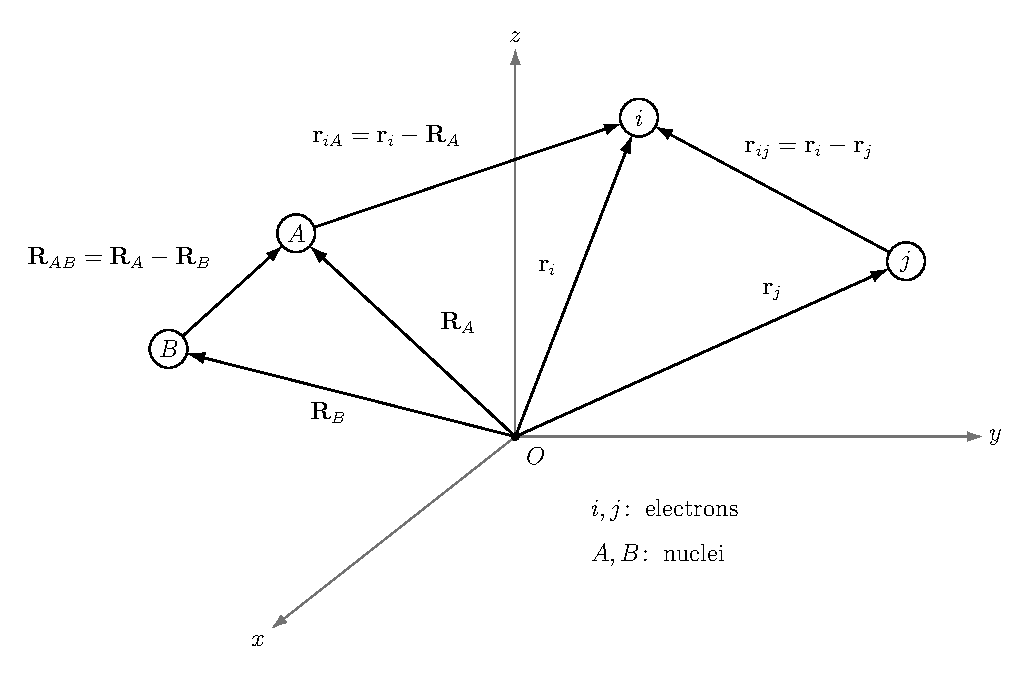
\includegraphics[width=0.62\textwidth]{coord}
  \caption{Electronic and nuclear coordinates entering the molecular
  Hamiltonian.}
  \label{fig:molecular-coordinates}
\end{figure}

In atomic units, for which $m=e=\hbar=1$, these operators read
\begin{subequations}
\begin{align}
  \green{\chT_\text{n}}
  &=
  -\sum_{A=1}^{M}
  \frac{\laplacian_A}{2M_A},
  &
  \blue{\chT_\text{e}}
  &=
  -\sum_{i=1}^{N}
  \frac{\laplacian_i}{2},
  \\
  \orange{\chV_\text{ne}}
  &=
  -\sum_{A=1}^{M}
  \sum_{i=1}^{N}
  \frac{Z_A}{r_{iA}},
  &
  \red{\chV_\text{ee}}
  &=
  \sum_{i<j}^{N}
  \frac{1}{r_{ij}},
  &
  \violet{\chV_\text{nn}}
  &=
  \sum_{A<B}^{M}
  \frac{Z_A Z_B}{R_{AB}}.
\end{align}
\end{subequations}
The quantities $M_A$ and $Z_A$ are the mass and charge of nucleus $A$,
$r_{iA}$ is the distance between electron $i$ and nucleus $A$, $r_{ij}$ is
the distance between electrons $i$ and $j$, and $R_{AB}$ is the distance
between nuclei $A$ and $B$ (see Fig.~\ref{fig:molecular-coordinates}).

Equation~\eqref{eq:total-hamiltonian} defines a formidable quantum
many-body problem. Even if the electron-electron interaction could somehow
be treated exactly, the electronic and nuclear motions would remain coupled.
The key observation behind the Born--Oppenheimer approximation is the large
separation of mass scales between electrons and nuclei. In atomic units, the
electron mass is unity whereas even the lightest nucleus is more than three
orders of magnitude heavier. Correspondingly, the nuclear kinetic-energy
operator contains the small factors $1/M_A$. Nuclear motion is therefore
typically much slower than electronic motion.

This separation of time scales suggests a natural hierarchy. On the
electronic time scale, the nuclei can be regarded as approximately fixed, and
the electrons rapidly adjust to a given nuclear configuration. The first step
is consequently to solve a \red{clamped-nuclei electronic problem}. For fixed
nuclear positions $\{\bR_A\}$, one defines the electronic Hamiltonian
\begin{equation}
  \boxed{
  \chH_\text{elec}
  =
  \blue{\chT_\text{e}}
  +
  \orange{\chV_\text{ne}}
  +
  \red{\chV_\text{ee}}
  }
  \label{eq:electronic-hamiltonian}
\end{equation}
and solves
\begin{equation}
  \chH_\text{elec}
  \Phi_\text{elec}^{(I)}
  (\{\br_i\};\{\bR_A\})
  =
  \cE_\text{elec}^{(I)}(\{\bR_A\})
  \Phi_\text{elec}^{(I)}
  (\{\br_i\};\{\bR_A\}).
  \label{eq:clamped-nuclei}
\end{equation}
The semicolon emphasizes the different roles played by electronic and nuclear
coordinates: the electronic coordinates are genuine variables of
$\Phi_\text{elec}^{(I)}$, whereas the nuclear positions enter
parametrically.

The nuclear repulsion $\chV_\text{nn}$ does not appear in
Eq.~\eqref{eq:electronic-hamiltonian} because, for fixed nuclei, it is simply
a constant with respect to the electronic coordinates. Once the electronic
problem has been solved, it can be added to the electronic energy to define
the energy surface
\begin{equation}
  \boxed{
  U_I(\{\bR_A\})
  =
  \cE_\text{elec}^{(I)}(\{\bR_A\})
  +
  \sum_{A<B}^{M}
  \frac{Z_A Z_B}{R_{AB}}
  }.
  \label{eq:potential-energy-surface}
\end{equation}
Repeating the electronic calculation for different nuclear geometries traces
out a \red{potential-energy surface} (PES). Equilibrium structures correspond
to stationary points of this surface, while chemical reactions, molecular
vibrations, and other nuclear motions can be interpreted in terms of motion
over it.

It is important to distinguish this \emph{clamped-nuclei approximation} from
the Born--Oppenheimer approximation itself. The connection becomes clear by
expanding the exact molecular wavefunction in the complete set of
clamped-nuclei electronic states,
\begin{equation}
  \Phi(\{\br_i\},\{\bR_A\})
  =
  \sum_I
  \Phi_\text{nucl}^{(I)}(\{\bR_A\})
  \Phi_\text{elec}^{(I)}
  (\{\br_i\};\{\bR_A\}).
  \label{eq:born-huang-expansion}
\end{equation}
This Born--Huang expansion is, in principle, exact if the electronic basis is
complete. The electronic and nuclear motions remain coupled because
$\Phi_\text{elec}^{(I)}$ itself changes when the nuclei move. In particular,
the nuclear kinetic-energy operator acts not only on
$\Phi_\text{nucl}^{(I)}$ but also on the parametric dependence of the
electronic wavefunction on $\{\bR_A\}$.

These additional terms generate couplings between different electronic
states. Their leading contributions involve the derivative couplings
\begin{equation}
  \bd_{IJ}^{A}
  =
  \mel{
    \Phi_\text{elec}^{(I)}
  }{
    \nabla_A
  }{
    \Phi_\text{elec}^{(J)}
  },
  \label{eq:nonadiabatic-coupling}
\end{equation}
which measure how rapidly the electronic wavefunctions change as nucleus $A$
moves. The \red{Born--Oppenheimer approximation} consists in neglecting these
nonadiabatic couplings and assuming that nuclear motion takes place on a
single electronic potential-energy surface.

For electronic state $I$, the resulting nuclear Schr\"odinger equation is
\begin{equation}
  \boxed{
  \qty[
    \green{\chT_\text{n}}
    +
    U_I(\{\bR_A\})
  ]
  \Phi_\text{nucl}^{(I)}(\{\bR_A\})
  =
  \cE_\text{tot}
  \Phi_\text{nucl}^{(I)}(\{\bR_A\})
  }.
  \label{eq:nuclear-BO}
\end{equation}
Equivalently,
\begin{equation}
  \boxed{
  \chH_\text{nucl}
  =
  \green{\chT_\text{n}}
  +
  \violet{\chV_\text{nn}}
  +
  \cE_\text{elec}^{(I)}(\{\bR_A\})
  }.
\end{equation}
Thus, within the Born--Oppenheimer picture, the electrons determine the
potential on which the nuclei move.

For a single isolated electronic state, the molecular wavefunction is then
approximated by the product
\begin{equation}
  \boxed{
  \Phi(\{\br_i\},\{\bR_A\})
  \approx
  \Phi_\text{nucl}(\{\bR_A\})
  \Phi_\text{elec}(\{\br_i\};\{\bR_A\})
  }.
  \label{eq:BO-product}
\end{equation}
This familiar factorized form should therefore be viewed as the
\emph{consequence} of neglecting couplings between electronic states rather
than as the starting point of the derivation.

The Born--Oppenheimer approximation is remarkably successful for most
ground-state molecular problems because the electronic wavefunction usually
changes smoothly with the nuclear coordinates and neighboring electronic
states are sufficiently well separated in energy. It becomes less reliable
when two or more electronic states approach one another. Near avoided
crossings, conical intersections, or other regions of strong electronic
near-degeneracy, the derivative couplings in
Eq.~\eqref{eq:nonadiabatic-coupling} can become large and the electronic and
nuclear motions can no longer be treated independently. Such nonadiabatic
effects play a central role, for example, in photochemical processes and
radiationless transitions.

The remainder of this chapter is concerned with the electronic problem.
Unless stated otherwise, the nuclear positions will therefore be regarded as
fixed, and we will seek approximate solutions of the clamped-nuclei
electronic Schr\"odinger equation
\begin{equation}
  \boxed{
  \chH_\text{elec}
  \Phi_\text{elec}
  =
  \cE_\text{elec}
  \Phi_\text{elec}
  }.
  \label{eq:electronic-SE}
\end{equation}
The next question is then not how the nuclei move, but what restrictions must
be imposed on $\Phi_\text{elec}$ because the particles it describes are
indistinguishable fermions. This brings us directly to the Pauli principle
and the antisymmetry of the electronic wavefunction.

\subsubsection{The Pauli principle and antisymmetry}

Having separated the electronic and nuclear motions, we now turn to a second
fundamental ingredient of the electronic problem: electrons are
\red{indistinguishable fermions}. This statement imposes a strict symmetry
requirement on the electronic wavefunction, independently of any
approximation that will later be made to solve the electronic
Schr\"odinger equation.

The non-relativistic electronic Hamiltonian introduced above is spin
independent: it contains the electronic kinetic energy and Coulomb
interactions, but no explicit spin operator. Nevertheless, a complete
description of an electron must contain both its spatial coordinate and its
intrinsic spin degree of freedom. Electrons have spin $s=1/2$, and their spin
functions satisfy
\begin{equation}
  \ket{\omega}=\ket{s,m_s},
  \qquad
  s^2\ket{s,m_s}=s(s+1)\ket{s,m_s},
  \qquad
  s_z\ket{s,m_s}=m_s\ket{s,m_s}.
\end{equation}
The two one-electron spin functions are
\begin{equation}
  \ket{\blue{\alpha}}
  = \ket{\tfrac{1}{2},+\tfrac{1}{2}},
  \qquad
  \ket{\red{\beta}}
  = \ket{\tfrac{1}{2},-\tfrac{1}{2}},
\end{equation}
corresponding respectively to spin-up and spin-down electrons. They form an
orthonormal basis for the one-electron spin space,
\begin{align}
  \int\blue{\alpha}^*(\omega)\red{\beta}(\omega)\dd{\omega}
  &=\int\red{\beta}^*(\omega)\blue{\alpha}(\omega)\dd{\omega}=0,
  &
  \int\blue{\alpha}^*(\omega)\blue{\alpha}(\omega)\dd{\omega}
  &=\int\red{\beta}^*(\omega)\red{\beta}(\omega)\dd{\omega}=1,
  \\
  \braket{\blue{\alpha}}{\red{\beta}}
  &= \braket{\red{\beta}}{\blue{\alpha}}=0,
  &
  \braket{\blue{\alpha}}{\blue{\alpha}}
  &= \braket{\red{\beta}}{\red{\beta}}=1.
\end{align}

It is therefore convenient to combine the spin coordinate $\omega$ and the
spatial coordinate $\br$ into a single composite coordinate,
\begin{equation}
  \boxed{\violet{\bx}=(\orange{\omega},\red{\br})}.
\end{equation}
An $N$-electron wavefunction is consequently a function of $N$ such
coordinates,
\begin{equation}
  \Phi(\bx_1,\bx_2,\ldots,\bx_N).
\end{equation}
Although the Hamiltonian is spin independent in the present treatment, the
spin coordinates are indispensable because the symmetry of the full
spin-spatial wavefunction determines whether the state is compatible with
fermionic statistics.

\paragraph{Indistinguishability and permutation symmetry.}

The labels assigned to identical particles carry no physical information.
Interchanging two electron labels must therefore leave every observable
quantity unchanged. For two particles, this implies in particular that the
probability density satisfies
\begin{equation}
  \abs{\Psi(\red{\bx_1},\blue{\bx_2})}^2
  =
  \abs{\Psi(\blue{\bx_2},\red{\bx_1})}^2.
\end{equation}
The two wavefunctions can thus differ at most by a phase,
\begin{equation}
  \boxed{
  \abs{\Psi(\red{\bx_1},\blue{\bx_2})}^2
  =\abs{\Psi(\blue{\bx_2},\red{\bx_1})}^2
  \quad\Rightarrow\quad
  \Psi(\blue{\bx_2},\red{\bx_1})
  =\green{e^{\ii\theta}}\Psi(\red{\bx_1},\blue{\bx_2}) }.
\end{equation}

Introducing the permutation operator $\chP_{12}$, which exchanges particles
$1$ and $2$, gives
\begin{align}
  \chP_{12}\Psi(\red{\bx_1},\blue{\bx_2})
  &=
  \Psi(\blue{\bx_2},\red{\bx_1})
  =
  \green{e^{\ii\theta}}
  \Psi(\red{\bx_1},\blue{\bx_2}),
  \\
  \chP_{12}^2\Psi(\red{\bx_1},\blue{\bx_2})
  &=
  \green{e^{2\ii\theta}}
  \Psi(\red{\bx_1},\blue{\bx_2})
  =
  \Psi(\red{\bx_1},\blue{\bx_2}).
\end{align}
Because exchanging the same pair twice restores the original labeling,
$\chP_{12}^2=1$, and consequently
\begin{equation}
  \green{e^{2\ii\theta}}=1
  \quad\Rightarrow\quad
  \green{\theta}=n\pi
  \quad\Rightarrow\quad
  \boxed{\green{e^{\ii\theta}}=\pm1}.
\end{equation}

The wavefunction can therefore belong to either a symmetric or an
antisymmetric permutation sector. The plus sign defines \violet{bosons},
for which
\begin{equation}
  \violet{
  \Psi(\bx_1,\bx_2)
  =
  \Psi(\bx_2,\bx_1)
  },
\end{equation}
whereas the minus sign defines \orange{fermions},
\begin{equation}
  \orange{
  \Psi(\bx_1,\bx_2)
  =
  -
  \Psi(\bx_2,\bx_1)
  }.
\end{equation}
Electrons are fermions and must therefore be described by an antisymmetric
wavefunction. The connection between half-integer spin and fermionic
statistics is the content of the spin-statistics theorem; within
non-relativistic quantum mechanics, fermionic antisymmetry is imposed as a
fundamental property of the electronic wavefunction.

For an arbitrary pair of electrons $i$ and $j$, the antisymmetry requirement
can be written compactly as
\begin{equation}
  \boxed{
  \chP_{ij}\Phi=-\Phi
  }.
\end{equation}
The electronic Schr\"odinger equation and Pauli antisymmetry condition are
therefore
\begin{equation}
  \chH_\text{elec}\Phi(\bx_1,\bx_2,\ldots,\bx_N)
  =
  \cE_\text{elec}\Phi(\bx_1,\bx_2,\ldots,\bx_N),
\end{equation}
and
\begin{equation}
  \boxed{
  \Phi(\bx_1,\ldots,\bx_i,\ldots,\bx_j,\ldots,\bx_N)
  =
  -
  \Phi(\bx_1,\ldots,\bx_j,\ldots,\bx_i,\ldots,\bx_N)
  }.
  \label{eq:pauli-antisymmetry}
\end{equation}
Since the electronic Hamiltonian is invariant under the exchange of two
electron labels,
\begin{equation}
  [\chH_\text{elec},\chP_{ij}]=0,
\end{equation}
this antisymmetry is preserved by the electronic dynamics.

\paragraph{The Pauli principle and the exchange hole.}

A particularly important consequence follows immediately from
Eq.~\eqref{eq:pauli-antisymmetry}. If two fermions are assigned the same
composite coordinate, $\bx=\bx_1=\bx_2$, then
\begin{equation}
  \Psi(\bx,\bx)
  =
  -\Psi(\bx,\bx),
\end{equation}
and hence
\begin{equation}
  \boxed{
  \Psi(\bx,\bx)=0
  }.
\end{equation}
The probability of finding two electrons with the same spin at exactly the
same spatial position therefore vanishes. This is one manifestation of the
Pauli exclusion principle.

It is worth emphasizing that the fundamental statement is the
\emph{antisymmetry of the many-electron wavefunction}, not merely the familiar
rule that ``two electrons cannot occupy the same state.'' The latter follows
from the former. If two columns or rows of an antisymmetric fermionic
wavefunction become identical, the wavefunction must vanish.

Antisymmetry also has consequences beyond the special case in which the two
electrons occupy exactly the same point. Conditioning on the presence of one
electron reduces the probability of finding another electron of the same
spin in its vicinity. This deficit in the same-spin pair probability is
called the \red{Fermi hole}, or \red{exchange hole}. It arises entirely from
fermionic antisymmetry and is present even in the absence of dynamical
electron correlation.

We have therefore arrived at a central requirement: any acceptable
many-electron electronic wavefunction must be antisymmetric under the
exchange of two electrons. The next question is how to construct such a
wavefunction from simpler one-electron objects.

\paragraph{Problem.}
\violet{\textit{Given two orthonormal one-electron functions
$\chi_1(\bx)$ and $\chi_2(\bx)$, construct a two-electron fermionic
wavefunction $\Psi(\bx_1,\bx_2)$.}}

\paragraph{Solution.}
Starting from the two possible assignments of the one-electron functions to
the two electrons,
\begin{equation}
  \chi_1(\bx_1)\chi_2(\bx_2)
  \qquad\text{and}\qquad
  \chi_2(\bx_1)\chi_1(\bx_2),
\end{equation}
the required antisymmetric combination is obtained by taking their
difference,
\begin{equation}
  \Psi(\red{\bx_1},\blue{\bx_2})
  =
  \frac{1}{\sqrt{2}}\left[
    \chi_1(\red{\bx_1})\chi_2(\blue{\bx_2})
    -
    \chi_2(\red{\bx_1})\chi_1(\blue{\bx_2})
  \right].
  \label{eq:two-electron-antisym}
\end{equation}
Indeed, exchanging the two electron coordinates immediately yields
\begin{equation}
  \Psi(\bx_2,\bx_1)
  =
  -\Psi(\bx_1,\bx_2).
\end{equation}
For orthonormal $\chi_1$ and $\chi_2$, the prefactor $1/\sqrt{2}$ ensures
normalization.

Slater popularized the determinant representation of this combination,
\begin{equation}
  \boxed{
  \Psi(\red{\bx_1},\blue{\bx_2})
  =
  \frac{1}{\sqrt{2}}
    \begin{vmatrix}
      \chi_1(\red{\bx_1})&\chi_2(\red{\bx_1})\\
      \chi_1(\blue{\bx_2})&\chi_2(\blue{\bx_2})
    \end{vmatrix}
  =
  \frac{1}{\sqrt{2}}\left[
    \chi_1(\red{\bx_1})\chi_2(\blue{\bx_2})
    -
    \chi_2(\red{\bx_1})\chi_1(\blue{\bx_2})
  \right] }.
\end{equation}
The determinant is ideally suited to fermions because interchanging two
electron coordinates corresponds to exchanging two rows of the determinant,
which changes its sign automatically. Likewise, if two one-electron
functions are identical, two columns become identical and the determinant
vanishes. Antisymmetry and the Pauli exclusion principle are therefore built
directly into the determinant structure.

This construction is a \red{Slater determinant}. By contrast, the simple
product
\begin{equation}
  \Psi(\bx_1,\bx_2)
  =
  \chi_1(\bx_1)\chi_2(\bx_2)
\end{equation}
is a \green{Hartree product}. A Hartree product assigns a particular
one-electron function to each labeled electron and is not, by itself,
antisymmetric under particle exchange. It therefore cannot serve as a
fermionic many-electron wavefunction.

The two-electron determinant provides the prototype for the general
$N$-electron construction. Hartree--Fock theory adopts precisely this idea:
the electronic wavefunction is approximated by a single Slater determinant
built from $N$ one-electron spin orbitals. We now turn to this
single-determinant ansatz.

\subsubsection{The single-determinant ansatz}

The previous section established that an acceptable electronic wavefunction
must be antisymmetric with respect to the exchange of any pair of electrons.
A Slater determinant provides the simplest construction that satisfies this
requirement automatically. Hartree--Fock theory takes the decisive additional
step of assuming that the entire $N$-electron wavefunction can be represented
by a \red{single} such determinant.

Thus,
\begin{align}
  \Psi_\text{HF}(\bx_1,\ldots,\bx_N)
  &=
  \frac{1}{\sqrt{N!}}
  \begin{vmatrix}
    \chi_1(\bx_1)&\chi_2(\bx_1)&\cdots&\chi_N(\bx_1)\\
    \chi_1(\bx_2)&\chi_2(\bx_2)&\cdots&\chi_N(\bx_2)\\
    \vdots&\vdots&\ddots&\vdots\\
    \chi_1(\bx_N)&\chi_2(\bx_N)&\cdots&\chi_N(\bx_N)
  \end{vmatrix}
  \nonumber\\
  &\equiv
  \ket{\chi_1(\bx_1)\chi_2(\bx_2)\cdots\chi_N(\bx_N)}
  \nonumber\\
  &=
  \blue{\chA}\left[
    \chi_1(\bx_1)\chi_2(\bx_2)\cdots\chi_N(\bx_N)
  \right]
  =
  \blue{\chA}\green{\Pi(\bx_1,\bx_2,\ldots,\bx_N)}.
  \label{eq:hf-determinant}
\end{align}
Here,
\begin{equation}
  \green{
  \Pi(\bx_1,\bx_2,\ldots,\bx_N)
  =
  \chi_1(\bx_1)\chi_2(\bx_2)\cdots\chi_N(\bx_N)
  }
\end{equation}
is the Hartree product introduced above, while $\blue{\chA}$ is the
antisymmetrizer.

The role of $\chA$ can be made explicit by writing
\begin{equation}
  \boxed{
  \chA
  =
  \frac{1}{\sqrt{N!}}
  \sum_{P}
  (-1)^P \chP
  },
\end{equation}
where the sum runs over the $N!$ permutations of the electron labels,
$\chP$ denotes the corresponding permutation operator, and $(-1)^P$ is
$+1$ for an even permutation and $-1$ for an odd one. Applying $\chA$ to a
Hartree product therefore generates all possible assignments of the
one-electron functions to the electrons with the signs required by
fermionic antisymmetry.

The determinant notation is simply a compact representation of this
antisymmetrized sum. Its usefulness follows directly from elementary
properties of determinants. Exchanging two electron coordinates exchanges
two rows and changes the sign of the determinant. Exchanging two spin
orbitals exchanges two columns and likewise changes its sign. Finally, if
two spin orbitals become identical, two columns coincide and the determinant
vanishes. The Pauli principle is therefore built into the algebraic
structure of the wavefunction.

The normalization factor $1/\sqrt{N!}$ in
Eq.~\eqref{eq:hf-determinant} assumes that the spin orbitals are
orthonormal. Under this condition,
\begin{equation}
  \braket{\Psi_\text{HF}}{\Psi_\text{HF}}=1.
\end{equation}
A normalized Slater determinant is thus completely specified by its $N$
occupied one-electron spin orbitals.

This is a dramatic reduction of the original many-electron problem. Instead
of optimizing an arbitrary function of $N$ electronic coordinates, HF theory
optimizes a set of one-electron functions. The price of this simplification
is that the allowed wavefunctions occupy only a very small subset of the
full antisymmetric $N$-electron Hilbert space. The variational problem is
therefore not to find the exact electronic wavefunction, but to find the
\emph{best single Slater determinant} for the Hamiltonian under
consideration.

\paragraph{Spin orbitals and spatial orbitals.}

Each one-electron function $\chi_p(\bx)$ appearing in the determinant is a
\red{spin orbital}: it depends on both the spatial coordinate $\br$ and the
spin coordinate $\omega$. In the collinear spin formulations considered
initially, a spin orbital separates into spin and spatial factors,
\begin{equation}
  \boxed{
  \chi_p(\bx)
  =
  \red{\sigma(\omega)}
  \blue{\psi_p^\sigma(\br)}
  },
  \qquad
  \sigma(\omega)\in\{\alpha(\omega),\beta(\omega)\}.
  \label{eq:spin-orbital-factorization}
\end{equation}
Thus, a spin orbital is obtained by associating a spatial orbital with either
an $\alpha$ or a $\beta$ spin function.

The distinction between \emph{spin orbital} and \emph{spatial orbital} will
be important throughout the chapter. The Slater determinant itself is built
from spin orbitals because antisymmetry applies to the complete
spin-spatial coordinates of the electrons. In practical molecular
calculations, however, it is usually the spatial functions
$\psi_p^\sigma(\br)$ that are expanded and optimized.

\paragraph{Finite one-electron basis.}

The spatial orbitals are not represented directly as arbitrary continuous
functions. Instead, each is expanded in a finite set of $K$ prescribed basis
functions,
\begin{equation}
  \boxed{
  \blue{\psi_p^\sigma(\br)}
  =
  \sum_{\mu=1}^{K}
  C_{\mu p}^{\sigma}
  \green{\phi_\mu(\br)}
  }.
  \label{eq:lcao-introduction}
\end{equation}
The coefficients $C_{\mu p}^{\sigma}$ then become the quantities to be
determined variationally.

This expansion is conventionally called the \red{linear combination of
atomic orbitals} (LCAO) representation. The terminology is historical:
although the basis functions $\phi_\mu$ are most commonly centered on atoms
in molecular calculations, the essential mathematical point is simply that
the unknown orbitals are represented in a finite one-electron basis.

The finite expansion in Eq.~\eqref{eq:lcao-introduction} introduces a second,
independent approximation on top of the single-determinant ansatz. Even
within Hartree--Fock theory, the exact HF solution is recovered only in the
limit of a complete one-electron basis. The construction, properties, and
convergence of such basis sets will be examined in detail later in this
chapter.

\paragraph{Orthonormality.}

The spin orbitals entering a Slater determinant are chosen to be
orthonormal,
\begin{equation}
\begin{split}
  \braket{\chi_p}{\chi_q}
  &=
  \int
  \chi_p^*(\bx)
  \chi_q(\bx)
  \dd{\bx}
  \\
  &=
  \delta_{pq}
  =
  \begin{cases}
    1,&\text{if $p=q$},\\
    0,&\text{otherwise},
  \end{cases}
\end{split}
\end{equation}
where $\delta_{pq}$ is the Kronecker delta.

This does not imply that the underlying basis functions are themselves
orthogonal. In fact, atom-centered basis functions on different atoms
generally overlap. Their pairwise overlaps define the overlap matrix
\begin{equation}
\begin{split}
  \braket{\phi_\mu}{\phi_\nu}
  &=
  \int
  \phi_\mu^*(\br)
  \phi_\nu(\br)
  \dd{\br}
  \\
  &=S_{\mu\nu}.
\end{split}
\end{equation}
Consequently, the orthonormality of the molecular orbitals imposes a
constraint on the expansion coefficients rather than on the basis functions
themselves. For example, for a given spin sector,
\begin{equation}
  \braket{\psi_p^\sigma}{\psi_q^\sigma}
  =
  \sum_{\mu\nu}
  C_{\mu p}^{\sigma *}
  S_{\mu\nu}
  C_{\nu q}^{\sigma}
  =
  \delta_{pq},
\end{equation}
or, in matrix notation,
\begin{equation}
  \boxed{
  \bC_\sigma^\dagger \bS \bC_\sigma=\bI
  }.
\end{equation}
This distinction between an orthonormal set of molecular orbitals and a
generally nonorthogonal atomic-orbital basis will become central when we
derive the Roothaan--Hall equations.

\paragraph{Restricted and unrestricted Hartree--Fock.}

The single-determinant ansatz still leaves freedom in how the $\alpha$ and
$\beta$ spin orbitals are related. Different constraints on their spatial
parts lead to different variants of Hartree--Fock theory.

In \red{restricted Hartree--Fock} (RHF) theory, appropriate for the usual
closed-shell description, an $\alpha$ electron and a $\beta$ electron in a
pair share the same spatial orbital,
\begin{equation}
  \chi_p^\text{RHF}(\bx)
  =
  \begin{cases}
    \blue{\alpha(\omega)}\psi_p(\br),\\
    \red{\beta(\omega)}\psi_p(\br).
  \end{cases}
  =
  \begin{cases}
    \blue{\psi_p(\br)},\\
    \red{\Bar{\psi}_p(\br)}.
  \end{cases}
\end{equation}
The barred notation will be used when it is convenient to distinguish the
$\beta$ spin orbital associated with a given spatial orbital from its
$\alpha$ partner.

For an even number of electrons in a closed-shell RHF state, each occupied
spatial orbital therefore contains two electrons with opposite spins. Only
$N/2$ distinct occupied spatial orbitals are required to construct the
$N$ occupied spin orbitals.

The restriction that the two spin channels share the same spatial orbitals
can be advantageous: it preserves the closed-shell spin symmetry and reduces
the number of independent orbital coefficients. It is also a genuine
constraint on the variational space. In situations where the optimal
$\alpha$ and $\beta$ electrons would prefer different spatial
distributions, RHF cannot accommodate that relaxation.

The closed-shell RHF ansatz does not describe general open-shell systems. In
\red{unrestricted Hartree--Fock} (UHF) theory, the $\alpha$ and $\beta$
spin components are allowed to use different spatial orbitals,
\begin{equation}
  \chi_p^\text{UHF}(\bx)
  =
  \begin{cases}
    \alpha(\omega)\blue{\psi_p^\alpha(\br)},\\
    \beta(\omega)\red{\psi_p^\beta(\br)}.
  \end{cases}
\end{equation}
This additional variational freedom permits the treatment of open-shell
systems and can also lower the energy of nominally closed-shell systems when
the restricted solution becomes unstable. As we shall see later, however,
this freedom comes at a price: a UHF determinant is generally an eigenfunction
of $\hat S_z$, but not necessarily of $\hat S^2$. The resulting breaking of
spin symmetry is the origin of \red{spin contamination}.

Restricted open-shell Hartree--Fock (ROHF) provides an alternative treatment
of open-shell systems in which the $\alpha$ and $\beta$ electrons retain a
common set of spatial orbitals. We mention this possibility for completeness,
but do not develop the ROHF formalism further here.

\begin{figure}[htbp]
  \centering
  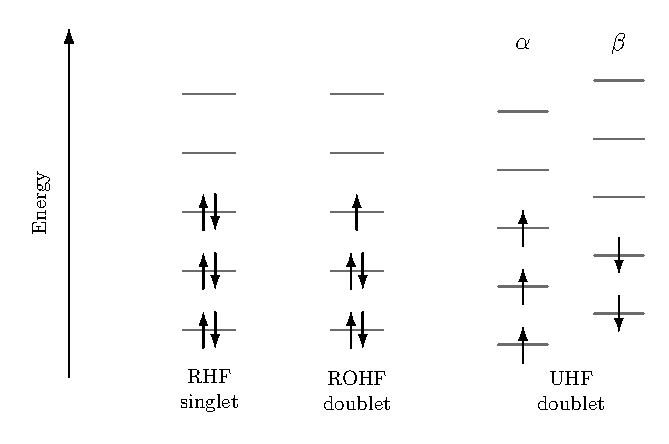
\includegraphics[width=0.72\textwidth]{RHF_UHF}
  \caption{Restricted and unrestricted choices for the spatial parts of the
  spin orbitals. In RHF, paired $\alpha$ and $\beta$ electrons share the same
  spatial orbital, whereas UHF allows the two spin channels to relax
  independently.}
  \label{fig:rhf-uhf-orbitals}
\end{figure}

For RHF, the spatial molecular orbitals form an orthonormal set,
\begin{equation}
  \braket{\psi_p}{\psi_q}
  =
  \int
  \psi_p^*(\br)
  \psi_q(\br)
  \dd{\br}
  =
  \delta_{pq}.
\end{equation}
For UHF, orthonormality holds separately within each spin sector,
\begin{align}
  \braket{\psi_p^\alpha}{\psi_q^\alpha}
  &=
  \int
  \psi_p^{\alpha*}(\br)
  \psi_q^\alpha(\br)
  \dd{\br}
  =
  \delta_{pq},
  \\
  \braket{\psi_p^\beta}{\psi_q^\beta}
  &=
  \int
  \psi_p^{\beta*}(\br)
  \psi_q^\beta(\br)
  \dd{\br}
  =
  \delta_{pq},
\end{align}
whereas opposite-spin spatial orbitals need not be orthogonal,
\begin{equation}
  \braket{\psi_p^\alpha}{\psi_q^\beta}
  =
  \int
  \psi_p^{\alpha*}(\br)
  \psi_q^\beta(\br)
  \dd{\br}
  =
  S_{pq}^{\alpha\beta}.
\end{equation}
There is no contradiction with the orthonormality of the full spin orbitals:
because
\begin{equation}
  \braket{\alpha}{\beta}=0,
\end{equation}
an $\alpha$ spin orbital and a $\beta$ spin orbital are orthogonal regardless
of the overlap between their spatial parts.

This distinction is useful to keep in mind. In UHF, one may have
\begin{equation}
  \braket{\psi_p^\alpha}{\psi_q^\beta}\neq0,
  \qquad\text{but}\qquad
  \braket{
    \alpha\psi_p^\alpha
  }{
    \beta\psi_q^\beta
  }=0.
\end{equation}

\paragraph{Orbital spaces and index conventions.}

We conclude by fixing the notation used throughout the remainder of the
chapter. The one-electron spaces are
\begin{align}
  \{\phi_\mu\mid\mu=1,\ldots,K\}
  &:\quad
  \green{\text{basis functions or atomic orbitals (AOs)}},
  \\
  \{\psi_p\mid p=1,\ldots,K\}
  &:\quad
  \violet{\text{restricted spatial orbitals or molecular orbitals (MOs)}},
  \\
  \{\chi_p\mid p=1,\ldots,2K\}
  &:\quad
  \orange{\text{spin orbitals}}.
\end{align}
Thus, a basis of $K$ spatial functions generates $K$ spatial molecular
orbitals and, when the two spin functions are included, $2K$ spin orbitals.

Unless otherwise stated, the following index convention will be used:
\begin{equation}
  \boxed{
  \begin{array}{ccl}
    \mu,\nu,\lambda,\sigma,\ldots
      &:& \text{basis functions / AOs},
    \\[1mm]
    p,q,r,s,\ldots
      &:& \text{general orbitals},
    \\[1mm]
    i,j,k,l,\ldots
      &:& \text{occupied orbitals},
    \\[1mm]
    a,b,c,d,\ldots
      &:& \text{unoccupied or virtual orbitals}.
  \end{array}
  }
\end{equation}
Among the $2K$ spin orbitals, $N$ are occupied in the HF determinant and are
therefore labeled by $i,j,k,l,\ldots$. The remaining $2K-N$ spin orbitals are
unoccupied. They are variously called \red{vacant}, \red{unoccupied}, or
\red{virtual} orbitals and are labeled by $a,b,c,d,\ldots$.

The distinction between occupied and virtual orbitals is relative to the
particular determinant under consideration. Only the occupied orbitals enter
the Slater determinant explicitly, but the virtual orbitals provide the
complementary one-electron space and will become essential when discussing
orbital optimization, excited determinants, response, and correlated
electronic-structure methods.

Finally, a system with \red{two electrons in each occupied spatial orbital}
is called \red{closed shell}. Otherwise, it is \red{open shell}. For the
ground state of a closed-shell system containing an even number $N$ of
electrons, the first $N/2$ spatial orbitals are doubly occupied,
\begin{equation}
  \psi_1^2\psi_2^2\cdots\psi_{N/2}^2,
\end{equation}
while the remaining $K-N/2$ spatial orbitals are vacant.

The single-determinant ansatz, together with these orthonormality constraints,
defines the variational space of Hartree--Fock theory. The next step is to
determine which determinant within this space is optimal. This requires
evaluating the expectation value of the electronic Hamiltonian as a functional
of the occupied orbitals.

\subsection{The Hartree--Fock energy functional}
\subsubsection{Energy expectation value}

We have now specified the class of wavefunctions allowed within
Hartree--Fock theory: normalized single Slater determinants constructed from
orthonormal spin orbitals. The remaining question is variational. Among all
such determinants, which one provides the lowest possible energy?

For fixed nuclear positions, the electronic energy associated with a given
Slater determinant is the expectation value of the electronic Hamiltonian,
\begin{equation}
  \boxed{
  \EHF
  =
  \mel{\Psi_\text{HF}}{\chH_\text{elec}}{\Psi_\text{HF}}
  },
  \qquad
  \chH_\text{elec}
  =
  \blue{\chT_\text{e}}
  +
  \orange{\chV_\text{ne}}
  +
  \red{\chV_\text{ee}}.
  \label{eq:hf-expectation-value}
\end{equation}
Since $\Psi_\text{HF}$ depends on the occupied spin orbitals, this expression
should be regarded as an \red{energy functional},
\begin{equation}
  \EHF
  =
  \EHF[\chi_1,\chi_2,\ldots,\chi_N].
\end{equation}
Hartree--Fock theory seeks the stationary point---and, for the ground-state
solution, the minimum---of this functional subject to the orthonormality
constraints
\begin{equation}
  \braket{\chi_i}{\chi_j}=\delta_{ij}.
\end{equation}

The variational principle guarantees that the energy of any normalized trial
wavefunction lies above or at the exact ground-state energy,
\begin{equation}
  \mel{\Psi_\text{trial}}{\chH_\text{elec}}{\Psi_\text{trial}}
  \geq
  \cE_\text{elec}^{(0)}.
\end{equation}
Hartree--Fock therefore finds the lowest energy accessible within the
restricted manifold of single determinants. The remaining difference between
this optimal single-determinant energy and the exact non-relativistic
electronic energy is associated with electron correlation beyond the HF
description.

\paragraph{One- and two-electron operators.}

It is useful to separate the electronic Hamiltonian into one- and
two-electron parts,
\begin{equation}
  \boxed{
  \chH_\text{elec}
  =
  \chO_1+\chO_2
  =
  \sum_{i=1}^{N}\hh(\bx_i)
  +
  \sum_{i<j}^{N}\frac{1}{r_{ij}}
  }.
  \label{eq:one-two-electron-hamiltonian}
\end{equation}
The one-electron, or \red{core}, Hamiltonian is
\begin{equation}
  \boxed{
  \hh(\bx_i)
  =
  -\frac{\laplacian_i}{2}
  -
  \sum_{A=1}^{M}\frac{Z_A}{r_{iA}}
  },
\end{equation}
so that
\begin{equation}
  \chO_1
  =
  \sum_{i=1}^{N}\hh(\bx_i).
\end{equation}
It contains the kinetic energy of electron $i$ and its attraction to all
nuclei. The explicit electron-electron interaction is contained in the
two-electron operator
\begin{equation}
  \boxed{
  \chO_2
  =
  \red{\chV_\text{ee}}
  =
  \sum_{i<j}^{N}\frac{1}{r_{ij}}
  }.
\end{equation}

The distinction between one- and two-electron operators is important because
their expectation values over a Slater determinant have particularly simple
forms. This simplification is one of the main reasons why the
single-determinant ansatz is computationally tractable.

\paragraph{One-electron contribution.}

For a normalized determinant constructed from orthonormal spin orbitals, the
Slater--Condon rules reduce the expectation value of a one-electron operator
to a sum over the occupied spin orbitals,
\begin{equation}
  \mel{\Psi_\text{HF}}{\chO_1}{\Psi_\text{HF}}
  =
  \sum_{i=1}^{N}
  \mel{\chi_i}{\hh}{\chi_i}.
\end{equation}
Introducing
\begin{equation}
  h_{ij}
  =
  \mel{\chi_i}{\hh}{\chi_j},
\end{equation}
we obtain simply
\begin{equation}
  \boxed{
  \mel{\Psi_\text{HF}}{\chO_1}{\Psi_\text{HF}}
  =
  \sum_{i=1}^{N}h_{ii}
  }.
  \label{eq:hf-one-electron-energy}
\end{equation}
Thus, the one-electron part of the HF energy is obtained by adding the kinetic
and electron-nuclear energies associated with each occupied spin orbital.

The nucleus-nucleus repulsion does not belong to the electronic Hamiltonian
because, within the clamped-nuclei problem, it contains no electronic
coordinates. Nevertheless, it must be added when the total
Born--Oppenheimer energy is required. For a normalized electronic
wavefunction,
\begin{equation}
  \mel{\Psi_\text{HF}}{\violet{\chV_\text{nn}}}{\Psi_\text{HF}}
  =
  \violet{V_\text{nn}}
  \braket{\Psi_\text{HF}}{\Psi_\text{HF}}
  =
  \violet{V_\text{nn}}
  \qquad\text{if}\qquad
  \braket{\Psi_\text{HF}}{\Psi_\text{HF}}=1.
\end{equation}
Hence,
\begin{equation}
  \boxed{
  E_\text{tot}^\text{HF}
  =
  \EHF+V_\text{nn}
  }.
\end{equation}
In what follows, $\EHF$ will denote the electronic Hartree--Fock energy
unless stated otherwise.

\paragraph{Two-electron contribution: Coulomb and exchange.}

The effect of antisymmetry first appears explicitly in the expectation value
of the electron-electron interaction. For each pair of occupied spin
orbitals, two contributions arise,
\begin{align}
  \mel{\Psi_\text{HF}}{\chO_2}{\Psi_\text{HF}}
  &=
  \sum_{i<j}^{N}
  \left[
    \mel{\chi_i(\bx_1)\chi_j(\bx_2)}{r_{12}^{-1}}
        {\chi_i(\bx_1)\chi_j(\bx_2)}
  \right.
  \nonumber\\
  &\hspace{7em}\left.
    -
    \mel{\chi_i(\bx_1)\chi_j(\bx_2)}{r_{12}^{-1}}
        {\chi_j(\bx_1)\chi_i(\bx_2)}
  \right]
  \nonumber\\
  &=
  \sum_{i<j}^{N}
  \left(
    \underbrace{\cJ_{ij}}_{\green{\text{Coulomb}}}
    -
    \underbrace{\cK_{ij}}_{\red{\text{exchange}}}
  \right).
  \label{eq:hf-two-electron-energy}
\end{align}

The first term,
\begin{equation}
  \boxed{
  \cJ_{ij}
  =
  \mel{\chi_i(\bx_1)\chi_j(\bx_2)}{r_{12}^{-1}}
       {\chi_i(\bx_1)\chi_j(\bx_2)}
  },
\end{equation}
is the \green{Coulomb integral}. Written explicitly,
\begin{equation}
  \cJ_{ij}
  =
  \iint
  \chi_i^*(\bx_1)\chi_j^*(\bx_2)
  \frac{1}{r_{12}}
  \chi_i(\bx_1)\chi_j(\bx_2)
  \dd{\bx_1}\dd{\bx_2}.
  \label{eq:coulomb-integral}
\end{equation}
It has a direct classical interpretation: it is the electrostatic repulsion
between the charge distributions associated with orbitals $i$ and $j$.

The second term,
\begin{equation}
  \boxed{
  \cK_{ij}
  =
  \mel{\chi_i(\bx_1)\chi_j(\bx_2)}{r_{12}^{-1}}
       {\chi_j(\bx_1)\chi_i(\bx_2)}
  },
\end{equation}
is the \red{exchange integral},
\begin{equation}
  \cK_{ij}
  =
  \iint
  \chi_i^*(\bx_1)\chi_j^*(\bx_2)
  \frac{1}{r_{12}}
  \chi_j(\bx_1)\chi_i(\bx_2)
  \dd{\bx_1}\dd{\bx_2}.
  \label{eq:exchange-integral}
\end{equation}
Unlike $\cJ_{ij}$, the exchange contribution has no classical electrostatic
counterpart. It arises entirely from the antisymmetry of the fermionic
wavefunction: it is the energetic signature of the exchange of electron
labels between the two terms of the determinant.

This point is fundamental. The Coulomb interaction itself is the same
$1/r_{12}$ operator as before; there is no separate ``exchange force'' in the
Hamiltonian. Exchange appears because the expectation value of the Coulomb
operator is evaluated with an antisymmetric wavefunction.

Because the spin orbitals factorize into spin and spatial parts, the exchange
integral also carries an important spin selection rule. If $\chi_i$ and
$\chi_j$ have opposite spin,
\begin{equation}
  \braket{\alpha}{\beta}=0
  \qquad\Longrightarrow\qquad
  \boxed{\cK_{ij}=0}.
\end{equation}
Exchange therefore acts only between electrons of the same spin in the
collinear RHF and UHF formulations considered here. Coulomb interactions, by
contrast, are present between every pair of electrons regardless of spin.

\paragraph{Self-interaction cancellation.}

The pairwise form of the two-electron energy can equivalently be written as a
double sum,
\begin{equation}
  \mel{\Psi_\text{HF}}{\chO_2}{\Psi_\text{HF}}
  =
  \frac{1}{2}
  \sum_{i=1}^{N}
  \sum_{j=1}^{N}
  \left(
    \cJ_{ij}-\cK_{ij}
  \right).
  \label{eq:hf-double-sum}
\end{equation}
The factor $1/2$ avoids counting every distinct electron pair twice.

At first sight, the terms with $i=j$ in this expression might appear to
describe the Coulomb interaction of an electron with itself. However,
\begin{equation}
  \red{
  \boxed{
  \cJ_{ii}=\cK_{ii}
  }
  },
\end{equation}
because
\begin{equation}
  \cJ_{ii}
  =
  \cK_{ii}
  =
  \iint
  \frac{
  \abs{\chi_i(\bx_1)}^2
  \abs{\chi_i(\bx_2)}^2
  }{r_{12}}
  \dd{\bx_1}\dd{\bx_2}.
\end{equation}
Consequently,
\begin{equation}
  \cJ_{ii}-\cK_{ii}=0.
\end{equation}
The spurious Coulomb self-interaction is therefore cancelled exactly by
exchange in Hartree--Fock theory.

Combining the one- and two-electron contributions gives the fundamental HF
energy expression
\begin{equation}
  \boxed{
  \EHF
  =
  \sum_{i=1}^{N}h_{ii}
  +
  \sum_{i<j}^{N}
  \left(
    \cJ_{ij}-\cK_{ij}
  \right)
  }.
  \label{eq:hf-energy-spin-orbitals}
\end{equation}
Equivalently,
\begin{equation}
  \boxed{
  \EHF
  =
  \sum_{i=1}^{N}h_{ii}
  +
  \frac{1}{2}
  \sum_{i=1}^{N}
  \sum_{j=1}^{N}
  \left(
    \cJ_{ij}-\cK_{ij}
  \right)
  }.
  \label{eq:hf-energy-spin-orbitals-double}
\end{equation}

This expression already reveals the central structure of HF theory. The
energy depends on each occupied orbital individually through $h_{ii}$, but
also on every pair of occupied orbitals through the Coulomb and exchange
terms. The orbitals therefore cannot be optimized independently: changing
one orbital changes the effective field experienced by all the others. This
coupling is the origin of the self-consistent character of the Hartree--Fock
equations.

\paragraph{Coulomb operator.}

It is useful to promote the Coulomb and exchange integrals to one-electron
operators. For a fixed occupied spin orbital $\chi_j$, the Coulomb operator
$\chJ_j$ acts on $\chi_i$ as
\begin{equation}
  \chJ_j(\bx_1)\ket{\chi_i(\bx_1)}
  =
  \mel{\chi_j(\bx_2)}{r_{12}^{-1}}{\chi_j(\bx_2)}
  \ket{\chi_i(\bx_1)},
\end{equation}
or explicitly,
\begin{equation}
  \boxed{
  \chJ_j(\bx_1)\ket{\chi_i(\bx_1)}
  =
  \left[
    \int
    \chi_j^*(\bx_2)
    \frac{1}{r_{12}}
    \chi_j(\bx_2)
    \dd{\bx_2}
  \right]
  \ket{\chi_i(\bx_1)}
  }.
  \label{eq:coulomb-operator}
\end{equation}
The quantity in square brackets is the electrostatic potential generated by
the density of orbital $j$ at the position of electron $1$.

Its expectation value is
\begin{align}
  \cJ_{ij}
  &=
  \mel{\chi_i(\bx_1)}
       {\chJ_j(\bx_1)}
       {\chi_i(\bx_1)}
  \nonumber\\
  &=
  \mel{\chi_i(\bx_1)\chi_j(\bx_2)}
       {r_{12}^{-1}}
       {\chi_i(\bx_1)\chi_j(\bx_2)}
  \nonumber\\
  &=
  \iint
  \chi_i^*(\bx_1)
  \chi_j^*(\bx_2)
  \frac{1}{r_{12}}
  \chi_i(\bx_1)
  \chi_j(\bx_2)
  \dd{\bx_1}\dd{\bx_2}.
\end{align}

The Coulomb operator is \red{local} in the usual one-particle sense. Once the
integration over $\bx_2$ has been carried out, it acts on $\chi_i(\bx_1)$ by
multiplication with a function of $\bx_1$,
\begin{equation}
  \chJ_j(\bx_1)\chi_i(\bx_1)
  =
  J_j(\bx_1)\chi_i(\bx_1).
\end{equation}
Every orbital acted upon by $\chJ_j$ therefore experiences the same
multiplicative Coulomb potential generated by orbital $j$.

\paragraph{Exchange operator.}

The exchange operator has a qualitatively different structure. Its action is
defined by
\begin{equation}
  \chK_j(\bx_1)\ket{\chi_i(\bx_1)}
  =
  \mel{\chi_j(\bx_2)}{r_{12}^{-1}}{\chi_i(\bx_2)}
  \ket{\chi_j(\bx_1)},
\end{equation}
or explicitly,
\begin{equation}
  \boxed{
  \chK_j(\bx_1)\ket{\chi_i(\bx_1)}
  =
  \left[
    \int
    \chi_j^*(\bx_2)
    \frac{1}{r_{12}}
    \chi_i(\bx_2)
    \dd{\bx_2}
  \right]
  \ket{\chi_j(\bx_1)}
  }.
  \label{eq:exchange-operator}
\end{equation}
Its matrix element is
\begin{align}
  \cK_{ij}
  &=
  \mel{\chi_i(\bx_1)}
       {\chK_j(\bx_1)}
       {\chi_i(\bx_1)}
  \nonumber\\
  &=
  \mel{\chi_i(\bx_1)\chi_j(\bx_2)}
       {r_{12}^{-1}}
       {\chi_j(\bx_1)\chi_i(\bx_2)}
  \nonumber\\
  &=
  \iint
  \chi_i^*(\bx_1)
  \chi_j^*(\bx_2)
  \frac{1}{r_{12}}
  \chi_j(\bx_1)
  \chi_i(\bx_2)
  \dd{\bx_1}\dd{\bx_2}.
\end{align}

Unlike the Coulomb operator, $\chK_j$ is \red{nonlocal}. Its value at
$\bx_1$ depends on the values of the orbital on which it acts,
$\chi_i(\bx_2)$, over all coordinates $\bx_2$. Moreover, the resulting
function is proportional to $\chi_j(\bx_1)$ rather than simply to
$\chi_i(\bx_1)$. Exchange therefore cannot, in general, be represented by a
single multiplicative potential.

This distinction between the local Coulomb operator and the nonlocal exchange
operator is one of the defining features of Hartree--Fock theory. Both arise
from the same electron-electron Coulomb interaction, but the exchange term
is generated solely by the antisymmetry of the Slater determinant.

The HF energy can therefore be regarded as a functional of the occupied
orbitals,
\begin{equation}
  \boxed{
  \EHF[\{\chi_i\}]
  =
  \sum_i
  \mel{\chi_i}{\hh}{\chi_i}
  +
  \frac{1}{2}
  \sum_{ij}
  \left(
    \cJ_{ij}-\cK_{ij}
  \right)
  },
  \qquad
  \braket{\chi_i}{\chi_j}=\delta_{ij}.
  \label{eq:hf-energy-functional}
\end{equation}
The remainder of Hartree--Fock theory consists essentially in minimizing this
functional with respect to the occupied orbitals while preserving their
orthonormality. Before carrying out that minimization, however, it is useful
to introduce a compact notation for the one- and two-electron integrals
appearing throughout the theory.

\subsubsection{One- and two-electron integrals}

The Hartree--Fock energy derived in the previous section is expressed entirely
in terms of matrix elements of one- and two-electron operators. These
quantities occur throughout electronic-structure theory, so it is useful to
introduce their notation carefully at this stage.

There are two widely used conventions for two-electron integrals:
\red{physicists' notation} and \red{chemists' notation}. They describe
exactly the same mathematical objects, but group the four orbital indices
differently. Confusion between these conventions is a frequent source of
index errors, particularly when moving between quantum-chemistry and
many-body-theory literature.

\paragraph{One-electron integrals.}

For a general one-electron operator $\hh$, the matrix element between spin
orbitals $\chi_i$ and $\chi_j$ is
\begin{equation}
  \boxed{
  \mel{i}{\hh}{j}
  =
  h_{ij}
  =
  \mel{\chi_i}{\hh}{\chi_j}
  =
  \int
  \chi_i^*(\bx_1)
  \hh(\bx_1)
  \chi_j(\bx_1)
  \dd{\bx_1}
  }.
  \label{eq:one-electron-integral}
\end{equation}
For the Hartree--Fock problem, $\hh$ is the core Hamiltonian,
\begin{equation}
  \hh(\bx)
  =
  -\frac{\laplacian}{2}
  -
  \sum_A\frac{Z_A}{r_A},
\end{equation}
so that $h_{ij}$ contains both the electronic kinetic energy and the
electron-nuclear attraction.

Since $\hh$ is Hermitian,
\begin{equation}
  \boxed{
  h_{ij}=h_{ji}^*
  }.
\end{equation}
For real orbitals and a real one-electron operator, this reduces to
\begin{equation}
  h_{ij}=h_{ji}.
\end{equation}

In Mulliken notation, the same one-electron integral may equivalently be
written
\begin{equation}
  \rmel{i}{\hh}{j}
  =
  h_{ij}
  =
  \rmel{\chi_i}{\hh}{\chi_j}
  =
  \int
  \chi_i^*(\bx_1)
  \hh(\bx_1)
  \chi_j(\bx_1)
  \dd{\bx_1}.
\end{equation}
Thus, for one-electron quantities, the distinction between physicists' and
chemists' notation is essentially cosmetic. The important difference appears
for two-electron integrals.

\paragraph{Electron-repulsion integrals: physicists' notation.}

The matrix element of the Coulomb interaction between two-electron product
states defines an \red{electron-repulsion integral} (ERI). In physicists'
notation,
\begin{equation}
  \boxed{
  \braket{ij}{kl}
  =
  \braket{\chi_i\chi_j}{\chi_k\chi_l}
  =
  \iint
  \chi_i^*(\bx_1)
  \chi_j^*(\bx_2)
  \frac{1}{r_{12}}
  \chi_k(\bx_1)
  \chi_l(\bx_2)
  \dd{\bx_1}\dd{\bx_2}
  }.
  \label{eq:eri-physicists}
\end{equation}
The ordering of the indices reflects the underlying braket structure:
$i$ and $j$ label the two orbitals in the bra, whereas $k$ and $l$ label
those in the ket. More importantly, the first and third indices refer to
electron coordinate $\bx_1$, while the second and fourth refer to $\bx_2$:
\begin{equation}
  \braket{
    \underbrace{i}_{\bx_1}
    \underbrace{j}_{\bx_2}
  }{
    \underbrace{k}_{\bx_1}
    \underbrace{l}_{\bx_2}
  }.
\end{equation}

With this notation, the Coulomb and exchange integrals introduced in the
previous section are simply
\begin{equation}
  \boxed{
  \cJ_{ij}=\braket{ij}{ij},
  \qquad
  \cK_{ij}=\braket{ij}{ji}
  }.
  \label{eq:JK-physicists}
\end{equation}
The only difference between the two is therefore the permutation of the two
indices in the ket.

This observation motivates the introduction of the
\red{antisymmetrized two-electron integral},
\begin{equation}
  \boxed{
  \mel{ij}{}{kl}
  =
  \braket{ij}{kl}
  -
  \braket{ij}{lk}
  }.
  \label{eq:antisymmetrized-eri}
\end{equation}
Explicitly,
\begin{align}
  \mel{ij}{}{kl}
  &=
  \iint
  \chi_i^*(\bx_1)
  \chi_j^*(\bx_2)
  \frac{1}{r_{12}}
  \left[
    \chi_k(\bx_1)\chi_l(\bx_2)
    -
    \chi_l(\bx_1)\chi_k(\bx_2)
  \right]
  \dd{\bx_1}\dd{\bx_2}
  \nonumber\\
  &=
  \iint
  \chi_i^*(\bx_1)
  \chi_j^*(\bx_2)
  \frac{1}{r_{12}}
  (1-\chP_{12})
  \chi_k(\bx_1)\chi_l(\bx_2)
  \dd{\bx_1}\dd{\bx_2}.
\end{align}
The antisymmetrized integral combines the direct Coulomb contribution and
its exchange counterpart into a single object. For example,
\begin{equation}
  \boxed{
  \mel{ij}{}{ij}
  =
  \cJ_{ij}-\cK_{ij}
  }.
\end{equation}
The HF energy can therefore also be written compactly as
\begin{equation}
  \EHF
  =
  \sum_i h_{ii}
  +
  \frac{1}{2}
  \sum_{ij}
  \mel{ij}{}{ij}.
\end{equation}

As expected from its definition, the antisymmetrized integral changes sign
upon exchanging either pair of fermionic indices,
\begin{equation}
  \mel{ij}{}{kl}
  =
  -\mel{ji}{}{kl}
  =
  -\mel{ij}{}{lk}
  =
  \mel{ji}{}{lk}.
\end{equation}
This notation becomes particularly convenient in post-Hartree--Fock and
many-body perturbation theories, where direct and exchange contributions
repeatedly occur together.

\paragraph{Mulliken or chemists' notation.}

Quantum-chemistry literature very often uses a different grouping of the
same four orbital indices. In Mulliken, or chemists', notation,
\begin{equation}
  \boxed{
  \rbraket{ij}{kl}
  =
  \rbraket{\chi_i\chi_j}{\chi_k\chi_l}
  =
  \iint
  \chi_i^*(\bx_1)
  \chi_j(\bx_1)
  \frac{1}{r_{12}}
  \chi_k^*(\bx_2)
  \chi_l(\bx_2)
  \dd{\bx_1}\dd{\bx_2}
  }.
  \label{eq:eri-chemists}
\end{equation}
Here, the first pair of indices belongs to electron coordinate $\bx_1$ and
the second pair belongs to electron coordinate $\bx_2$:
\begin{equation}
  \rbraket{
    \underbrace{ij}_{\bx_1}
  }{
    \underbrace{kl}_{\bx_2}
  }.
\end{equation}

The two notations therefore differ only by an index permutation. Comparing
Eqs.~\eqref{eq:eri-physicists} and \eqref{eq:eri-chemists} gives
\begin{equation}
  \boxed{
  \braket{ij}{kl}
  =
  \rbraket{ik}{jl}
  }.
  \label{eq:phys-chem-map}
\end{equation}
This simple correspondence is worth remembering:
\begin{equation}
  \boxed{
  \text{physicists: }\braket{ij}{kl}
  \qquad\longleftrightarrow\qquad
  \text{chemists: }\rbraket{ik}{jl}
  }.
\end{equation}

Consequently, the Coulomb and exchange integrals become
\begin{equation}
  \boxed{
  \cJ_{ij}
  =
  \rbraket{ii}{jj},
  \qquad
  \cK_{ij}
  =
  \rbraket{ij}{ji}
  }
  \qquad
  \text{(chemists' notation)}.
\end{equation}
These expressions also make the physical interpretation transparent:
$\cJ_{ij}$ couples the densities $\chi_i^*\chi_i$ and
$\chi_j^*\chi_j$, whereas $\cK_{ij}$ couples the transition-like products
$\chi_i^*\chi_j$ and $\chi_j^*\chi_i$.

The same notation will be used throughout this chapter for integrals over
spin orbitals and over spatial orbitals; the surrounding context specifies
which type is intended.

\paragraph{Spin selection rules.}

When the $\chi_p$ are collinear spin orbitals,
\begin{equation}
  \chi_p(\bx)
  =
  \sigma_p(\omega)\psi_p(\br),
\end{equation}
integration over the spin coordinates gives
\begin{equation}
  \braket{ij}{kl}
  =
  \delta_{\sigma_i\sigma_k}
  \delta_{\sigma_j\sigma_l}
  \iint
  \psi_i^*(\br_1)
  \psi_j^*(\br_2)
  \frac{1}{r_{12}}
  \psi_k(\br_1)
  \psi_l(\br_2)
  \dd{\br_1}\dd{\br_2}.
\end{equation}
A spin-orbital ERI therefore vanishes unless the spin on each electron line
is conserved,
\begin{equation}
  \sigma_i=\sigma_k,
  \qquad
  \sigma_j=\sigma_l.
\end{equation}
For the exchange integral,
\begin{equation}
  \cK_{ij}=\braket{ij}{ji},
\end{equation}
this requires $\sigma_i=\sigma_j$. Hence,
\begin{equation}
  \boxed{
  \cK_{ij}=0
  \qquad
  \text{for opposite-spin orbitals}
  }.
\end{equation}
This is the integral form of the same-spin nature of Hartree--Fock exchange
discussed in the previous section.

\paragraph{Permutation symmetries.}

Electron-repulsion integrals possess extensive permutation symmetries. These
follow from three simple properties: the symmetry of the Coulomb operator
under interchange of the two electrons, its Hermiticity, and, for real
orbitals, the commutativity of the orbital products evaluated at a common
coordinate.

For reference, the physicists' ERI is
\begin{equation}
  \braket{ij}{kl}
  =
  \braket{\chi_i\chi_j}{\chi_k\chi_l}
  =
  \iint
  \chi_i^*(\bx_1)
  \chi_j^*(\bx_2)
  \frac{1}{r_{12}}
  \chi_k(\bx_1)
  \chi_l(\bx_2)
  \dd{\bx_1}\dd{\bx_2}.
\end{equation}
For \red{complex-valued integrals}, physicists' ERIs obey
\begin{equation}
  \boxed{
  \braket{ij}{kl}
  =
  \braket{ji}{lk}
  =
  \braket{kl}{ij}^*
  =
  \braket{lk}{ji}^*
  }.
  \label{eq:eri-complex-symmetry}
\end{equation}
The first equality corresponds to exchanging the two electron coordinates,
while the complex-conjugated relations follow from Hermiticity.

For \green{real-valued integrals}, this becomes
\begin{align}
  \braket{ij}{kl}
  &=
  \braket{ji}{lk}
  =
  \braket{kl}{ij}
  =
  \braket{lk}{ji}
  \nonumber\\
  &=
  \braket{kj}{il}
  =
  \braket{jk}{li}
  =
  \braket{il}{kj}
  =
  \braket{li}{jk}
  \label{eq:eri-physicists-eightfold}
\end{align}

In chemists' notation, the defining integral is
\begin{equation}
  \rbraket{ij}{kl}
  =
  \rbraket{\chi_i\chi_j}{\chi_k\chi_l}
  =
  \iint
  \chi_i^*(\bx_1)
  \chi_j(\bx_1)
  \frac{1}{r_{12}}
  \chi_k^*(\bx_2)
  \chi_l(\bx_2)
  \dd{\bx_1}\dd{\bx_2}.
\end{equation}
For \green{real-valued integrals}, its symmetry relations take the familiar
form
\begin{align}
  \rbraket{ij}{kl}
  &=
  \rbraket{ji}{kl}
  =
  \rbraket{ij}{lk}
  =
  \rbraket{ji}{lk}
  \nonumber\\
  &=
  \rbraket{kl}{ij}
  =
  \rbraket{lk}{ij}
  =
  \rbraket{kl}{ji}
  =
  \rbraket{lk}{ji}
  \label{eq:eri-chemists-eightfold}
\end{align}
Thus, for real-valued orbitals, ERIs possess
\red{eightfold permutation symmetry}.

This symmetry has an important computational consequence. A naive set of
$K$ one-electron basis functions generates $K^4$ four-index ERIs,
\begin{equation}
  \rbraket{\mu\nu}{\lambda\sigma}.
\end{equation}
However, many of these entries are identical by permutation symmetry.
For four distinct indices, up to eight nominally different integrals
represent the same numerical quantity. Modern integral algorithms exploit
these symmetries extensively to reduce both the amount of computation and
the storage required for the two-electron integrals.

The apparent $K^4$ growth nevertheless makes the treatment of ERIs one of
the central computational challenges of conventional electronic-structure
theory. Later in this chapter, when the basis functions themselves are
introduced in detail, we will return to the evaluation of these integrals
and to the algorithms that make their computation practical.

\subsubsection{Worked examples}

The general expressions derived above can appear rather compact when first
encountered. It is therefore useful to recover them explicitly for systems
containing only a few electrons. These examples illustrate how the
orthonormality of the spin orbitals and the antisymmetry of the Slater
determinant combine to produce the characteristic Hartree--Fock energy
expression.

We begin with two electrons occupying the orthonormal spin orbitals
$\chi_1$ and $\chi_2$. Throughout the following examples, the shorthand
\begin{equation}
  \chi_p(i)\equiv\chi_p(\bx_i)
\end{equation}
will be used, where $i$ labels the complete spin-spatial coordinate of
electron $i$.

% ============================================================================
% Normalization
% ============================================================================

\paragraph{Problem: normalization of the HF wavefunction.}

\violet{\textit{Show that the HF wavefunction built with two normalized,
orthogonal spin orbitals $\chi_1$ and $\chi_2$ is normalized.}}

\paragraph{Solution.}

For two electrons, the normalized Slater determinant is
\begin{equation}
  \Psi_\text{HF}
  =
  \frac{1}{\sqrt{2}}
  \begin{vmatrix}
    \chi_1(1) & \chi_2(1)\\
    \chi_1(2) & \chi_2(2)
  \end{vmatrix},
\end{equation}
or, after expanding the determinant,
\begin{equation}
  \boxed{
  \Psi_\text{HF}
  =
  \frac{
    \chi_1(1)\chi_2(2)
    -
    \chi_2(1)\chi_1(2)
  }{\sqrt{2}}
  }.
  \label{eq:two-electron-determinant-example}
\end{equation}

Its norm is
\begin{align}
  \braket{\Psi_\text{HF}}{\Psi_\text{HF}}
  &=
  \frac{1}{2}
  \braket{
    \chi_1(1)\chi_2(2)-\chi_2(1)\chi_1(2)
  }{
    \chi_1(1)\chi_2(2)-\chi_2(1)\chi_1(2)
  }
  \nonumber\\
  &=
  \frac{1}{2}
  \Big[
    \braket{\chi_1(1)\chi_2(2)}
            {\chi_1(1)\chi_2(2)}
  \nonumber\\
  &\hspace{4em}
    -
    \braket{\chi_1(1)\chi_2(2)}
            {\chi_2(1)\chi_1(2)}
  \nonumber\\
  &\hspace{4em}
    -
    \braket{\chi_2(1)\chi_1(2)}
            {\chi_1(1)\chi_2(2)}
  \nonumber\\
  &\hspace{4em}
    +
    \braket{\chi_2(1)\chi_1(2)}
            {\chi_2(1)\chi_1(2)}
  \Big].
  \label{eq:two-electron-norm-expansion}
\end{align}

Because the coordinates of the two electrons are independent, each
two-electron overlap factorizes into products of one-electron overlaps.
For example,
\begin{equation}
  \braket{\chi_1(1)\chi_2(2)}
          {\chi_1(1)\chi_2(2)}
  =
  \braket{\chi_1(1)}{\chi_1(1)}
  \braket{\chi_2(2)}{\chi_2(2)}
  =
  1.
\end{equation}
Likewise,
\begin{align}
  \braket{\chi_1(1)\chi_2(2)}
          {\chi_2(1)\chi_1(2)}
  &=
  \braket{\chi_1}{\chi_2}
  \braket{\chi_2}{\chi_1}
  \nonumber\\
  &=0,
\end{align}
since the spin orbitals are orthogonal. The same argument applies to the
other two terms, and therefore
\begin{equation}
  \boxed{
  \braket{\Psi_\text{HF}}{\Psi_\text{HF}}
  =
  \frac{1}{2}[1-0-0+1]
  =
  1
  }.
\end{equation}

This example explains the origin of the normalization factor $1/\sqrt{2}$
for a two-electron determinant. More generally, a determinant built from
$N$ orthonormal spin orbitals contains $N!$ mutually orthogonal Hartree
products and is normalized by the factor $1/\sqrt{N!}$.

% ============================================================================
% One-electron operator
% ============================================================================

\paragraph{Problem: core Hamiltonian.}

\violet{\textit{Show for the same system that
\[
  \mel{\Psi_\text{HF}}{\chO_1}{\Psi_\text{HF}}
  =
  \sum_{i=1}^{N}h_{ii}.
\]
}}

\paragraph{Solution.}

For two electrons, the one-electron part of the Hamiltonian is
\begin{equation}
  \boxed{
  \chO_1
  =
  \hh(1)+\hh(2)
  }.
\end{equation}
Using Eq.~\eqref{eq:two-electron-determinant-example},
\begin{align}
  &
  \mel{\Psi_\text{HF}}
      {\hh(1)+\hh(2)}
      {\Psi_\text{HF}}
  \nonumber\\
  &\quad=
  \frac{1}{2}
  \mel{
    \chi_1(1)\chi_2(2)-\chi_2(1)\chi_1(2)
  }
  {\hh(1)+\hh(2)}
  {
    \chi_1(1)\chi_2(2)-\chi_2(1)\chi_1(2)
  }
  \nonumber\\
  &\quad=
  \frac{1}{2}
  \Big[
  \mel{\chi_1(1)\chi_2(2)}
      {\hh(1)+\hh(2)}
      {\chi_1(1)\chi_2(2)}
  \nonumber\\
  &\qquad
  -
  \mel{\chi_1(1)\chi_2(2)}
      {\hh(1)+\hh(2)}
      {\chi_2(1)\chi_1(2)}
  \nonumber\\
  &\qquad
  -
  \mel{\chi_2(1)\chi_1(2)}
      {\hh(1)+\hh(2)}
      {\chi_1(1)\chi_2(2)}
  \nonumber\\
  &\qquad
  +
  \mel{\chi_2(1)\chi_1(2)}
      {\hh(1)+\hh(2)}
      {\chi_2(1)\chi_1(2)}
  \Big].
  \label{eq:core-two-electron-expansion}
\end{align}

Consider first the diagonal matrix element
\begin{equation}
  \mel{\chi_1(1)\chi_2(2)}
      {\hh(1)+\hh(2)}
      {\chi_1(1)\chi_2(2)}.
\end{equation}
Because $\hh(1)$ acts only on the coordinates of electron $1$,
\begin{align}
  \mel{\chi_1(1)\chi_2(2)}
      {\hh(1)}
      {\chi_1(1)\chi_2(2)}
  &=
  \mel{\chi_1}{\hh}{\chi_1}
  \braket{\chi_2}{\chi_2}
  \nonumber\\
  &=h_{11}.
\end{align}
Similarly,
\begin{equation}
  \mel{\chi_1(1)\chi_2(2)}
      {\hh(2)}
      {\chi_1(1)\chi_2(2)}
  =
  h_{22},
\end{equation}
and hence
\begin{equation}
  \mel{\chi_1(1)\chi_2(2)}
      {\hh(1)+\hh(2)}
      {\chi_1(1)\chi_2(2)}
  =
  h_{11}+h_{22}.
\end{equation}

The off-diagonal terms vanish. For example,
\begin{align}
  &\mel{\chi_1(1)\chi_2(2)}
      {\hh(1)}
      {\chi_2(1)\chi_1(2)}
  \nonumber\\
  &\qquad=
  \mel{\chi_1}{\hh}{\chi_2}
  \braket{\chi_2}{\chi_1}
  =
  h_{12}\times 0
  =
  0,
\end{align}
and
\begin{align}
  &\mel{\chi_1(1)\chi_2(2)}
      {\hh(2)}
      {\chi_2(1)\chi_1(2)}
  \nonumber\\
  &\qquad=
  \braket{\chi_1}{\chi_2}
  \mel{\chi_2}{\hh}{\chi_1}
  =
  0\times h_{21}
  =
  0.
\end{align}
The cancellation therefore does \emph{not} require $h_{12}=0$; it follows
from the orthogonality of the spectator orbital.

Collecting all terms gives
\begin{align}
  \mel{\Psi_\text{HF}}{\chO_1}{\Psi_\text{HF}}
  &=
  \frac{1}{2}
  [h_{11}+h_{22}-0-0+h_{22}+h_{11}]
  \nonumber\\
  &=
  \boxed{h_{11}+h_{22}}.
\end{align}

This is the two-electron instance of the general Slater--Condon rule
\begin{equation}
  \boxed{
  \mel{\Psi_\text{HF}}{\chO_1}{\Psi_\text{HF}}
  =
  \sum_{i=1}^{N}h_{ii}
  }.
\end{equation}
Only diagonal matrix elements over the occupied spin orbitals survive.

% ============================================================================
% Two-electron operator
% ============================================================================

\paragraph{Problem: two-electron Hamiltonian.}

\violet{\textit{Show for the same system that}}
\begin{equation}
  \mel{\Psi_\text{HF}}{\chO_2}{\Psi_\text{HF}}
  =
  \sum_{i<j}^{N}
  (\cJ_{ij}-\cK_{ij}),
\end{equation}
\violet{\textit{and write down the HF energy.}}

\paragraph{Solution.}

For a two-electron system there is only one distinct electron pair, so
\begin{equation}
  \chO_2
  =
  \frac{1}{r_{12}}.
\end{equation}
Direct expansion gives
\begin{align}
  \mel{\Psi_\text{HF}}{r_{12}^{-1}}{\Psi_\text{HF}}
  &=
  \frac{1}{2}
  \mel{\chi_1\chi_2-\chi_2\chi_1}
      {r_{12}^{-1}}
      {\chi_1\chi_2-\chi_2\chi_1}
  \nonumber\\
  &=
  \frac{1}{2}
  \Big[
    \mel{\chi_1\chi_2}
        {r_{12}^{-1}}
        {\chi_1\chi_2}
    -
    \mel{\chi_1\chi_2}
        {r_{12}^{-1}}
        {\chi_2\chi_1}
  \nonumber\\
  &\hspace{5em}
    -
    \mel{\chi_2\chi_1}
        {r_{12}^{-1}}
        {\chi_1\chi_2}
    +
    \mel{\chi_2\chi_1}
        {r_{12}^{-1}}
        {\chi_2\chi_1}
  \Big].
  \label{eq:two-electron-two-body-expansion}
\end{align}

The first term is the direct, or Coulomb, contribution,
\begin{equation}
  \mel{\chi_1\chi_2}
      {r_{12}^{-1}}
      {\chi_1\chi_2}
  =
  \cJ_{12},
\end{equation}
whereas the second is the exchange contribution,
\begin{equation}
  \mel{\chi_1\chi_2}
      {r_{12}^{-1}}
      {\chi_2\chi_1}
  =
  \cK_{12}.
\end{equation}
By exchanging the dummy electron coordinates,
\begin{equation}
  \mel{\chi_2\chi_1}
      {r_{12}^{-1}}
      {\chi_2\chi_1}
  =
  \mel{\chi_1\chi_2}
      {r_{12}^{-1}}
      {\chi_1\chi_2}
  =
  \cJ_{12},
\end{equation}
and similarly,
\begin{equation}
  \mel{\chi_2\chi_1}
      {r_{12}^{-1}}
      {\chi_1\chi_2}
  =
  \cK_{12}.
\end{equation}

Consequently,
\begin{align}
  \mel{\Psi_\text{HF}}{r_{12}^{-1}}{\Psi_\text{HF}}
  &=
  \frac{1}{2}
  [
    \cJ_{12}
    -
    \cK_{12}
    -
    \cK_{12}
    +
    \cJ_{12}
  ]
  \nonumber\\
  &=
  \boxed{
  \cJ_{12}-\cK_{12}
  }.
\end{align}

This simple calculation contains the essential physics of Hartree--Fock
theory. The Coulomb term would already be present for a product
wavefunction. The exchange term appears solely because the wavefunction has
been antisymmetrized.

Combining the one- and two-electron contributions gives the electronic
Hartree--Fock energy
\begin{equation}
  \boxed{
  E_\text{HF}
  =
  h_{11}
  +
  h_{22}
  +
  \cJ_{12}
  -
  \cK_{12}
  }.
  \label{eq:two-electron-hf-energy}
\end{equation}

If the two occupied spin orbitals have opposite spin, as in a closed-shell
two-electron system,
\begin{equation}
  \chi_1(\bx)=\psi(\br)\alpha(\omega),
  \qquad
  \chi_2(\bx)=\psi(\br)\beta(\omega),
\end{equation}
then their exchange integral vanishes because
$\braket{\alpha}{\beta}=0$:
\begin{equation}
  \cK_{12}=0.
\end{equation}
This does not mean that exchange is absent from Hartree--Fock theory; rather,
exchange couples only same-spin spin orbitals. The corresponding
closed-shell spatial-orbital expression will be derived explicitly in the
next subsection.

% ============================================================================
% Three electrons
% ============================================================================

\paragraph{Problem: three-electron system.}

\violet{\textit{Find the HF energy of a three-electron system composed of
the spin orbitals $\chi_1$, $\chi_2$, and $\chi_3$.}}

\paragraph{Solution.}

The one-electron operator contains one contribution for each electron,
\begin{equation}
  \chO_1
  =
  \hh(\bx_1)
  +
  \hh(\bx_2)
  +
  \hh(\bx_3),
\end{equation}
while the two-electron interaction contains one term for every distinct
electron pair,
\begin{equation}
  \chO_2
  =
  r_{12}^{-1}
  +
  r_{13}^{-1}
  +
  r_{23}^{-1}.
\end{equation}

There are therefore three one-electron contributions,
\begin{equation}
  h_{11}+h_{22}+h_{33},
\end{equation}
and three distinct orbital pairs,
\begin{equation}
  (1,2),
  \qquad
  (1,3),
  \qquad
  (2,3).
\end{equation}
Each pair contributes one Coulomb term and one exchange term. Applying the
preceding two-electron result to each pair gives
\begin{equation}
  \boxed{
  E_\text{HF}
  =
  h_{11}+h_{22}+h_{33}
  +
  \cJ_{12}+\cJ_{13}+\cJ_{23}
  -
  \cK_{12}-\cK_{13}-\cK_{23}
  }.
  \label{eq:three-electron-hf-energy}
\end{equation}

Equivalently,
\begin{equation}
  E_\text{HF}
  =
  \sum_{i=1}^{3}h_{ii}
  +
  \sum_{i<j}^{3}
  (\cJ_{ij}-\cK_{ij}).
\end{equation}
The pattern is now clear: extending the result to an arbitrary number of
electrons gives
\begin{equation}
  \boxed{
  E_\text{HF}
  =
  \sum_{i=1}^{N}h_{ii}
  +
  \sum_{i<j}^{N}
  (\cJ_{ij}-\cK_{ij})
  }.
\end{equation}

These few-electron examples provide an explicit derivation of the
Slater--Condon expressions used above. They also reveal the structure that
will remain throughout Hartree--Fock theory: one-electron contributions are
associated with individual occupied spin orbitals, while the
electron-electron interaction generates pairwise Coulomb and exchange
terms.

So far, all expressions have been written in terms of spin orbitals. For
closed-shell systems, however, the $\alpha$ and $\beta$ electrons occur in
pairs that share the same spatial orbital. Exploiting this structure leads
to the more familiar restricted spatial-orbital formulation developed next.

\subsection{Spin-orbital and spatial-orbital formulations}
\subsubsection{From spin orbitals to spatial orbitals}

The Hartree--Fock energy has so far been written in its most general
spin-orbital form,
\begin{equation}
  \boxed{
  \EHF
  =
  \sum_{i=1}^{N}\mel{i}{\hh}{i}
  +
  \frac{1}{2}
  \sum_{i=1}^{N}\sum_{j=1}^{N}
  \left[
    \braket{ij}{ij}
    -
    \braket{ij}{ji}
  \right]
  }.
  \label{eq:hf-energy-spin-general}
\end{equation}
This expression is compact and applies equally well to restricted and
unrestricted determinants. In many molecular applications, however, it is
more natural to work with \red{spatial orbitals}. The passage from one
representation to the other is obtained simply by carrying out the spin
integrations explicitly.

The essential ingredients are the orthonormality relations
\begin{equation}
  \braket{\alpha}{\alpha}
  =
  \braket{\beta}{\beta}
  =
  1,
  \qquad
  \braket{\alpha}{\beta}
  =
  \braket{\beta}{\alpha}
  =
  0.
  \label{eq:spin-orthogonality-spatial-reduction}
\end{equation}
As we shall see, the first two relations preserve the Coulomb interaction
between all electron pairs, whereas the last two eliminate exchange between
opposite-spin electrons.

% ============================================================================
% H2 example
% ============================================================================

\paragraph{Closed-shell \ce{H2} in a minimal basis.}

The simplest example is closed-shell \ce{H2} in a minimal basis. There is
one doubly occupied spatial orbital, $\psi_1(\br)$, from which the two
occupied spin orbitals are constructed:
\begin{align}
  \chi_1(\bx)
  &\equiv
  \psi_1(\bx)
  =
  \psi_1(\br)\alpha(\omega),
  \\
  \chi_2(\bx)
  &\equiv
  \Bar{\psi}_1(\bx)
  =
  \psi_1(\br)\beta(\omega).
  \label{eq:h2-spin-orbitals}
\end{align}
The bar therefore denotes the $\beta$ spin partner of the corresponding
$\alpha$ spin orbital; both contain the same spatial function.

In the spin-orbital representation, the HF energy is
\begin{equation}
  \EHF
  =
  \mel{\chi_1}{\hh}{\chi_1}
  +
  \mel{\chi_2}{\hh}{\chi_2}
  +
  \braket{\chi_1\chi_2}{\chi_1\chi_2}
  -
  \braket{\chi_1\chi_2}{\chi_2\chi_1}.
  \label{eq:h2-spin-orbital-energy}
\end{equation}
Using the barred notation, the same expression can be written in
spatial-orbital-style notation as
\begin{equation}
  \EHF
  =
  \rmel{\psi_1}{\hh}{\psi_1}
  +
  \rmel{\Bar{\psi}_1}{\hh}{\Bar{\psi}_1}
  +
  \rbraket{\psi_1\psi_1}{\Bar{\psi}_1\Bar{\psi}_1}
  -
  \rbraket{\psi_1\Bar{\psi}_1}{\Bar{\psi}_1\psi_1}.
\end{equation}
We now evaluate each contribution by separating the spin and spatial
coordinates.

\paragraph{One-electron contribution.}

The core Hamiltonian contains no spin dependence. Consequently, its matrix
elements factorize into independent spin and spatial integrals. For the
$\alpha$ spin orbital,
\begin{align}
  \rmel{\chi_1}{\hh}{\chi_1}
  &=
  \int
  \chi_1^*(\bx)
  \hh(\bx)
  \chi_1(\bx)
  \dd{\bx}
  \\
  &=
  \iint
  \alpha^*(\omega)
  \psi_1^*(\br)
  \hh(\br)
  \alpha(\omega)
  \psi_1(\br)
  \dd{\omega}\dd{\br}
  \\
  &=
  \underbrace{
  \qty[
    \int
    \alpha^*(\omega)\alpha(\omega)
    \dd{\omega}
  ]}_{=1}
  \underbrace{
  \qty[
    \int
    \psi_1^*(\br)
    \hh(\br)
    \psi_1(\br)
    \dd{\br}
  ]}_{\rmel{\psi_1}{\hh}{\psi_1}}.
\end{align}
Thus,
\begin{equation}
  \rmel{\chi_1}{\hh}{\chi_1}
  =
  \rmel{\psi_1}{\hh}{\psi_1}.
\end{equation}

Exactly the same argument applies to the $\beta$ spin orbital,
\begin{align}
  \rmel{\chi_2}{\hh}{\chi_2}
  &=
  \int
  \chi_2^*(\bx)
  \hh(\bx)
  \chi_2(\bx)
  \dd{\bx}
  \\
  &=
  \iint
  \beta^*(\omega)
  \psi_1^*(\br)
  \hh(\br)
  \beta(\omega)
  \psi_1(\br)
  \dd{\omega}\dd{\br}
  \\
  &=
  \underbrace{
  \qty[
    \int
    \beta^*(\omega)\beta(\omega)
    \dd{\omega}
  ]}_{=1}
  \underbrace{
  \qty[
    \int
    \psi_1^*(\br)
    \hh(\br)
    \psi_1(\br)
    \dd{\br}
  ]}_{\rmel{\psi_1}{\hh}{\psi_1}},
\end{align}
and therefore
\begin{equation}
  \rmel{\chi_2}{\hh}{\chi_2}
  =
  \rmel{\psi_1}{\hh}{\psi_1}.
\end{equation}

The two electrons thus contribute identically to the one-electron energy:
\begin{equation}
  \boxed{
  \rmel{\chi_1}{\hh}{\chi_1}
  +
  \rmel{\chi_2}{\hh}{\chi_2}
  =
  2\rmel{\psi_1}{\hh}{\psi_1}
  }.
\end{equation}
The factor of two is simply the occupation number of the doubly occupied
spatial orbital.

\paragraph{Coulomb contribution.}

The Coulomb term contains only diagonal spin overlaps and therefore survives
the spin integration. Explicitly,
\begin{align}
  \rbraket{\chi_1\chi_1}{\chi_2\chi_2}
  &=
  \iint
  \chi_1^*(\bx_1)
  \chi_1(\bx_1)
  \frac{1}{r_{12}}
  \chi_2^*(\bx_2)
  \chi_2(\bx_2)
  \dd{\bx_1}\dd{\bx_2}
  \\
  &=
  \iiiint
  \alpha^*(\omega_1)
  \psi_1^*(\br_1)
  \alpha(\omega_1)
  \psi_1(\br_1)
  \frac{1}{r_{12}}
  \notag\\
  &\qquad\times
  \beta^*(\omega_2)
  \psi_1^*(\br_2)
  \beta(\omega_2)
  \psi_1(\br_2)
  \dd{\omega_1}\dd{\br_1}
  \dd{\omega_2}\dd{\br_2}
  \\
  &=
  \underbrace{
  \qty[
    \int
    \alpha^*(\omega_1)\alpha(\omega_1)
    \dd{\omega_1}
  ]}_{=1}
  \underbrace{
  \qty[
    \int
    \beta^*(\omega_2)\beta(\omega_2)
    \dd{\omega_2}
  ]}_{=1}
  \notag\\
  &\qquad\times
  \underbrace{
  \qty[
    \iint
    \psi_1^*(\br_1)\psi_1(\br_1)
    \frac{1}{r_{12}}
    \psi_1^*(\br_2)\psi_1(\br_2)
    \dd{\br_1}\dd{\br_2}
  ]}_{\rbraket{\psi_1\psi_1}{\psi_1\psi_1}}.
\end{align}
Hence,
\begin{equation}
  \boxed{
  \rbraket{\chi_1\chi_1}{\chi_2\chi_2}
  =
  \rbraket{\psi_1\psi_1}{\psi_1\psi_1}
  }.
\end{equation}

This is the electrostatic repulsion between the two electrons occupying the
same spatial orbital. The Coulomb interaction is insensitive to whether the
electrons have parallel or antiparallel spins.

\paragraph{Exchange contribution.}

The exchange term behaves differently because the spin functions are crossed:
\begin{align}
  \rbraket{\chi_1\chi_2}{\chi_2\chi_1}
  &=
  \iint
  \chi_1^*(\bx_1)
  \chi_2(\bx_1)
  \frac{1}{r_{12}}
  \chi_2^*(\bx_2)
  \chi_1(\bx_2)
  \dd{\bx_1}\dd{\bx_2}
  \\
  &=
  \iiiint
  \alpha^*(\omega_1)
  \psi_1^*(\br_1)
  \beta(\omega_1)
  \psi_1(\br_1)
  \frac{1}{r_{12}}
  \notag\\
  &\qquad\times
  \beta^*(\omega_2)
  \psi_1^*(\br_2)
  \alpha(\omega_2)
  \psi_1(\br_2)
  \dd{\omega_1}\dd{\br_1}
  \dd{\omega_2}\dd{\br_2}
  \\
  &=
  \underbrace{
  \qty[
    \int
    \alpha^*(\omega_1)\beta(\omega_1)
    \dd{\omega_1}
  ]}_{=0}
  \underbrace{
  \qty[
    \int
    \beta^*(\omega_2)\alpha(\omega_2)
    \dd{\omega_2}
  ]}_{=0}
  \notag\\
  &\qquad\times
  \underbrace{
  \qty[
    \iint
    \psi_1^*(\br_1)\psi_1(\br_1)
    \frac{1}{r_{12}}
    \psi_1^*(\br_2)\psi_1(\br_2)
    \dd{\br_1}\dd{\br_2}
  ]}_{\rbraket{\psi_1\psi_1}{\psi_1\psi_1}}
  \\
  &=0.
\end{align}

Thus,
\begin{equation}
  \boxed{
  \rbraket{\chi_1\chi_2}{\chi_2\chi_1}=0
  }.
\end{equation}
The spatial part of the integral is perfectly finite; it is the
\emph{orthogonality of the spin functions} that makes the complete
spin-orbital exchange integral vanish.

This is an important point. Opposite-spin electrons still repel each other
through the Coulomb interaction, but there is no HF exchange contribution
between them. Exchange survives only for pairs of electrons with the same
spin.

Combining the preceding results gives the spatial-orbital expression for
minimal-basis \ce{H2},
\begin{equation}
  \boxed{
  \EHF
  =
  2\rmel{\psi_1}{\hh}{\psi_1}
  +
  \rbraket{\psi_1\psi_1}{\psi_1\psi_1}
  =
  2\rmel{1}{\hh}{1}
  +
  \rbraket{11}{11}
  }.
  \label{eq:h2-rhf-energy}
\end{equation}

\begin{figure}[htbp]
  \centering
  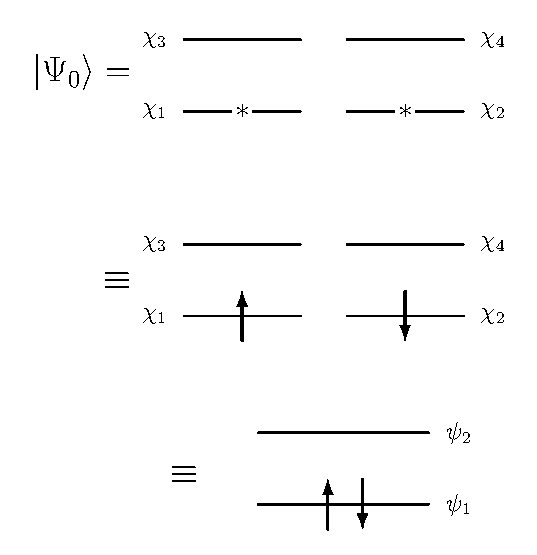
\includegraphics[width=0.55\textwidth]{H2}
  \caption{Closed-shell occupation of the spatial orbital in the minimal-basis
  description of \ce{H2}.}
  \label{fig:h2-closed-shell}
\end{figure}

The simple \ce{H2} example contains the entire logic needed for the general
closed-shell case: every occupied spatial orbital contributes twice to the
one-electron energy, Coulomb interactions occur between all spin
combinations, and exchange occurs only between same-spin electrons.

% ============================================================================
% General closed-shell determinant
% ============================================================================

\paragraph{General closed-shell determinant.}

Consider now a system containing an even number $N$ of electrons described
by a closed-shell RHF determinant. There are $N/2$ occupied spatial orbitals,
and each spatial orbital $\psi_i$ generates an $\alpha$ and a $\beta$ spin
orbital,
\begin{equation}
  \psi_i(\br)\alpha(\omega),
  \qquad
  \psi_i(\br)\beta(\omega).
\end{equation}

To avoid ambiguity, in the remainder of this derivation the indices
$i,j=1,\ldots,N/2$ label \emph{occupied spatial orbitals}, while
$\Bar{i}$ denotes the $\beta$ spin partner of spatial orbital $i$.

Starting from the general spin-orbital expression,
\begin{equation}
  \EHF
  =
  \sum_{p=1}^{N}\mel{p}{\hh}{p}
  +
  \frac{1}{2}
  \sum_{p=1}^{N}\sum_{q=1}^{N}
  \left[
    \braket{pq}{pq}
    -
    \braket{pq}{qp}
  \right],
  \label{eq:rhf-start-spin}
\end{equation}
we now sum explicitly over the two spin components associated with each
occupied spatial orbital.

\paragraph{One-electron contribution.}

The spin-orbital sum can be separated into its $\alpha$ and $\beta$
components:
\begin{align}
  \sum_{p=1}^{N}\mel{p}{\hh}{p}
  &=
  \sum_{i=1}^{N/2}\mel{i}{\hh}{i}
  +
  \sum_{i=1}^{N/2}\mel{\Bar{i}}{\hh}{\Bar{i}}
  \\
  &=
  \sum_{i=1}^{N/2}\rmel{i}{\hh}{i}
  +
  \sum_{i=1}^{N/2}\rmel{i}{\hh}{i}
  \\
  &=
  \boxed{
  2\sum_{i=1}^{N/2}\rmel{i}{\hh}{i}
  }.
  \label{eq:rhf-one-electron-spatial}
\end{align}
Again, the factor of two simply reflects the double occupation of every
occupied spatial orbital.

\paragraph{Two-electron contribution.}

For every pair of occupied spatial orbitals $i$ and $j$, four spin
combinations are possible:
\begin{equation}
  \alpha\alpha,
  \qquad
  \alpha\beta,
  \qquad
  \beta\alpha,
  \qquad
  \beta\beta.
\end{equation}
Separating these four possibilities gives
\begin{align}
  &\frac{1}{2}
  \sum_{p=1}^{N}\sum_{q=1}^{N}
  \left[
    \braket{pq}{pq}
    -
    \braket{pq}{qp}
  \right]
  \notag\\
  &\quad=
  \frac{1}{2}
  \Bigg\{
  \sum_{i=1}^{N/2}\sum_{j=1}^{N/2}
  \left(
    \braket{ij}{ij}
    -
    \braket{ij}{ji}
  \right)
  \notag\\
  &\qquad\quad+
  \sum_{i=1}^{N/2}\sum_{j=1}^{N/2}
  \left(
    \braket{\Bar{i}j}{\Bar{i}j}
    -
    \braket{\Bar{i}j}{j\Bar{i}}
  \right)
  \notag\\
  &\qquad\quad+
  \sum_{i=1}^{N/2}\sum_{j=1}^{N/2}
  \left(
    \braket{i\Bar{j}}{i\Bar{j}}
    -
    \braket{i\Bar{j}}{\Bar{j}i}
  \right)
  \notag\\
  &\qquad\quad+
  \sum_{i=1}^{N/2}\sum_{j=1}^{N/2}
  \left(
    \braket{\Bar{i}\Bar{j}}{\Bar{i}\Bar{j}}
    -
    \braket{\Bar{i}\Bar{j}}{\Bar{j}\Bar{i}}
  \right)
  \Bigg\}.
  \label{eq:rhf-four-spin-combinations}
\end{align}

The four Coulomb contributions all survive because they involve diagonal
spin overlaps. After integration over spin,
\begin{equation}
  \braket{ij}{ij}
  =
  \braket{\Bar{i}j}{\Bar{i}j}
  =
  \braket{i\Bar{j}}{i\Bar{j}}
  =
  \braket{\Bar{i}\Bar{j}}{\Bar{i}\Bar{j}}
  =
  \rbraket{ii}{jj}.
\end{equation}

Exchange behaves differently. The two same-spin combinations survive,
\begin{equation}
  \braket{ij}{ji}
  =
  \braket{\Bar{i}\Bar{j}}{\Bar{j}\Bar{i}}
  =
  \rbraket{ij}{ji},
\end{equation}
whereas the two opposite-spin exchange integrals vanish,
\begin{equation}
  \braket{\Bar{i}j}{j\Bar{i}}
  =
  \braket{i\Bar{j}}{\Bar{j}i}
  =
  0.
\end{equation}

For each pair of spatial orbitals, the four spin combinations therefore
produce
\begin{equation}
  \frac{1}{2}
  \left[
    4\rbraket{ii}{jj}
    -
    2\rbraket{ij}{ji}
  \right]
  =
  2\rbraket{ii}{jj}
  -
  \rbraket{ij}{ji}.
\end{equation}
Consequently,
\begin{equation}
  \boxed{
  \frac{1}{2}
  \sum_{p=1}^{N}\sum_{q=1}^{N}
  \left[
    \braket{pq}{pq}
    -
    \braket{pq}{qp}
  \right]
  =
  \sum_{i=1}^{N/2}\sum_{j=1}^{N/2}
  \left[
    2\rbraket{ii}{jj}
    -
    \rbraket{ij}{ji}
  \right]
  }.
  \label{eq:rhf-two-electron-spatial}
\end{equation}

Combining the one- and two-electron contributions gives the familiar
closed-shell RHF energy,
\begin{equation}
  \boxed{
  \EHF
  =
  2\sum_{i=1}^{N/2}
  \rmel{i}{\hh}{i}
  +
  \sum_{i=1}^{N/2}
  \sum_{j=1}^{N/2}
  \left[
    2\rbraket{ii}{jj}
    -
    \rbraket{ij}{ji}
  \right]
  }.
  \label{eq:rhf-energy-spatial}
\end{equation}

Introducing the spatial-orbital Coulomb and exchange integrals
\begin{equation}
  J_{ij}
  \equiv
  \rbraket{ii}{jj},
  \qquad
  K_{ij}
  \equiv
  \rbraket{ij}{ji},
\end{equation}
the same expression takes the compact form
\begin{equation}
  \boxed{
  \EHF
  =
  2\sum_{i=1}^{N/2}h_{ii}
  +
  \sum_{i=1}^{N/2}
  \sum_{j=1}^{N/2}
  \left(
    2J_{ij}-K_{ij}
  \right)
  }.
  \label{eq:rhf-energy-jk}
\end{equation}

The origin of the numerical factors is now transparent. Each occupied
spatial orbital contains two electrons, giving the factor of two in the
one-electron contribution. For each pair of spatial orbitals, all four spin
combinations contribute to the Coulomb interaction, whereas only the two
same-spin combinations contribute to exchange. After the overall factor
$1/2$ removing double counting, the result is precisely
\begin{equation}
  2J_{ij}-K_{ij}.
\end{equation}

Notice also that the terms with $i=j$ are perfectly well behaved:
\begin{equation}
  2J_{ii}-K_{ii}
  =
  J_{ii},
\end{equation}
since $J_{ii}=K_{ii}$. Thus, a doubly occupied spatial orbital contains one
physical Coulomb repulsion between its $\alpha$ and $\beta$ electrons; the
spurious same-spin self-interactions cancel through exchange.

% ============================================================================
% Open-shell examples
% ============================================================================

\paragraph{Problem: HF energy of the \ce{Li} atom.}

\violet{\textit{Find the HF energy of the \ce{Li} atom in terms of spatial
orbitals.}}

\paragraph{Solution.}

For the determinant considered here, the three occupied spin orbitals are
\begin{equation}
  \chi_1=\alpha\psi_1,
  \qquad
  \chi_2=\beta\psi_1,
  \qquad
  \chi_3=\alpha\psi_2.
\end{equation}
The first spatial orbital is therefore doubly occupied, whereas the second
contains a single $\alpha$ electron.

The one-electron contribution is immediately
\begin{equation}
  E_1
  =
  2h_{11}+h_{22}.
\end{equation}

There are three electron pairs. The two electrons in $\psi_1$ have opposite
spin and contribute
\begin{equation}
  J_{11}.
\end{equation}
The $\alpha$ electron in $\psi_2$ interacts Coulombically with both
electrons in $\psi_1$, giving
\begin{equation}
  2J_{12}.
\end{equation}
Exchange occurs only with the $\alpha$ electron in $\psi_1$, and therefore
contributes
\begin{equation}
  -K_{12}.
\end{equation}
The total energy is consequently
\begin{equation}
  \boxed{
  E_\text{HF}
  =
  2h_{11}
  +
  h_{22}
  +
  J_{11}
  +
  2J_{12}
  -
  K_{12}
  }.
\end{equation}

This example provides a useful way of reading spatial-orbital HF energies:
\red{Coulomb terms count interacting electron pairs, whereas exchange terms
count same-spin pairs}.

\paragraph{Problem: HF energy of the \ce{B} atom.}

\violet{\textit{Find the HF energy of the \ce{B} atom in terms of spatial
orbitals.}}

\paragraph{Solution.}

For the occupation considered here, the first two spatial orbitals are
doubly occupied and the third contains a single $\alpha$ electron,
corresponding schematically to
\begin{equation}
  \psi_1^2\psi_2^2\psi_3^1.
\end{equation}
The one-electron contribution is therefore
\begin{equation}
  E_1
  =
  2h_{11}
  +
  2h_{22}
  +
  h_{33}.
\end{equation}

The two electrons occupying $\psi_1$ contribute $J_{11}$, while those in
$\psi_2$ contribute $J_{22}$. Between the two doubly occupied orbitals there
are four Coulomb pairs but only two same-spin exchange pairs, giving
\begin{equation}
  4J_{12}-2K_{12}.
\end{equation}

The singly occupied $\psi_3$ orbital interacts with both electrons in each
doubly occupied orbital. Hence,
\begin{equation}
  2J_{13}-K_{13}
\end{equation}
arises from the interaction between $\psi_1$ and $\psi_3$, and
\begin{equation}
  2J_{23}-K_{23}
\end{equation}
from the interaction between $\psi_2$ and $\psi_3$.

Collecting all terms gives
\begin{equation}
  \boxed{
  \begin{split}
    E_\text{HF}
    ={}&
    2h_{11}
    +
    2h_{22}
    +
    h_{33}
    +
    J_{11}
    +
    4J_{12}
    +
    J_{22}
    -
    2K_{12}
    \\
    &+
    2J_{13}
    +
    2J_{23}
    -
    K_{13}
    -
    K_{23}.
  \end{split}
  }
\end{equation}

The \ce{Li} and \ce{B} examples illustrate that the reduction from spin
orbitals to spatial orbitals is not restricted to closed shells. The
closed-shell formula in Eq.~\eqref{eq:rhf-energy-spatial} benefits from the
particularly simple double-occupation pattern of RHF, but for a general
determinant the same procedure can always be carried out by keeping track of
which spatial orbitals are occupied by $\alpha$ and $\beta$ electrons.

The spatial-orbital representation is more compact, but the underlying
spin-orbital structure remains important. In particular, it determines
which exchange terms survive. This distinction will become useful in the
next section, where we consider determinants obtained by replacing occupied
spin orbitals with virtual ones.

\subsection{Excited determinants and Hamiltonian matrix elements}
\subsubsection{Excited determinants}

The Hartree--Fock solution provides not only an energy but also a complete
orthonormal set of occupied and virtual spin orbitals. Once this orbital basis
has been obtained, many other Slater determinants can be generated by
replacing one or more occupied spin orbitals of the HF determinant by virtual
ones. These determinants play a central role in configuration-interaction,
coupled-cluster, perturbation, and excited-state theories.

We therefore introduce the language of \red{orbital substitutions}, or
\red{excitations}, relative to the Hartree--Fock reference determinant.

\paragraph{Reference determinant.}

For a conventional ground-state HF solution, the electrons occupy the $N$
lowest spin orbitals according to the Aufbau principle. The reference
determinant is
\begin{equation}
  \boxed{
  \ket{\Psi_0}
  =
  \ket{
    \chi_1
    \ldots
    \chi_{\green{i}}
    \chi_{\green{j}}
    \ldots
    \chi_N
  }
  }.
  \label{eq:hf-reference-determinant}
\end{equation}
Here and in the following,
\begin{equation}
  \green{i,j,k,l,\ldots}
  \qquad\text{and}\qquad
  \red{a,b,c,d,\ldots}
\end{equation}
denote occupied and virtual spin orbitals, respectively.

The distinction is always made \emph{relative to the reference determinant}:
an occupied orbital contains an electron in $\ket{\Psi_0}$, whereas a virtual
orbital does not.

\begin{figure}[htbp]
  \centering
  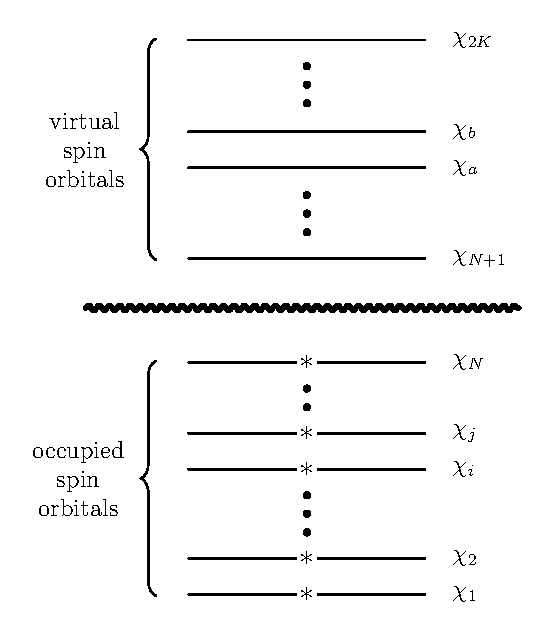
\includegraphics[width=0.34\textwidth]{HF_det}
  \caption{Reference Hartree--Fock determinant constructed from the occupied
  spin orbitals.}
  \label{fig:hf-reference-determinant}
\end{figure}

Because the spin orbitals form an orthonormal set, the occupied and virtual
subspaces are mutually orthogonal,
\begin{equation}
  \braket{\chi_i}{\chi_a}=0.
\end{equation}
This simple property will have important consequences for matrix elements
between different determinants.

% ============================================================================
% Single excitations
% ============================================================================

\paragraph{Singly excited determinants.}

A \red{singly excited determinant} is obtained by removing an electron from
an occupied spin orbital $i$ and placing it in a virtual spin orbital $a$.
Symbolically,
\begin{equation}
  \boxed{
  i\longrightarrow a
  }.
\end{equation}
The resulting determinant is denoted
\begin{equation}
  \ket{\Psi_{\green{i}}^{\red{a}}}.
\end{equation}
In determinant notation,
\begin{equation}
  \ket{\Psi_{\green{i}}^{\red{a}}}
  =
  \ket*{
    \chi_1
    \ldots
    \chi_{\red{a}}
    \chi_{\green{j}}
    \ldots
    \chi_N
  }.
\end{equation}
Thus, $\ket{\Psi_i^a}$ differs from the reference determinant by exactly one
spin orbital.

The same substitution can be expressed particularly compactly using
creation and annihilation operators,
\begin{equation}
  \boxed{
  \ket{\Psi_{\green{i}}^{\red{a}}}
  =
  \cre{\red{a}}
  \ani{\green{i}}
  \ket{\Psi_0}
  }.
  \label{eq:single-excited-determinant}
\end{equation}
The annihilation operator $\ani{i}$ first removes the electron occupying
spin orbital $i$, while the creation operator $\cre{a}$ places an electron
in the previously unoccupied spin orbital $a$.

It is useful to interpret this substitution as the simultaneous creation of
a \green{hole} in the occupied orbital $i$ and a \red{particle} in the
virtual orbital $a$:
\begin{equation}
  \boxed{
  i\rightarrow a
  \qquad\Longleftrightarrow\qquad
  \text{one hole }i
  +
  \text{one particle }a
  }.
\end{equation}
This particle-hole language will reappear naturally in excited-state and
many-body formulations.

Because one occupied orbital has been replaced by an orthogonal virtual
orbital,
\begin{equation}
  \boxed{
  \braket{\Psi_0}{\Psi_i^a}=0
  }.
\end{equation}
Thus, every singly excited determinant is orthogonal to the HF reference.

% ============================================================================
% Double excitations
% ============================================================================

\paragraph{Doubly excited determinants.}

A \red{doubly excited determinant} is obtained by replacing two occupied
spin orbitals, $i$ and $j$, by two virtual spin orbitals, $a$ and $b$:
\begin{equation}
  \boxed{
  ij\longrightarrow ab
  }.
\end{equation}
In determinant notation,
\begin{equation}
  \ket*{\Psi_{\green{ij}}^{\red{ab}}}
  =
  \ket{
    \chi_1
    \ldots
    \chi_{\red{a}}
    \chi_{\red{b}}
    \ldots
    \chi_N
  }.
\end{equation}
In second-quantized notation,
\begin{equation}
  \boxed{
  \ket*{\Psi_{\green{ij}}^{\red{ab}}}
  =
  \cre{\red{a}}
  \cre{\red{b}}
  \ani{\green{j}}
  \ani{\green{i}}
  \ket{\Psi_0}
  }.
  \label{eq:double-excited-determinant}
\end{equation}
The determinant now differs from the reference by two spin orbitals and
contains two holes, $i$ and $j$, together with two particles, $a$ and $b$.

The ordering of the fermionic creation and annihilation operators matters:
interchanging two such operators changes the sign because
\begin{equation}
  \cre{p}\cre{q}
  =
  -\cre{q}\cre{p},
  \qquad
  \ani{p}\ani{q}
  =
  -\ani{q}\ani{p}.
\end{equation}
A consistent ordering convention therefore fixes the overall phase of each
excited determinant. This phase has no effect on diagonal expectation
values, but it is essential when evaluating off-diagonal matrix elements
between different determinants.

\begin{figure}[htbp]
  \centering
  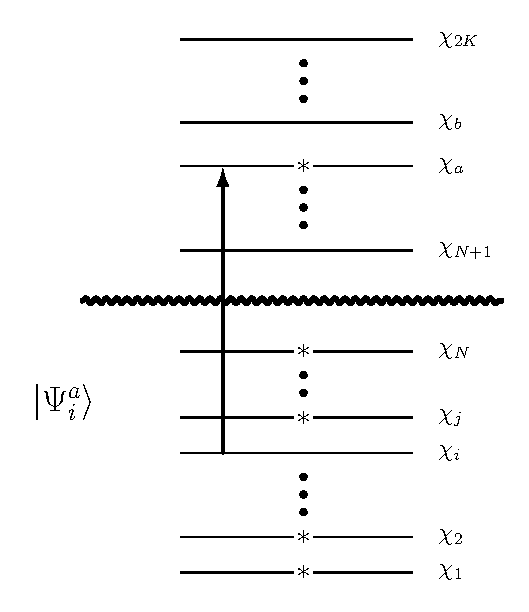
\includegraphics[width=0.25\textwidth]{single}
  \hspace{0.16\textwidth}
  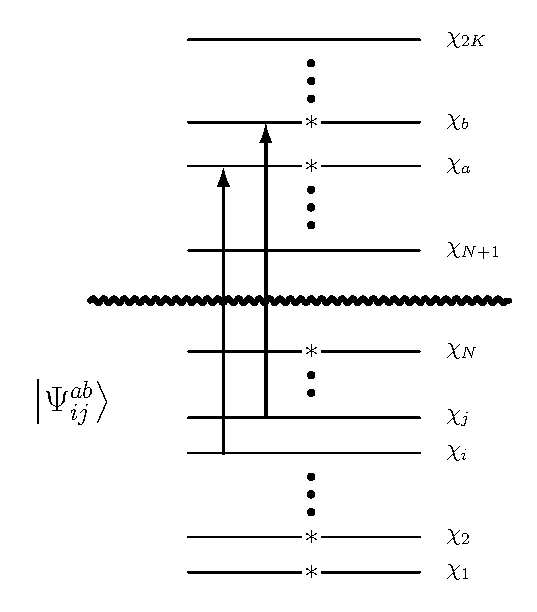
\includegraphics[width=0.25\textwidth]{double}
  \caption{Singly excited (left) and doubly excited (right) determinants
  obtained by replacing occupied spin orbitals of the Hartree--Fock
  reference by virtual ones.}
  \label{fig:excited-determinants}
\end{figure}

% ============================================================================
% Excitation rank
% ============================================================================

\paragraph{Excitation rank.}

The construction extends immediately to higher substitutions. A triple
excitation replaces three occupied orbitals,
\begin{equation}
  ijk\longrightarrow abc,
\end{equation}
and may be written
\begin{equation}
  \ket{\Psi_{ijk}^{abc}}
  =
  \cre{a}\cre{b}\cre{c}
  \ani{k}\ani{j}\ani{i}
  \ket{\Psi_0}.
\end{equation}
More generally, an $m$-fold excited determinant differs from the reference
by $m$ occupied-to-virtual substitutions. The integer $m$ is called the
\red{excitation rank}:
\begin{equation}
  \begin{array}{ccl}
    m=0 &:& \text{reference determinant},\\
    m=1 &:& \text{single excitation},\\
    m=2 &:& \text{double excitation},\\
    m=3 &:& \text{triple excitation},\\
    &\vdots&
  \end{array}
\end{equation}

With $N$ occupied spin orbitals and $2K-N$ virtual spin orbitals, the number
of singly excited determinants is
\begin{equation}
  N_\text{S}
  =
  N(2K-N),
\end{equation}
whereas the number of doubly excited determinants is
\begin{equation}
  N_\text{D}
  =
  \binom{N}{2}
  \binom{2K-N}{2}.
\end{equation}
The number of possible determinants therefore grows extremely rapidly with
the size of the orbital space. This combinatorial growth is one of the
fundamental computational difficulties encountered by correlated
wavefunction methods.

% ============================================================================
% Determinants versus excited states
% ============================================================================

\paragraph{Excited determinants are not necessarily excited states.}

An important distinction must be made at this point. The terminology
``singly excited determinant'' describes how a determinant is constructed
\emph{relative to the HF reference}; it does not imply that this determinant
is itself an eigenfunction of the electronic Hamiltonian.

In general,
\begin{equation}
  \chH_\text{elec}\ket{\Psi_i^a}
  \neq
  E_i^a\ket{\Psi_i^a},
\end{equation}
and similarly for doubly and higher excited determinants. The exact excited
states are, in general, linear combinations of many determinants,
\begin{equation}
  \ket{\Psi_I}
  =
  C_0^{(I)}\ket{\Psi_0}
  +
  \sum_{ia}
  C_i^{a,(I)}
  \ket{\Psi_i^a}
  +
  \frac{1}{4}
  \sum_{ijab}
  C_{ij}^{ab,(I)}
  \ket{\Psi_{ij}^{ab}}
  +
  \cdots.
\end{equation}
The determinants introduced here should therefore be viewed as a convenient
many-electron basis built from the HF orbitals.

This distinction is central to post-Hartree--Fock theory: the reference and
its excited determinants provide the building blocks, while the electronic
Hamiltonian determines how these configurations interact and combine.

% ============================================================================
% Connection to matrix elements
% ============================================================================

\paragraph{Why excitation rank matters.}

Two Slater determinants may differ by zero, one, two, or more spin orbitals.
For Hamiltonians containing only one- and two-electron operators, the matrix
element between two determinants depends very strongly on this number.

Schematically,
\begin{equation}
  \boxed{
  \text{number of orbital substitutions}
  \quad\Longrightarrow\quad
  \text{structure of the Hamiltonian matrix element}
  }.
\end{equation}
A one-electron operator can connect determinants differing by at most one
spin orbital, whereas a two-electron operator can connect determinants
differing by at most two. Consequently, determinants separated by three or
more substitutions have a vanishing Hamiltonian matrix element.

These selection rules are precisely the content of the
\red{Slater--Condon rules}, to which we now turn.

\subsubsection{Slater--Condon rules}

The determinants introduced in the previous subsection form an orthonormal
many-electron basis constructed from a common set of orthonormal spin
orbitals. The next question is therefore how the electronic Hamiltonian acts
in this determinant basis.

At first sight, evaluating a matrix element between two $N$-electron Slater
determinants might appear to require an explicit expansion of both
determinants into their $N!$ Hartree products. The
\red{Slater--Condon rules} avoid this combinatorial expansion. They express
matrix elements of one- and two-electron operators directly in terms of
one- and two-electron orbital integrals.

The central principle is simple: the value of a matrix element depends only
on the number of spin orbitals by which the two determinants differ. This
number is often called their \red{degree of substitution}. Because a
one-electron operator acts on only one electron at a time, it can connect
determinants differing by at most one spin orbital. Similarly, a
two-electron operator can connect determinants differing by at most two spin
orbitals.

Throughout this subsection, we assume that the determinants are written
with a consistent orbital ordering so that their relative fermionic phase
has already been fixed.

% ============================================================================
% One-electron operator
% ============================================================================

\paragraph{One-electron operators.}

Consider a general one-electron operator,
\begin{equation}
  \boxed{
  \chO_1
  =
  \sum_{p=1}^{N}\hh(\bx_p)
  }.
  \label{eq:slater-condon-one-body}
\end{equation}
The Slater--Condon rule depends on how many spin orbitals differ between the
two determinants.

\paragraph{Case 1: determinants differ by zero spin orbitals.}

If the two determinants are identical,
\begin{equation}
  \ket{\red{K}}
  =
  \ket{\cdots i j\cdots},
\end{equation}
then the matrix element is simply the sum of the one-electron expectation
values over all occupied spin orbitals:
\begin{equation}
  \boxed{
  \mel{\red{K}}{\chO_1}{\red{K}}
  =
  \sum_{i\in K}\mel{i}{\hh}{i}
  }.
  \label{eq:sc-one-zero}
\end{equation}
For the Hartree--Fock reference,
\begin{equation}
  \mel{\Psi_0}{\chO_1}{\Psi_0}
  =
  \sum_{i=1}^{N}h_{ii}.
\end{equation}

This is the result already encountered in the derivation of the HF energy:
each occupied spin orbital contributes one diagonal matrix element of the
one-electron operator.

\paragraph{Case 2: determinants differ by one spin orbital.}

Consider
\begin{equation}
  \ket{\red{K}}
  =
  \ket{\cdots i j\cdots},
  \qquad
  \ket{\blue{L}}
  =
  \ket{\cdots k j\cdots}.
\end{equation}
All occupied spin orbitals are common to the two determinants except for the
replacement
\begin{equation}
  i\longleftrightarrow k.
\end{equation}
The spectator orbitals integrate to unity, while orthogonality eliminates
all terms in which the one-electron operator acts on a common orbital.
Consequently,
\begin{equation}
  \boxed{
  \mel{\red{K}}{\chO_1}{\blue{L}}
  =
  \mel{i}{\hh}{k}
  }.
  \label{eq:sc-one-one}
\end{equation}
For example, between the HF reference and a singly excited determinant,
\begin{equation}
  \boxed{
  \mel*{\Psi_0}{\chO_1}{\Psi_{\green{i}}^{\red{a}}}
  =
  h_{\green{i}\red{a}}
  }.
\end{equation}

Thus a one-electron operator can directly remove an electron from one spin
orbital and place it in another.

\paragraph{Case 3: determinants differ by two or more spin orbitals.}

Let
\begin{equation}
  \ket{\red{K}}
  =
  \ket{\cdots i j\cdots},
  \qquad
  \ket{\blue{L}}
  =
  \ket{\cdots k l\cdots},
\end{equation}
so that at least two occupied spin orbitals differ. Since $\chO_1$ can act
on only one electron, it cannot simultaneously repair both substitutions.
At least one overlap between different orthogonal spin orbitals therefore
remains, and the matrix element vanishes:
\begin{equation}
  \boxed{
  \mel{\red{K}}{\chO_1}{\blue{L}}
  =
  0
  }.
  \label{eq:sc-one-two}
\end{equation}
In particular,
\begin{equation}
  \mel*{\Psi_0}{\chO_1}
  {\Psi_{\green{ij}}^{\red{ab}}}
  =
  0.
\end{equation}

More generally,
\begin{equation}
  \boxed{
  \chO_1
  \quad\text{connects determinants differing by at most one spin orbital}.
  }
\end{equation}

% ============================================================================
% Two-electron operator
% ============================================================================

\paragraph{Two-electron operators.}

Consider now the electron-electron interaction,
\begin{equation}
  \boxed{
  \chO_2
  =
  \sum_{p<q}^{N}\frac{1}{r_{pq}}
  }.
  \label{eq:slater-condon-two-body}
\end{equation}
Because this operator acts simultaneously on two electrons, its connectivity
extends one excitation rank further than that of a one-electron operator.

\paragraph{Case 1: determinants differ by zero spin orbitals.}

For identical determinants,
\begin{equation}
  \boxed{
  \mel{\red{K}}{\chO_2}{\red{K}}
  =
  \frac{1}{2}
  \sum_{i\in K}\sum_{j\in K}
  \mel{ij}{}{ij}
  }.
  \label{eq:sc-two-zero}
\end{equation}
The antisymmetrized integral
\begin{equation}
  \mel{ij}{}{ij}
  =
  \braket{ij}{ij}
  -
  \braket{ij}{ji}
\end{equation}
contains the Coulomb and exchange contributions associated with the occupied
pair $(i,j)$. The factor $1/2$ removes the double counting of electron
pairs.

For the HF reference,
\begin{equation}
  \boxed{
  \mel*{\Psi_0}{\chO_2}{\Psi_0}
  =
  \frac{1}{2}
  \sum_{ij}^{N}
  \mel{ij}{}{ij}
  }.
\end{equation}

\paragraph{Case 2: determinants differ by one spin orbital.}

Consider again
\begin{equation}
  \ket{\red{K}}
  =
  \ket{\cdots i j\cdots},
  \qquad
  \ket{\blue{L}}
  =
  \ket{\cdots k j\cdots}.
\end{equation}
One electron undergoes the substitution $i\rightarrow k$, while the second
electron acted upon by $\chO_2$ may occupy any spin orbital common to the two
determinants. Summing over these spectator occupied orbitals gives
\begin{equation}
  \boxed{
  \mel{\red{K}}{\chO_2}{\blue{L}}
  =
  \sum_{j\in K\cap L}
  \mel{ij}{}{kj}
  }.
  \label{eq:sc-two-one}
\end{equation}
For the reference and a singly excited determinant,
\begin{equation}
  \boxed{
  \mel*{\Psi_0}{\chO_2}
  {\Psi_{\green{i}}^{\red{a}}}
  =
  \sum_{k}^{N}
  \mel{\green{i}k}{}{\red{a}k}
  }.
  \label{eq:sc-reference-single-two-body}
\end{equation}

Physically, the promoted electron is coupled through the two-electron
interaction to each of the remaining occupied electrons.

\paragraph{Case 3: determinants differ by two spin orbitals.}

Let
\begin{equation}
  \ket{\red{K}}
  =
  \ket{\cdots i j\cdots},
  \qquad
  \ket{\blue{L}}
  =
  \ket{\cdots k l\cdots}.
\end{equation}
The two-electron operator can now act precisely on the two orbitals that
differ, giving
\begin{equation}
  \boxed{
  \mel{\red{K}}{\chO_2}{\blue{L}}
  =
  \mel{ij}{}{kl}
  }.
  \label{eq:sc-two-two}
\end{equation}
Thus,
\begin{equation}
  \boxed{
  \mel*{\Psi_0}{\chO_2}
  {\Psi_{\green{ij}}^{\red{ab}}}
  =
  \mel{\green{ij}}{}{\red{ab}}
  }.
\end{equation}

This result is particularly important in correlated wavefunction theory:
the two-electron interaction couples the HF reference directly to doubly
excited determinants.

\paragraph{Case 4: determinants differ by three or more spin orbitals.}

A two-electron operator cannot change three independent orbital occupations
simultaneously. Therefore,
\begin{equation}
  \boxed{
  \mel{\red{K}}{\chO_2}{\blue{L}}
  =
  0
  \qquad
  \text{if $K$ and $L$ differ by three or more spin orbitals}.
  }
  \label{eq:sc-two-three}
\end{equation}

Hence,
\begin{equation}
  \boxed{
  \chO_2
  \quad\text{connects determinants differing by at most two spin orbitals}.
  }
\end{equation}

% ============================================================================
% Full Hamiltonian
% ============================================================================

\paragraph{Slater--Condon rules for the electronic Hamiltonian.}

Because
\begin{equation}
  \chH_\text{elec}
  =
  \chO_1+\chO_2,
\end{equation}
the preceding results may be summarized directly for the electronic
Hamiltonian.

For identical determinants,
\begin{equation}
  \boxed{
  \mel{K}{\chH_\text{elec}}{K}
  =
  \sum_{i\in K}h_{ii}
  +
  \frac{1}{2}
  \sum_{i,j\in K}
  \mel{ij}{}{ij}
  }.
  \label{eq:sc-h-zero}
\end{equation}

For determinants differing by a single substitution $i\rightarrow a$,
\begin{equation}
  \boxed{
  \mel{\Psi_0}{\chH_\text{elec}}{\Psi_i^a}
  =
  h_{ia}
  +
  \sum_{k}^{N}
  \mel{ik}{}{ak}
  }.
  \label{eq:sc-h-single}
\end{equation}

For determinants differing by a double substitution $ij\rightarrow ab$,
\begin{equation}
  \boxed{
  \mel{\Psi_0}{\chH_\text{elec}}{\Psi_{ij}^{ab}}
  =
  \mel{ij}{}{ab}
  }.
  \label{eq:sc-h-double}
\end{equation}

Finally,
\begin{equation}
  \boxed{
  \mel{\Psi_0}{\chH_\text{elec}}{\Psi_{ijk}^{abc}}
  =
  0
  }
\end{equation}
and similarly for all higher excitation ranks.

The Hamiltonian matrix in a determinant basis is therefore highly
structured rather than dense: two determinants can interact directly only
if they differ by at most two spin orbitals. This sparsity is a direct
consequence of the fact that the nonrelativistic electronic Hamiltonian
contains at most two-electron operators.

% ============================================================================
% Excited determinant versus excited-state HF
% ============================================================================

\paragraph{Excited determinant versus excited HF solution.}

The terminology ``excited determinant'' must be distinguished carefully from
a separately optimized excited-state Hartree--Fock solution.

An excited determinant is
\begin{itemize}
  \item[\cmark] an orbital substitution within a \red{fixed} set of reference
    orbitals;
  \item[\cmark] a valid many-electron basis function;
  \item[\cmark] a building block for configuration-interaction and
    coupled-cluster expansions.
\end{itemize}
In general, an excited determinant is \emph{not necessarily}
\begin{itemize}
  \item[\xmark] a separately optimized HF state;
  \item[\xmark] a stationary point of the HF energy;
  \item[\xmark] an eigenfunction of $\chS^2$.
\end{itemize}
Thus,
\begin{equation}
  \boxed{
  \text{\red{orbital excitation}}
  \neq
  \text{\red{state-specific orbital optimization}}
  }.
\end{equation}

In the first procedure, the reference orbitals remain frozen and only their
occupation pattern changes. In the second, the orbitals themselves are
reoptimized for the targeted electronic state. The distinction is important
because orbital relaxation can be substantial, particularly for states with
a qualitatively different electronic distribution from the ground state.

% ============================================================================
% Brillouin
% ============================================================================

\paragraph{Brillouin's theorem.}

For a reference and a singly excited determinant, the Slater--Condon rules
give
\begin{align}
  \mel{\Psi_0}{\chH_\text{elec}}{\Psi_i^a}
  &=
  h_{ia}
  +
  \sum_{k}^{N}
  \mel{ik}{}{ak}.
\end{align}
The right-hand side is precisely an occupied-virtual matrix element of the
Fock operator,
\begin{equation}
  f_{ia}
  =
  h_{ia}
  +
  \sum_{k}^{N}
  \mel{ik}{}{ak}.
\end{equation}

At a stationary Hartree--Fock solution, occupied-virtual orbital rotations
cannot lower the energy to first order. The corresponding Fock matrix
elements therefore vanish:
\begin{equation}
  f_{ia}=0.
\end{equation}
Hence,
\begin{equation}
  \boxed{
  \mel{\Psi_0}{\chH_\text{elec}}
  {\Psi_{\green{i}}^{\red{a}}}
  =
  h_{\green{i}\red{a}}
  +
  \sum_{k}^{N}
  \mel{\green{i}k}{}{\red{a}k}
  =
  f_{\green{i}\red{a}}
  =
  0
  }.
  \label{eq:brillouin-theorem}
\end{equation}
This result is \red{Brillouin's theorem}.

Brillouin's theorem does not state that singly excited determinants are
unimportant. Rather, it states that a \emph{stationary HF determinant does
not couple directly to singles through the Hamiltonian}. This has several
important consequences. For example, single excitations do not contribute
directly to the ground-state correlation energy at first order around a
canonical HF reference, although they can enter indirectly through coupling
to other configurations.

The theorem also provides a useful physical interpretation of HF
stationarity: the orbitals have already been optimized so that infinitesimal
occupied-virtual mixing produces no first-order lowering of the energy.

% ============================================================================
% Spin
% ============================================================================

\paragraph{Spin quantum numbers.}

Excited determinants also provide a useful setting in which to distinguish
the spin projection $M_S$ from the total spin $S$.

Within the nonrelativistic spin-free framework, the electronic Hamiltonian
commutes with both the total-spin operator and its projection along the
chosen quantization axis,
\begin{equation}
  \boxed{
  \comm{\chH}{\purple{\chS^2}}=0,
  \qquad
  \comm{\chH}{\violet{\chS_z}}=0
  }.
\end{equation}
The exact eigenfunctions of $\chH$ may therefore be chosen as simultaneous
eigenfunctions of $\chS^2$ and $\chS_z$:
\begin{align}
  \purple{\chS^2}\ket{S,M_S}
  &=
  S(S+1)\ket{S,M_S},
  \\
  \violet{\chS_z}\ket{S,M_S}
  &=
  M_S\ket{S,M_S}.
\end{align}

The quantum number $S$ determines the \purple{spin multiplicity},
\begin{equation}
  \boxed{
  \text{multiplicity}=2S+1
  }.
\end{equation}
Thus,
\begin{equation}
  S=0,\quad\frac{1}{2},\quad1,\quad\frac{3}{2},\ldots
\end{equation}
correspond to singlets, doublets, triplets, quartets, and so forth. For a
given value of $S$, the spin projection takes the values
\begin{equation}
  M_S=-S,-S+1,\ldots,S-1,S.
\end{equation}

For a collinear determinant containing $N^\alpha$ spin-up and $N^\beta$
spin-down electrons,
\begin{equation}
  \boxed{
  \violet{\chS_z}\ket{\Psi}
  =
  M_S\ket{\Psi},
  \qquad
  M_S
  =
  \frac{N^\alpha-N^\beta}{2}
  }.
  \label{eq:ms-determinant}
\end{equation}
Here, \emph{collinear} means that all occupied spin orbitals are expressed
with respect to the same spin quantization axis.

Every RHF or collinear UHF determinant therefore has a definite value of
$M_S$. Having a definite $M_S$, however, does \emph{not} imply having a
definite total spin $S$.

\paragraph{Closed-shell RHF.}

For a closed-shell RHF determinant,
\begin{equation}
  N^\alpha=N^\beta=\frac{N}{2},
  \qquad
  M_S=0.
\end{equation}
Because every spatial orbital is occupied by one $\alpha$ and one $\beta$
electron, the determinant is a pure singlet:
\begin{equation}
  \boxed{
  \purple{\chS^2}\ket{\Psi_\text{RHF}}
  =
  0
  }.
\end{equation}

Thus, a closed-shell RHF determinant is simultaneously an eigenfunction of
$\chS_z$ and $\chS^2$.

\paragraph{Open-shell UHF.}

For UHF, the $\alpha$ and $\beta$ electrons are allowed to occupy different
spatial orbitals. The determinant remains an eigenfunction of $\chS_z$, but,
in general,
\begin{equation}
  \purple{\chS^2}\ket{\Psi_\text{UHF}}
  \neq
  S(S+1)\ket{\Psi_\text{UHF}}.
\end{equation}
Hence,
\begin{equation}
  \boxed{
  \text{every collinear RHF or UHF determinant has definite $M_S$, but
  only special determinants have definite $S$}.
  }
\end{equation}

For $N^\alpha\geq N^\beta$, the expectation value of $\chS^2$ for a UHF
determinant is
\begin{equation}
  \boxed{
  \expval{\purple{\chS^2}}_\text{UHF}
  =
  M_S(M_S+1)
  +
  N^\beta
  -
  \sum_{i=1}^{N^\alpha}
  \sum_{j=1}^{N^\beta}
  \abs{S_{ij}^{\alpha\beta}}^2
  },
  \qquad
  \underbrace{
  S_{ij}^{\alpha\beta}
  }_{\text{overlap}}
  =
  \braket{\psi_i^\alpha}{\psi_j^\beta}.
  \label{eq:uhf-spin-contamination}
\end{equation}

If the $\alpha$ and $\beta$ spatial orbitals coincide pairwise, the overlap
terms take their maximal values and the spin-pure restricted result is
recovered. As the two spin manifolds relax independently, the value of
$\expval{\chS^2}$ may depart from the desired eigenvalue.

For a target high-spin state with
\begin{equation}
  S=M_S,
\end{equation}
the spin contamination may be quantified as
\begin{equation}
  \boxed{
  \Delta S^2
  =
  \expval{\purple{\chS^2}}_\text{UHF}
  -
  \expval{\purple{\chS^2}}_\text{exact}
  \geq0
  }.
\end{equation}
More explicitly,
\begin{itemize}
  \item a singlet may be contaminated by triplets, quintets, $\ldots$;
  \item a doublet may be contaminated by quartets, sextets, $\ldots$;
  \item a triplet may be contaminated by quintets, septets, $\ldots$;
  \item restoring spin symmetry generally requires \red{spin projection} or
    \red{a linear combination of determinants}.
\end{itemize}

The last point is particularly important: a linear combination of
determinants can possess a well-defined total spin even when the individual
determinants do not.

% ============================================================================
% Spin adaptation
% ============================================================================

\paragraph{Spin adaptation of singly excited determinants.}

Consider a closed-shell singlet reference and promote one electron from the
doubly occupied spatial orbital $i$ to the virtual spatial orbital $a$.
There are two distinct $M_S=0$ determinants,
\begin{equation}
  \boxed{
  \ket{D_\alpha}
  =
  \cre{a\alpha}\ani{i\alpha}\ket{\Psi_0},
  \qquad
  \ket{D_\beta}
  =
  \cre{a\beta}\ani{i\beta}\ket{\Psi_0}.
  }
  \label{eq:spin-adapted-determinants}
\end{equation}
The first promotes the $\alpha$ electron and leaves the $\beta$ electron in
orbital $i$, whereas the second promotes the $\beta$ electron.

Both determinants contain one $\alpha$ and one $\beta$ electron in the two
open-shell orbitals. Consequently,
\begin{equation}
  \violet{\chS_z}\ket{D_\sigma}
  =
  0,
\end{equation}
and each determinant has
\begin{equation}
  \mel{D_\sigma}{\purple{\chS^2}}{D_\sigma}
  =
  1.
\end{equation}
The value $1$ is neither the singlet eigenvalue $0$ nor the triplet
eigenvalue $2$. Therefore, neither determinant is individually an
eigenfunction of $\chS^2$.

\begin{center}
\begin{minipage}[t]{0.43\textwidth}
  \centering
  $\ket{D_\alpha}$: excite the spin-up electron

  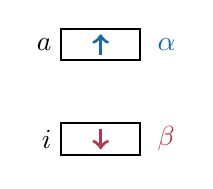
\begin{tikzpicture}[x=1cm,y=1cm]
    \node[left] at (0,0.35) {$i$};
    \node[left] at (0,1.55) {$a$};
    \draw[thick] (0,0.15) rectangle (1.0,0.55);
    \draw[thick] (0,1.35) rectangle (1.0,1.75);
    \draw[hfRed,very thick,->] (0.50,0.48)--(0.50,0.22);
    \draw[hfBlue,very thick,->] (0.50,1.42)--(0.50,1.68);
    \node[hfRed,right] at (1.10,0.35) {$\beta$};
    \node[hfBlue,right] at (1.10,1.55) {$\alpha$};
  \end{tikzpicture}
\end{minipage}
\hfill
\begin{minipage}[t]{0.43\textwidth}
  \centering
  $\ket{D_\beta}$: excite the spin-down electron

  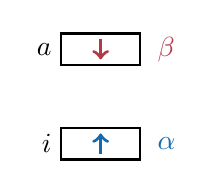
\begin{tikzpicture}[x=1cm,y=1cm]
    \node[left] at (0,0.35) {$i$};
    \node[left] at (0,1.55) {$a$};
    \draw[thick] (0,0.15) rectangle (1.0,0.55);
    \draw[thick] (0,1.35) rectangle (1.0,1.75);
    \draw[hfBlue,very thick,->] (0.50,0.22)--(0.50,0.48);
    \draw[hfRed,very thick,->] (0.50,1.68)--(0.50,1.42);
    \node[hfBlue,right] at (1.10,0.35) {$\alpha$};
    \node[hfRed,right] at (1.10,1.55) {$\beta$};
  \end{tikzpicture}
\end{minipage}
\end{center}

Each determinant has $M_S=0$, but contains equal singlet and triplet
character. This provides a concrete demonstration that being an eigenfunction
of $\violet{\chS_z}$ does not imply being an eigenfunction of
$\purple{\chS^2}$. In particular,
\begin{equation}
  \boxed{
  \text{\red{an open-shell determinant need not be a pure spin function}.}
  }
\end{equation}

In the determinant basis
\begin{equation}
  \left\{
  \ket{D_\alpha},
  \ket{D_\beta}
  \right\},
\end{equation}
the matrix representation of $\chS^2$ is
\begin{equation}
  \boxed{
  [\purple{\chS^2}]_{\{D_\alpha,D_\beta\}}
  =
  \begin{pmatrix}
    1 & -1\\
    -1 & 1
  \end{pmatrix}
  }.
\end{equation}
The determinant basis is therefore not spin adapted. Diagonalizing this
$2\times2$ matrix produces eigenvectors with definite values of $S$.

The symmetric combination has eigenvalue zero,
\begin{equation}
  \boxed{
  \ket{{}^1\Psi_i^a}
  =
  \frac{
    \ket{D_\alpha}
    \red{+}
    \ket{D_\beta}
  }{\sqrt{2}}
  },
  \qquad
  \purple{\chS^2}
  \ket{{}^1\Psi_i^a}
  =
  0,
\end{equation}
and is therefore a pure singlet,
\begin{equation}
  S=0.
\end{equation}

The antisymmetric combination has eigenvalue two,
\begin{equation}
  \boxed{
  \ket{{}^{3,0}\Psi_i^a}
  =
  \frac{
    \ket{D_\alpha}
    \red{-}
    \ket{D_\beta}
  }{\sqrt{2}}
  },
\end{equation}
with
\begin{equation}
  \purple{\chS^2}
  \ket{{}^{3,0}\Psi_i^a}
  =
  2
  \ket{{}^{3,0}\Psi_i^a},
\end{equation}
and therefore
\begin{equation}
  S=1.
\end{equation}
It is the $M_S=0$ component of a triplet.

Thus,
\begin{equation}
  \boxed{
  \text{\red{spin adaptation is the diagonalization of $\chS^2$
  in a determinant space}.}
  }
\end{equation}

\paragraph{Spatial and spin symmetry.}

The same result can be understood directly from the permutation symmetry of
the two open-shell electrons.

For two open-shell spatial orbitals $i$ and $a$, the singlet may be written
as
\begin{equation}
  \ket{{}^1\Psi_i^a}
  =
  \frac{1}{2}
  \underbrace{
  \qty[
    \ket{\phi_i(1)\phi_a(2)}
    +
    \ket{\phi_a(1)\phi_i(2)}
  ]}_{\text{spatially symmetric}}
  \underbrace{
  \qty[
    \alpha(1)\beta(2)
    -
    \beta(1)\alpha(2)
  ]}_{\text{spin antisymmetric}}.
\end{equation}
The spatial factor is \green{symmetric} under exchange of the two electrons,
whereas the spin factor is \red{antisymmetric}. Their product is therefore
antisymmetric, as required for fermions.

For the $M_S=0$ triplet,
\begin{equation}
  \ket{{}^{3,0}\Psi_i^a}
  =
  \frac{1}{2}
  \underbrace{
  \qty[
    \ket{\phi_i(1)\phi_a(2)}
    -
    \ket{\phi_a(1)\phi_i(2)}
  ]}_{\text{spatially antisymmetric}}
  \underbrace{
  \qty[
    \alpha(1)\beta(2)
    +
    \beta(1)\alpha(2)
  ]}_{\text{spin symmetric}}.
\end{equation}
Here the spatial factor is \red{antisymmetric} and the spin factor is
\green{symmetric}. Again,
\begin{equation}
  \boxed{
  \text{the total electronic wavefunction is antisymmetric}.
  }
\end{equation}

This complementary symmetry between spatial and spin parts is a direct
consequence of the Pauli principle introduced earlier in the chapter.

\paragraph{The three triplet components.}

A state with $S=1$ contains three components corresponding to
\begin{equation}
  M_S=+1,\quad0,\quad-1.
\end{equation}
For the two open-shell orbitals $i$ and $a$, these are
\begin{align}
  \ket{{}^{3,+1}\Psi_i^a}
  &=
  \ket{\cdots i^\alpha a^\alpha\cdots},
  &
  \ket{{}^{3,0}\Psi_i^a}
  &=
  \frac{\ket{D_\alpha}-\ket{D_\beta}}{\sqrt{2}},
  &
  \ket{{}^{3,-1}\Psi_i^a}
  &=
  \ket{\cdots i^\beta a^\beta\cdots}.
\end{align}
All three belong to the same spin multiplet and satisfy
\begin{equation}
  \purple{\chS^2}\ket{1,M_S}
  =
  2\ket{1,M_S},
  \qquad
  \violet{\chS_z}\ket{1,M_S}
  =
  M_S\ket{1,M_S}.
\end{equation}

The components are connected by the spin ladder operators,
\begin{equation}
  \boxed{
  \underbrace{
  \chS_\pm
  }_{\text{\red{ladder operator}}}
  \ket{S,M_S}
  =
  \sqrt{
    S(S+1)-M_S(M_S\pm1)
  }
  \ket{S,M_S\pm1}
  }.
\end{equation}
The $M_S=\pm1$ triplet components are each represented by a single
spin-pure determinant. By contrast, the $M_S=0$ component requires a linear
combination of two determinants.

This example illustrates a general lesson that will recur throughout
electronic-structure theory: determinants are a convenient antisymmetric
basis, but states with the correct physical symmetries often require
specific linear combinations of determinants.

\subsection{The Fock operator and orbital energies}
\subsubsection{The Fock operator}

The Hartree--Fock approximation has so far been formulated as an energy
functional of a set of orthonormal occupied spin orbitals,
\begin{equation}
  E_\text{HF}[\{\chi_i\}]
  =
  \sum_{i=1}^{N} h_{ii}
  +
  \frac{1}{2}
  \sum_{i=1}^{N}\sum_{j=1}^{N}
  \mel{ij}{}{ij}.
  \label{eq:hf-energy-orbital-functional}
\end{equation}
The Hartree--Fock problem consists in finding the set of spin orbitals that
makes this energy stationary while preserving their orthonormality,
\begin{equation}
  \braket{\chi_i}{\chi_j}
  =
  \delta_{ij}.
\end{equation}

This is a constrained variational problem. Since the orthonormality
conditions couple every pair of occupied spin orbitals, a single Lagrange
multiplier is not sufficient. Instead, one introduces a complete matrix of
multipliers $\bepsilon$ and defines the Hartree--Fock Lagrangian
\begin{equation}
  \boxed{
  \mathcal{L}[\{\chi_i\}]
  =
  E_\text{HF}[\{\chi_i\}]
  -
  \sum_{ij}
  \underbrace{\epsilon_{ji}}_{
    \substack{\text{\red{Lagrange}}\\
              \text{\red{multipliers}}}
  }
  \underbrace{
    \qty(
      \braket{\chi_i}{\chi_j}
      -
      \delta_{ij}
    )
  }_{
    \substack{\text{\green{orthonormality}}\\
              \text{\green{constraint}}}
  }
  }.
  \label{eq:hf-lagrangian}
\end{equation}

The orbitals and their complex conjugates may be treated as independent
variables in the variation. Stationarity with respect to
$\chi_i^*(\bx)$ requires
\begin{equation}
  \fdv{\mathcal{L}}{\chi_i^*(\bx)}
  =
  0.
  \label{eq:hf-stationarity}
\end{equation}

\paragraph{Functional derivative of the HF energy.}

The one-electron part is straightforward:
\begin{equation}
  \fdv{}{\chi_i^*(\bx)}
  \sum_j
  \mel{\chi_j}{\hh}{\chi_j}
  =
  \hh(\bx)\chi_i(\bx).
\end{equation}

The derivative of the two-electron contribution generates the Coulomb and
exchange operators. Using the symmetry of the double sum, the factor
$1/2$ disappears because the orbital $\chi_i$ may occur in either member
of an interacting pair:
\begin{equation}
  \fdv{}{\chi_i^*(\bx)}
  \left[
    \frac{1}{2}
    \sum_{jk}
    \mel{jk}{}{jk}
  \right]
  =
  \sum_{j=1}^{N}
  \left[
    \chJ_j(\bx)
    -
    \chK_j(\bx)
  \right]
  \chi_i(\bx).
\end{equation}

Consequently,
\begin{equation}
  \boxed{
  \fdv{E_\text{HF}}{\chi_i^*(\bx)}
  =
  \left\{
    \hh(\bx)
    +
    \sum_{j=1}^{N}
    \left[
      \chJ_j(\bx)-\chK_j(\bx)
    \right]
  \right\}
  \chi_i(\bx)
  }.
\end{equation}

This motivates the definition of the \red{Fock operator},
\begin{equation}
  \boxed{
  \hf(\bx)
  =
  \hh(\bx)
  +
  \underbrace{
    \sum_{j=1}^{N}
    \left[
      \chJ_j(\bx)-\chK_j(\bx)
    \right]
  }_{
    \Hat{v}^{\text{HF}}(\bx)
    \text{ = \red{Hartree--Fock potential}}
  }
  }.
  \label{eq:fock-operator}
\end{equation}

The Fock operator is therefore an effective one-electron operator composed
of the core Hamiltonian and the average interaction with all occupied spin
orbitals. The Coulomb term represents the classical electrostatic
interaction with the electronic distribution, whereas the exchange term is
a purely fermionic contribution arising from antisymmetry.

As discussed previously, the Coulomb operator is local while the exchange
operator is nonlocal. The Fock operator is therefore, in general, a
nonlocal one-electron operator.

Notice also that an electron does not interact with itself. When the Fock
operator acts on $\chi_i$,
\begin{equation}
  \left(
    \chJ_i-\chK_i
  \right)
  \ket{\chi_i}
  =
  0,
\end{equation}
because the Coulomb and exchange self-interaction contributions are
identical and cancel exactly.

\paragraph{The Hartree--Fock equations.}

Taking the functional derivative of the constraint term in
Eq.~\eqref{eq:hf-lagrangian} gives
\begin{equation}
  \fdv{}{\chi_i^*(\bx)}
  \sum_{jk}
  \epsilon_{kj}
  \braket{\chi_j}{\chi_k}
  =
  \sum_j
  \epsilon_{ji}
  \chi_j(\bx).
\end{equation}
The stationarity condition therefore becomes
\begin{equation}
  \boxed{
  \hf(\bx)\chi_i(\bx)
  =
  \sum_j
  \epsilon_{ji}\chi_j(\bx)
  }.
  \label{eq:general-hf-equations}
\end{equation}

These are the general Hartree--Fock equations. An important feature is that
the Fock operator acting on a given occupied spin orbital need not return
that same orbital. It is only required to remain within the space spanned
by the occupied spin orbitals.

Multiplying Eq.~\eqref{eq:general-hf-equations} from the left by
$\bra{\chi_k}$ and using orthonormality gives
\begin{equation}
  \epsilon_{ki}
  =
  \mel{\chi_k}{\hf}{\chi_i}.
  \label{eq:lagrange-fock}
\end{equation}
Since $\hf$ is Hermitian,
\begin{equation}
  \mel{\chi_k}{\hf}{\chi_i}
  =
  \mel{\chi_i}{\hf}{\chi_k}^*,
\end{equation}
and hence
\begin{equation}
  \boxed{
  \epsilon_{ki}
  =
  \epsilon_{ik}^*
  }.
\end{equation}
The matrix of Lagrange multipliers is therefore Hermitian,
\begin{equation}
  \boxed{
  \bepsilon^\dag=\bepsilon
  }.
\end{equation}

This property is crucial because every Hermitian matrix can be diagonalized
by a unitary transformation.

\paragraph{Why the HF equations are self-consistent.}

Equation~\eqref{eq:general-hf-equations} resembles an ordinary one-electron
eigenvalue problem, but there is a fundamental difference. The Fock
operator itself depends on the occupied orbitals through the Coulomb and
exchange operators:
\begin{equation}
  \boxed{
  \hf
  =
  \hf[\chi_1,\chi_2,\ldots,\chi_N]
  }.
\end{equation}
The orbitals are therefore required to satisfy an equation containing an
operator constructed from those same orbitals.

Schematically,
\begin{equation}
  \boxed{
  \{\chi_i\}
  \quad\longrightarrow\quad
  \hf[\{\chi_i\}]
  \quad\longrightarrow\quad
  \{\chi_i\}
  }.
\end{equation}
The Hartree--Fock equations are consequently \red{nonlinear} and must be
solved self-consistently. This is the origin of the term
\red{self-consistent field} (SCF).

In practice, one starts from a trial set of orbitals, constructs the
corresponding Fock operator, obtains a new set of orbitals, and repeats the
procedure until the orbitals, density, and energy are self-consistent.

The variational equations establish a stationary point of the HF energy.
They do not, by themselves, guarantee that a particular SCF solution is the
global minimum: multiple HF stationary solutions may exist.

\paragraph{Unitary invariance of the occupied orbitals.}

The HF determinant is not associated with a unique set of occupied
orbitals. Consider a unitary transformation among the occupied spin
orbitals,
\begin{equation}
  \boxed{
  \widetilde{\chi}_i(\bx)
  =
  \sum_j
  \chi_j(\bx)
  \purple{U}_{ji}
  },
  \qquad
  \purple{\bU}^\dag\cdot\purple{\bU}
  =
  \bI.
  \label{eq:occupied-unitary-rotation}
\end{equation}
The transformed orbitals remain orthonormal:
\begin{align}
  \braket{\widetilde{\chi}_i}{\widetilde{\chi}_j}
  &=
  \sum_{kl}
  U_{ki}^*
  U_{lj}
  \braket{\chi_k}{\chi_l}
  \\
  &=
  \sum_k
  U_{ki}^*U_{kj}
  =
  \delta_{ij}.
\end{align}

More importantly, the occupied one-particle projector is unchanged:
\begin{align}
  \sum_i
  \widetilde{\chi}_i(\bx)
  \widetilde{\chi}_i^*(\bx')
  &=
  \sum_{ijk}
  \chi_j(\bx)
  U_{ji}
  U_{ki}^*
  \chi_k^*(\bx')
  \\
  &=
  \sum_{jk}
  \chi_j(\bx)
  \delta_{jk}
  \chi_k^*(\bx')
  \\
  &=
  \sum_j
  \chi_j(\bx)
  \chi_j^*(\bx').
\end{align}
Since the Fock operator depends only on the occupied one-particle density,
it is invariant under this transformation.

The determinant itself transforms as
\begin{equation}
  \boxed{
  \ket*{\widetilde{\Psi}_\text{HF}}
  =
  \det(\purple{\bU})
  \ket*{\Psi_\text{HF}}
  }.
  \label{eq:det-unitary-transform}
\end{equation}
Because $\purple{\bU}$ is unitary,
\begin{equation}
  \purple{\bU}^{\dag}\cdot\purple{\bU}
  =
  \bI
  \quad\Rightarrow\quad
  \det(
    \purple{\bU}^{\dag}\cdot\purple{\bU}
  )
  =
  1,
\end{equation}
and therefore
\begin{equation}
  \abs{\det(\purple{\bU})}^2
  =
  1
  \quad\Rightarrow\quad
  \det(\purple{\bU})
  =
  e^{\ii\theta}.
\end{equation}
Hence,
\begin{equation}
  \boxed{
  \ket*{\widetilde{\Psi}_\text{HF}}
  =
  e^{\ii\theta}
  \ket*{\Psi_\text{HF}}
  }.
\end{equation}
The two determinants differ only by an irrelevant global phase and describe
the same physical state.

Thus,
\begin{equation}
  \boxed{
  \text{unitary rotations within the occupied space leave
  $E_\text{HF}$ and $\Psi_\text{HF}$ unchanged}.
  }
\end{equation}

\paragraph{Canonical Hartree--Fock orbitals.}

This unitary freedom can be exploited to choose a particularly convenient
set of occupied orbitals. Since the Lagrange-multiplier matrix is Hermitian,
there exists a unitary matrix $\purple{\bU}$ such that
\begin{equation}
  \boxed{
  \widetilde{\bepsilon}
  =
  \purple{\bU}^{\dag}
  \cdot
  \bepsilon
  \cdot
  \purple{\bU}
  }
\end{equation}
is diagonal:
\begin{equation}
  \widetilde{\epsilon}_{ij}
  =
  \epsilon_i\delta_{ij}.
\end{equation}

Applying the same unitary transformation to the occupied orbitals converts
the general HF equations,
\begin{equation}
  \hf\ket{\chi_i}
  =
  \sum_j
  \epsilon_{ji}\ket{\chi_j},
\end{equation}
into
\begin{equation}
  \hf\ket{\widetilde{\chi}_i}
  =
  \epsilon_i
  \ket{\widetilde{\chi}_i}.
\end{equation}
Dropping the tildes, one obtains the
\red{canonical Hartree--Fock equations},
\begin{equation}
  \boxed{
  \hf(\bx)\chi_i(\bx)
  =
  \epsilon_i\chi_i(\bx)
  }.
  \label{eq:canonical-hf}
\end{equation}
The eigenfunctions $\{\chi_i\}$ are called
\red{canonical spin orbitals}, and the corresponding eigenvalues
$\{\epsilon_i\}$ are called \red{orbital energies}.

Canonicalization does not produce a new Hartree--Fock wavefunction. It is
only a convenient choice of basis within the same occupied orbital space.

At self-consistency, the Fock operator may also be diagonalized in the
orthogonal complement of the occupied space. This defines the
\red{canonical virtual orbitals}. The complete canonical orbital set then
satisfies
\begin{equation}
  \boxed{
  \mel{\chi_p}{\hf}{\chi_q}
  =
  \epsilon_p\delta_{pq}
  }.
  \label{eq:canonical-fock-diagonal}
\end{equation}

In particular, the occupied-virtual block vanishes,
\begin{equation}
  \boxed{
  f_{ia}
  =
  \mel{i}{\hf}{a}
  =
  0
  }.
  \label{eq:occupied-virtual-fock-zero}
\end{equation}
This is the orbital form of the stationarity condition encountered in
Brillouin's theorem:
\begin{equation}
  \mel{\Psi_0}{\chH_\text{elec}}{\Psi_i^a}
  =
  f_{ia}
  =
  0.
\end{equation}

% ============================================================================
% Fock matrix elements
% ============================================================================

\paragraph{Problem: Fock matrix elements in the spin-orbital basis.}

\violet{\textit{Find the expression of the matrix elements
\[
  f_{ij}
  =
  \mel{\chi_i}{\hf}{\chi_j}.
\]
}}

\paragraph{Solution.}

Expanding the Fock operator gives
\begin{align}
  f_{ij}
  &=
  \mel{\chi_i}
      {
        \hh
        +
        \sum_k
        \qty(
          \chJ_k-\chK_k
        )
      }
      {\chi_j}
  \\
  &=
  \mel{\chi_i}{\hh}{\chi_j}
  +
  \sum_k
  \left[
    \mel{\chi_i}{\chJ_k}{\chi_j}
    -
    \mel{\chi_i}{\chK_k}{\chi_j}
  \right].
\end{align}

The Coulomb contribution is
\begin{equation}
  \mel{\chi_i}{\chJ_k}{\chi_j}
  =
  \braket{ik}{jk},
\end{equation}
whereas the exchange contribution is
\begin{equation}
  \mel{\chi_i}{\chK_k}{\chi_j}
  =
  \braket{ik}{kj}.
\end{equation}
Therefore,
\begin{align}
  f_{ij}
  &=
  \mel{i}{\hh}{j}
  +
  \sum_k
  \left[
    \braket{ik}{jk}
    -
    \braket{ik}{kj}
  \right]
  \\
  &=
  \boxed{
  \mel{i}{\hh}{j}
  +
  \sum_k
  \mel{ik}{}{jk}
  }.
  \label{eq:fock-matrix-spin-orbital}
\end{align}

Thus, each Fock matrix element contains the bare one-electron contribution
plus the Coulomb and exchange interactions with all occupied spin orbitals.

For an occupied-virtual matrix element,
\begin{equation}
  f_{ia}
  =
  h_{ia}
  +
  \sum_k
  \mel{ik}{}{ak},
\end{equation}
which is precisely the quantity appearing in Brillouin's theorem.

% ============================================================================
% Orbital energies
% ============================================================================

\paragraph{Problem: orbital energies in the spin-orbital basis.}

\violet{\textit{Deduce the expression of $\epsilon_i$.}}

\paragraph{Solution.}

For a canonical orbital,
\begin{equation}
  \hf\ket{\chi_i}
  =
  \epsilon_i\ket{\chi_i}.
\end{equation}
Multiplying by $\bra{\chi_i}$ gives
\begin{align}
  \mel{\chi_i}{\hf}{\chi_i}
  &=
  \epsilon_i
  \braket{\chi_i}{\chi_i}
  \\
  &=
  \epsilon_i,
\end{align}
because the orbital is normalized. Therefore,
\begin{align}
  \epsilon_i
  &=
  f_{ii}
  \\
  &=
  \mel{i}{\hh}{i}
  +
  \sum_k
  \left[
    \braket{ik}{ik}
    -
    \braket{ik}{ki}
  \right]
  \\
  &=
  \boxed{
  \mel{i}{\hh}{i}
  +
  \sum_k
  \mel{ik}{}{ik}
  }.
  \label{eq:hf-orbital-energy}
\end{align}

The term with $k=i$ vanishes,
\begin{equation}
  \mel{ii}{}{ii}
  =
  \braket{ii}{ii}
  -
  \braket{ii}{ii}
  =
  0,
\end{equation}
which again reflects the exact cancellation of one-electron
self-interaction in Hartree--Fock theory.

\paragraph{Orbital energies and the total HF energy.}

The orbital energies are Lagrange multipliers associated with the
orthonormality constraints. They should therefore not be interpreted simply
as independent one-electron contributions to the total energy.

Indeed, summing the occupied orbital energies gives
\begin{align}
  \sum_i\epsilon_i
  &=
  \sum_i h_{ii}
  +
  \sum_{ij}
  \mel{ij}{}{ij}.
\end{align}
By comparison, the Hartree--Fock energy is
\begin{equation}
  E_\text{HF}
  =
  \sum_i h_{ii}
  +
  \frac{1}{2}
  \sum_{ij}
  \mel{ij}{}{ij}.
\end{equation}
Thus,
\begin{equation}
  \boxed{
  E_\text{HF}
  =
  \sum_i\epsilon_i
  -
  \frac{1}{2}
  \sum_{ij}
  \mel{ij}{}{ij}
  }.
  \label{eq:hf-energy-orbital-energies}
\end{equation}
Equivalently,
\begin{equation}
  \boxed{
  E_\text{HF}
  =
  \frac{1}{2}
  \sum_i
  \left(
    h_{ii}+\epsilon_i
  \right)
  }.
  \label{eq:hf-energy-half-sum}
\end{equation}

The reason the total HF energy is not simply the sum of the occupied
orbital energies is that each $\epsilon_i$ contains the interaction of
electron $i$ with every other occupied electron. Summing the orbital
energies therefore counts each electron pair twice, whereas the total
energy must count each pair only once.

Although orbital energies are therefore not independent electron energies,
they nevertheless acquire an important physical interpretation within the
frozen-orbital approximation. This observation leads directly to
Koopmans' theorem, discussed next.

\subsubsection{Koopmans' theorem}

The canonical Hartree--Fock orbital energies are Lagrange multipliers
associated with the orthonormality constraints, but they also acquire an
important physical interpretation when electrons are removed from or added
to the system while the orbitals are kept fixed.

This is the content of \red{Koopmans' theorem}. Its central approximation is
the \red{frozen-orbital approximation}: when the number of electrons is
changed, the spin orbitals of the original $N$-electron HF calculation are
not allowed to relax.

For fixed nuclear coordinates, Koopmans' theorem therefore provides
vertical removal and attachment energies directly from the canonical
HF orbital energies.

% ============================================================================
% Ionization
% ============================================================================

\paragraph{Electron removal.}

Consider the $N$-electron HF ground state. Its electronic energy is
\begin{equation}
  {}^N E_0
  =
  \sum_i h_{ii}
  +
  \frac{1}{2}
  \sum_{ij}
  \mel{ij}{}{ij}.
  \label{eq:koopmans-neutral-energy}
\end{equation}
All sums run over the occupied spin orbitals of the $N$-electron reference.

Suppose now that the electron occupying spin orbital $k$ is removed while
all remaining orbitals are kept frozen. The energy of this frozen
$(N-1)$-electron determinant is
\begin{equation}
  {}^{N-1}\widetilde{E}_k
  =
  \sum_{i\ne k}h_{ii}
  +
  \frac{1}{2}
  \sum_{i\ne k}
  \sum_{j\ne k}
  \mel{ij}{}{ij},
  \label{eq:koopmans-cation-frozen}
\end{equation}
where the tilde emphasizes that the orbitals have \emph{not} been
reoptimized for the cation.

The corresponding frozen-orbital ionization potential is
\begin{equation}
  \text{IP}_k^\text{K}
  =
  {}^{N-1}\widetilde{E}_k
  -
  {}^N E_0.
\end{equation}
Subtracting Eqs.~\eqref{eq:koopmans-neutral-energy} and
\eqref{eq:koopmans-cation-frozen} gives
\begin{align}
  \text{IP}_k^\text{K}
  &=
  -h_{kk}
  -
  \frac{1}{2}
  \sum_i
  \mel{ik}{}{ik}
  -
  \frac{1}{2}
  \sum_j
  \mel{kj}{}{kj}
  \\
  &=
  -h_{kk}
  -
  \sum_i
  \mel{ki}{}{ki},
\end{align}
where the symmetry of the two-electron integrals has been used.

From the expression of the canonical orbital energy,
\begin{equation}
  \epsilon_k
  =
  h_{kk}
  +
  \sum_i
  \mel{ki}{}{ki},
\end{equation}
we immediately obtain
\begin{equation}
  \boxed{
  \text{IP}_k^\text{K}
  =
  -\epsilon_k
  }.
  \label{eq:koopmans-ip}
\end{equation}

Thus, within the frozen-orbital approximation, the energy required to remove
an electron from an occupied canonical HF spin orbital is the negative of
its orbital energy.

For the first ionization potential, electron removal usually occurs from the
highest occupied molecular orbital (HOMO), giving the familiar estimate
\begin{equation}
  \boxed{
  \text{IP}
  \approx
  -\epsilon_\text{HOMO}
  }.
\end{equation}

This result also provides a useful interpretation of the occupied HF
orbital energies: $-\epsilon_i$ is the energy required to create a frozen
hole in occupied spin orbital $i$.

% ============================================================================
% Electron attachment
% ============================================================================

\paragraph{Problem: Koopmans' theorem for electron affinity.}

\violet{\textit{Show that an analogous frozen-orbital relation can be
derived for electron attachment.}}

\paragraph{Solution.}

Consider the attachment of an electron to a vacant canonical spin orbital
$c$. Keeping all orbitals frozen, the energy of the resulting
$(N+1)$-electron determinant is
\begin{equation}
  {}^{N+1}\widetilde{E}^{c}
  =
  {}^N E_0
  +
  h_{cc}
  +
  \sum_i
  \mel{ci}{}{ci}.
\end{equation}
The frozen-orbital electron affinity is defined as
\begin{equation}
  \text{EA}_c^\text{K}
  =
  {}^N E_0
  -
  {}^{N+1}\widetilde{E}^{c}.
\end{equation}
Consequently,
\begin{align}
  \text{EA}_c^\text{K}
  &=
  -h_{cc}
  -
  \sum_i
  \mel{ci}{}{ci}
  \\
  &=
  \boxed{
  -\epsilon_c
  }.
  \label{eq:koopmans-ea}
\end{align}

For attachment into the lowest unoccupied molecular orbital (LUMO),
\begin{equation}
  \boxed{
  \text{EA}
  \approx
  -\epsilon_\text{LUMO}
  }.
\end{equation}

The algebra is therefore completely analogous to that for electron
removal. There is, however, an important practical asymmetry between the
two cases. Occupied HF orbitals have been variationally optimized to
describe the $N$-electron ground state, whereas the virtual orbitals have
not been optimized to describe an additional electron. Consequently,
Koopmans-type electron affinities are usually considerably less reliable
than the corresponding ionization potentials.

In particular, a neutral molecule may have a positive HF LUMO energy,
leading to a negative Koopmans electron affinity even when the exact anion
is bound.

% ============================================================================
% Frozen orbitals and relaxation
% ============================================================================

\paragraph{The frozen-orbital approximation.}

The crucial assumption behind Eqs.~\eqref{eq:koopmans-ip} and
\eqref{eq:koopmans-ea} is not Hartree--Fock theory itself, but the decision
to retain the orbitals of the neutral $N$-electron system after changing
the electron number.

In reality, removing or adding an electron changes the effective potential
felt by all the remaining electrons. The orbitals therefore relax.

For ionization from orbital $k$, let
\begin{equation}
  {}^{N-1}\widetilde{E}_k
\end{equation}
denote the frozen-orbital cation energy and
\begin{equation}
  {}^{N-1}E_k^\text{HF}
\end{equation}
the energy obtained after a separate HF optimization of the cation.
Variational optimization can only lower the energy:
\begin{equation}
  {}^{N-1}E_k^\text{HF}
  \leq
  {}^{N-1}\widetilde{E}_k.
\end{equation}
It is therefore useful to define the ionization relaxation correction as
\begin{equation}
  \Delta_\text{relax}^\text{IP}
  =
  {}^{N-1}E_k^\text{HF}
  -
  {}^{N-1}\widetilde{E}_k
  \leq0.
\end{equation}
Orbital relaxation thus tends to \emph{lower} the ionization potential
relative to the frozen-orbital Koopmans value.

For electron attachment, the relaxed anion similarly satisfies
\begin{equation}
  {}^{N+1}E_c^\text{HF}
  \leq
  {}^{N+1}\widetilde{E}^{c}.
\end{equation}
However, because the electron affinity is defined with the opposite energy
difference,
\begin{equation}
  \text{EA}
  =
  {}^N E_0
  -
  {}^{N+1}E_c,
\end{equation}
the corresponding relaxation correction is
\begin{equation}
  \Delta_\text{relax}^\text{EA}
  =
  {}^{N+1}\widetilde{E}^{c}
  -
  {}^{N+1}E_c^\text{HF}
  \geq0.
\end{equation}
Relaxation therefore tends to \emph{increase} the electron affinity
relative to the frozen-orbital estimate.

% ============================================================================
% Correlation and error compensation
% ============================================================================

\paragraph{Relaxation, correlation, and error compensation.}

Koopmans' theorem neglects not only orbital relaxation but also electron
correlation beyond Hartree--Fock theory.

Writing
\begin{equation}
  E_\text{exact}^{M}
  =
  E_\text{HF}^{M}
  +
  E_\text{corr}^{M},
\end{equation}
the exact ionization potential may be decomposed as
\begin{align}
  \text{IP}_k
  &=
  E_\text{exact}^{N-1}
  -
  E_\text{exact}^{N}
  \\
  &=
  E_\text{HF}^{N-1}
  -
  E_\text{HF}^{N}
  +
  E_\text{corr}^{N-1}
  -
  E_\text{corr}^{N}
  \\
  &=
  -\epsilon_k
  +
  \underbrace{
    \Delta_\text{relax}^\text{IP}
  }_{\leq0}
  +
  \underbrace{
    \Delta_\text{corr}^\text{IP}
  }_{
    E_\text{corr}^{N-1}-E_\text{corr}^{N}
  }.
  \label{eq:koopmans-ip-corrections}
\end{align}

For many ordinary molecular ionizations, the neutral system has a somewhat
larger magnitude of correlation energy than the corresponding cation, so
that
\begin{equation}
  \Delta_\text{corr}^\text{IP}>0.
\end{equation}
In such cases, relaxation and correlation corrections have opposite signs
and partially compensate:
\begin{equation}
  \boxed{
  \underbrace{\Delta_\text{relax}^\text{IP}}_{<0}
  \quad+\quad
  \underbrace{\Delta_\text{corr}^\text{IP}}_{>0}
  \quad\longrightarrow\quad
  \text{\red{partial error compensation}}.
  }
\end{equation}
This error compensation is one reason why Koopmans' theorem can yield
surprisingly reasonable ionization potentials despite neglecting both
effects.

The sign of the correlation correction is, however, \emph{not} guaranteed
by any general theorem. The statement above is a common chemical trend, not
a mathematical requirement.

For electron attachment,
\begin{align}
  \text{EA}_c
  &=
  E_\text{exact}^{N}
  -
  E_\text{exact}^{N+1}
  \\
  &=
  E_\text{HF}^{N}
  -
  E_\text{HF}^{N+1}
  +
  E_\text{corr}^{N}
  -
  E_\text{corr}^{N+1}
  \\
  &=
  -\epsilon_c
  +
  \underbrace{
    \Delta_\text{relax}^\text{EA}
  }_{\geq0}
  +
  \underbrace{
    \Delta_\text{corr}^\text{EA}
  }_{
    E_\text{corr}^{N}-E_\text{corr}^{N+1}
  }.
  \label{eq:koopmans-ea-corrections}
\end{align}
For many bound molecular anions, the $(N+1)$-electron system gains more
correlation energy than the neutral system, so that
\begin{equation}
  \Delta_\text{corr}^\text{EA}>0.
\end{equation}
In this common situation, relaxation and correlation act in the same
direction rather than compensating one another:
\begin{equation}
  \boxed{
  \underbrace{\Delta_\text{relax}^\text{EA}}_{>0}
  \quad+\quad
  \underbrace{\Delta_\text{corr}^\text{EA}}_{>0}
  \quad\longrightarrow\quad
  \text{\red{no analogous error compensation}}.
  }
\end{equation}

Again, the sign of the correlation contribution is system dependent.
Nevertheless, the combination of stronger orbital-relaxation effects,
unoptimized virtual orbitals, and the frequent absence of favorable error
compensation explains why
\begin{equation}
  \boxed{
  \text{Koopmans' theorem is usually more reliable for IPs than for EAs}.
  }
\end{equation}

% ============================================================================
% Meaning of the HF Hamiltonian
% ============================================================================

\paragraph{The auxiliary Hartree--Fock Hamiltonian.}

The interpretation of orbital energies becomes clearer if we distinguish
carefully between the physical electronic Hamiltonian and the auxiliary
independent-particle Hamiltonian associated with the converged HF
potential.

Define the $N$-electron Hartree--Fock Hamiltonian as
\begin{equation}
  \boxed{
  \underbrace{
    \chH^\text{HF}
  }_{\text{\red{$N$-electron auxiliary operator}}}
  =
  \sum_{i=1}^{N}
  \underbrace{
    \hf(\bx_i)
  }_{\text{\red{one-electron Fock operator}}}
  =
  \sum_{i=1}^{N}
  \left[
    \hh(\bx_i)
    +
    \Hat{v}^\text{HF}(\bx_i)
  \right].
  }
  \label{eq:hf-auxiliary-hamiltonian}
\end{equation}
Once the HF potential has been converged, $\chH^\text{HF}$ is a sum of
one-electron operators. The Slater determinant constructed from the
canonical occupied orbitals is therefore an eigenfunction of this
\emph{auxiliary} Hamiltonian:
\begin{equation}
  \boxed{
  \chH^\text{HF}
  \ket{\Psi_\text{HF}}
  =
  \left(
    \sum_{i=1}^{N}\epsilon_i
  \right)
  \ket{\Psi_\text{HF}}
  }.
\end{equation}

Three quantities must not be confused.

First,
\begin{equation}
  \chH^\text{HF}
  \ket{\Psi_\text{HF}}
  \green{=}
  \left(
    \sum_{i=1}^{N}\epsilon_i
  \right)
  \ket{\Psi_\text{HF}},
  \qquad
  \sum_i\epsilon_i
  \red{\neq}
  E_\text{HF}.
\end{equation}
The HF determinant is an eigenfunction of the auxiliary HF Hamiltonian, but
its eigenvalue is the sum of the occupied orbital energies, not the HF
energy.

Second,
\begin{equation}
  \boxed{
  \chH_\text{elec}
  \ket{\Psi_\text{HF}}
  \red{\neq}
  E_\text{HF}
  \ket{\Psi_\text{HF}}
  }.
\end{equation}
The HF determinant is, in general, \red{not} an eigenfunction of the true
interacting electronic Hamiltonian.

Third,
\begin{equation}
  \boxed{
  \mel{\Psi_\text{HF}}
      {\chH_\text{elec}}
      {\Psi_\text{HF}}
  \green{=}
  E_\text{HF}
  }.
\end{equation}
The Hartree--Fock energy is the \emph{expectation value} of the physical
electronic Hamiltonian over the optimized HF determinant.

Thus,
\begin{equation}
  \boxed{
  \begin{aligned}
    \chH^\text{HF}\Psi_\text{HF}
    &=
    \left(\sum_i\epsilon_i\right)\Psi_\text{HF},
    \\
    \mel{\Psi_\text{HF}}
        {\chH_\text{elec}}
        {\Psi_\text{HF}}
    &=
    E_\text{HF},
    \\
    \chH_\text{elec}\Psi_\text{HF}
    &\neq
    E_\text{HF}\Psi_\text{HF}.
  \end{aligned}
  }
\end{equation}

% ============================================================================
% Orbital-energy sum
% ============================================================================

\paragraph{Why the sum of orbital energies is not the HF energy.}

For occupied canonical HF orbitals,
\begin{equation}
  \epsilon_i
  =
  h_{ii}
  +
  \sum_j
  \left(
    \cJ_{ij}-\cK_{ij}
  \right).
\end{equation}
Summing over all occupied orbitals gives
\begin{equation}
  \sum_{i=1}^{N}\epsilon_i
  =
  \sum_{i=1}^{N}h_{ii}
  +
  \sum_{ij}^{N}
  \left(
    \cJ_{ij}-\cK_{ij}
  \right).
\end{equation}
By contrast,
\begin{equation}
  E_\text{HF}
  =
  \sum_{i=1}^{N}h_{ii}
  +
  \frac{1}{2}
  \sum_{ij}^{N}
  \left(
    \cJ_{ij}-\cK_{ij}
  \right).
\end{equation}
Hence,
\begin{equation}
  \boxed{
  \sum_{i=1}^{N}\epsilon_i
  \red{\neq}
  E_\text{HF}
  }.
\end{equation}

The reason is simple: the orbital energy $\epsilon_i$ contains the
interaction of electron $i$ with every other occupied electron. When all
orbital energies are added together, each electron pair is therefore
counted twice.

Equivalently,
\begin{equation}
  \boxed{
  E_\text{HF}
  =
  \sum_i\epsilon_i
  -
  \frac{1}{2}
  \sum_{ij}
  \left(
    \cJ_{ij}-\cK_{ij}
  \right)
  }.
  \label{eq:hf-energy-vs-orbital-sum}
\end{equation}

% ============================================================================
% MP partition
% ============================================================================

\paragraph{Connection with perturbation theory.}

This distinction between the sum of the orbital energies and the HF energy
also provides the natural starting point for
\red{M{\o}ller--Plesset perturbation theory}.

The electronic Hamiltonian can be partitioned as
\begin{equation}
  \chH_\text{elec}
  =
  \underbrace{
    \sum_{i=1}^{N}\hf(\bx_i)
  }_{\chH^{(0)}}
  +
  \underbrace{
    \left[
      \sum_{i<j}\frac{1}{r_{ij}}
      -
      \sum_{i=1}^{N}
      \Hat{v}^\text{HF}(\bx_i)
    \right]
  }_{\chV}.
  \label{eq:mp-partition}
\end{equation}
The zeroth-order Hamiltonian is therefore the sum of the Fock operators,
\begin{equation}
  \chH^{(0)}
  =
  \chH^\text{HF},
\end{equation}
and its ground-state eigenvalue is
\begin{equation}
  \boxed{
  E^{(0)}
  =
  \sum_{i=1}^{N}\epsilon_i
  }.
\end{equation}

The first-order correction is the expectation value of the perturbation over
the HF determinant:
\begin{align}
  E^{(1)}
  &=
  \mel{\Psi_\text{HF}}
      {\chV}
      {\Psi_\text{HF}}
  \\
  &=
  \mel{\Psi_\text{HF}}
  {
    \sum_{i<j}\frac{1}{r_{ij}}
    -
    \sum_{i=1}^{N}
    \Hat{v}^\text{HF}(\bx_i)
  }
  {\Psi_\text{HF}}
  \\
  &=
  -\frac{1}{2}
  \sum_{ij}^{N}
  \left(
    \cJ_{ij}-\cK_{ij}
  \right).
\end{align}
Consequently,
\begin{equation}
  \boxed{
  E^{(0)}+E^{(1)}
  =
  E_\text{HF}
  }.
\end{equation}

Thus, in the conventional M{\o}ller--Plesset partitioning, the sum of the
occupied HF orbital energies is the zeroth-order energy, while the
first-order correction removes the double counting of the electron-electron
interaction. Correlation beyond Hartree--Fock first appears at second order,
leading to the MP2 correlation energy.

\section{Finite-basis Hartree--Fock and self-consistent-field methods}

\subsection{The Roothaan--Hall equations}
\subsubsection{The basis-set approximation}

The Hartree--Fock equations derived in the previous section are formally
equations for unknown functions,
\begin{equation}
  \hf(\br)\psi_i(\br)
  =
  \epsilon_i\psi_i(\br).
  \label{eq:hf-continuous}
\end{equation}
Solving these equations directly in continuous three-dimensional space is
possible in special cases, most notably for atoms, but is inconvenient for
general molecules. In practical molecular calculations, the spatial
orbitals are therefore expanded in a finite set of known one-electron basis
functions.

This introduces a second approximation, distinct from the Hartree--Fock
single-determinant approximation itself. Hartree--Fock restricts the
many-electron wavefunction to a single determinant, whereas the
\red{basis-set approximation} restricts the one-electron functions entering
that determinant to a finite-dimensional space.

\paragraph{Expansion of the molecular orbitals.}

Let
\begin{equation}
  \left\{
    \phi_\mu(\br)
  \right\}_{\mu=1}^{K}
\end{equation}
be a set of $K$ basis functions. Each molecular orbital is expanded as
\begin{equation}
  \boxed{
  \psi_i(\br)
  =
  \sum_{\mu=1}^{K}
  C_{\mu i}\phi_\mu(\br)
  },
  \qquad
  \equiv
  \qquad
  \boxed{
  \ket{i}
  =
  \sum_{\mu=1}^{K}
  C_{\mu i}\ket{\mu}
  }.
  \label{eq:lcao-expansion}
\end{equation}
The unknown functions $\psi_i(\br)$ have therefore been replaced by the
unknown expansion coefficients $C_{\mu i}$.

This is the \red{linear combination of atomic orbitals} (LCAO)
representation when the basis functions are centered on the nuclei, as is
usually the case in molecular electronic-structure calculations. More
generally, however, the derivation requires only that the functions span a
suitable finite one-electron space.

For a fixed basis, the Hartree--Fock problem is therefore no longer a
variational problem over arbitrary functions, but over the coefficients
contained in the matrix
\begin{equation}
  \bC
  =
  \left(C_{\mu i}\right).
\end{equation}

\paragraph{Nonorthogonality of the basis functions.}

The molecular orbitals are required to be orthonormal,
\begin{equation}
  \braket{\psi_i}{\psi_j}
  =
  \delta_{ij},
\end{equation}
but the underlying basis functions generally are not:
\begin{equation}
  \boxed{
  S_{\mu\nu}
  =
  \braket{\mu}{\nu}
  =
  \int
  \phi_\mu^*(\br)
  \phi_\nu(\br)
  \dd{\br}
  }.
  \label{eq:ao-overlap}
\end{equation}
The matrix $\bS$ is called the \red{overlap matrix}.

Substituting the basis expansion into the MO orthonormality condition gives
\begin{align}
  \braket{\psi_i}{\psi_j}
  &=
  \sum_{\mu\nu}
  C_{\mu i}^*
  C_{\nu j}
  \braket{\mu}{\nu}
  \\
  &=
  \sum_{\mu\nu}
  C_{\mu i}^*
  S_{\mu\nu}
  C_{\nu j}
  =
  \delta_{ij}.
\end{align}
In matrix notation,
\begin{equation}
  \boxed{
  \bC^\dag\cdot\bS\cdot\bC
  =
  \bI
  }.
  \label{eq:mo-orthonormality-matrix}
\end{equation}

Thus, the coefficient matrix is generally \emph{not} unitary:
\begin{equation}
  \bC^\dag\bC
  \neq
  \bI.
\end{equation}
Instead, the molecular orbitals are orthonormal with respect to the
\red{metric} defined by $\bS$.

If the basis functions are linearly independent, $\bS$ is Hermitian and
positive definite. If two or more basis functions become nearly linearly
dependent, one or more eigenvalues of $\bS$ become very small, which can
lead to numerical difficulties. This issue becomes particularly relevant
for large and diffuse basis sets.

% ============================================================================
% Roothaan--Hall
% ============================================================================

\paragraph{From the HF equation to the Roothaan--Hall equations.}

We now insert the finite-basis expansion into the canonical HF equation,
\begin{equation}
  \hf\ket{i}
  =
  \epsilon_i\ket{i}.
\end{equation}
Using
\begin{equation}
  \ket{i}
  =
  \sum_\nu
  C_{\nu i}\ket{\nu},
\end{equation}
gives
\begin{equation}
  \hf
  \sum_\nu
  C_{\nu i}\ket{\nu}
  =
  \epsilon_i
  \sum_\nu
  C_{\nu i}\ket{\nu}.
\end{equation}
Projecting from the left with $\bra{\mu}$ yields
\begin{align}
  \sum_\nu
  C_{\nu i}
  \mel{\mu}{\hf}{\nu}
  &=
  \epsilon_i
  \sum_\nu
  C_{\nu i}
  \braket{\mu}{\nu}.
\end{align}

Defining the \red{Fock matrix}
\begin{equation}
  \boxed{
  F_{\mu\nu}
  =
  \mel{\mu}{\hf}{\nu}
  }
  \label{eq:fock-matrix-definition}
\end{equation}
and recalling
\begin{equation}
  S_{\mu\nu}
  =
  \braket{\mu}{\nu},
\end{equation}
we obtain
\begin{equation}
  \boxed{
  \sum_\nu
  F_{\mu\nu}
  C_{\nu i}
  =
  \sum_\nu
  S_{\mu\nu}
  C_{\nu i}
  \epsilon_i
  }.
  \label{eq:roothaan-hall-index}
\end{equation}

The complete derivation can therefore be summarized as
\begin{align}
  \hf\ket{i}
  =
  \epsilon_i\ket{i}
  &\quad\Rightarrow\quad
  \hf
  \sum_\nu
  C_{\nu i}\ket{\nu}
  =
  \epsilon_i
  \sum_\nu
  C_{\nu i}\ket{\nu}
  \\
  &\quad\xRightarrow{\ \bra{\mu}\ }\quad
  \sum_\nu
  C_{\nu i}
  \underbrace{
    \mel{\mu}{\hf}{\nu}
  }_{F_{\mu\nu}}
  =
  \epsilon_i
  \sum_\nu
  C_{\nu i}
  \underbrace{
    \braket{\mu}{\nu}
  }_{S_{\mu\nu}}
  \\
  &\quad\Rightarrow\quad
  \boxed{
  \sum_\nu
  F_{\mu\nu}C_{\nu i}
  =
  \sum_\nu
  S_{\mu\nu}C_{\nu i}\epsilon_i
  }.
\end{align}

Collecting all molecular orbitals simultaneously gives
\begin{equation}
  \boxed{
  \bF\cdot\bC
  =
  \bS\cdot\bC\cdot\bE
  }.
  \label{eq:roothaan-hall}
\end{equation}
These are the \red{Roothaan--Hall equations}.

Here,
\begin{equation}
  \bC
  =
  \begin{pmatrix}
    C_{11}&C_{12}&\cdots&C_{1K}\\
    C_{21}&C_{22}&\cdots&C_{2K}\\
    \vdots&\vdots&\ddots&\vdots\\
    C_{K1}&C_{K2}&\cdots&C_{KK}
  \end{pmatrix}
\end{equation}
contains the MO coefficients, while
\begin{equation}
  \bE
  =
  \begin{pmatrix}
    \epsilon_1&0&\cdots&0\\
    0&\epsilon_2&\cdots&0\\
    \vdots&\vdots&\ddots&\vdots\\
    0&0&\cdots&\epsilon_K
  \end{pmatrix}
\end{equation}
contains the canonical orbital energies.

Equation~\eqref{eq:roothaan-hall} is the finite-dimensional counterpart of
the canonical HF equation. The basis-set expansion has converted the
integro-differential orbital problem into a matrix problem.

% ============================================================================
% Generalized eigenvalue problem
% ============================================================================

\paragraph{A generalized eigenvalue problem.}

If the basis were orthonormal,
\begin{equation}
  \bS=\bI,
\end{equation}
the Roothaan--Hall equations would reduce to the ordinary eigenvalue problem
\begin{equation}
  \bF\bC
  =
  \bC\bE.
\end{equation}
For an atomic-orbital basis, however,
\begin{equation}
  \bS\neq\bI,
\end{equation}
and the equations instead constitute a
\red{generalized eigenvalue problem},
\begin{equation}
  \boxed{
  \bF\bC
  =
  \bS\bC\bE
  }.
\end{equation}

For an individual orbital,
\begin{equation}
  \bF\bC_i
  =
  \epsilon_i\bS\bC_i,
\end{equation}
where $\bC_i$ is the $i$th column of $\bC$. Nontrivial solutions satisfy
the secular equation
\begin{equation}
  \boxed{
  \det\left(
    \bF-\epsilon_i\bS
  \right)
  =
  0
  }.
  \label{eq:secular-equation}
\end{equation}

The presence of $\bS$ is not a peculiarity of Hartree--Fock theory. It
simply reflects the fact that the coordinates used to represent the
one-electron functions form a nonorthogonal basis.

% ============================================================================
% Orthogonalization
% ============================================================================

\paragraph{Transformation to an orthonormal basis.}

A generalized Hermitian eigenvalue problem can be converted into an
ordinary Hermitian eigenvalue problem by transforming to an orthonormal
basis.

We seek a nonsingular matrix $\bX$ satisfying
\begin{equation}
  \boxed{
  \bX^\dag\cdot\bS\cdot\bX
  =
  \bI
  }.
  \label{eq:orthogonalizer-condition}
\end{equation}
The transformed basis functions may be viewed as
\begin{equation}
  \ket{\mu'}
  =
  \sum_\nu
  \ket{\nu}X_{\nu\mu}.
\end{equation}
Their overlaps are
\begin{align}
  \braket{\mu'}{\nu'}
  &=
  \left(
    \bX^\dag\bS\bX
  \right)_{\mu\nu}
  \\
  &=
  \delta_{\mu\nu},
\end{align}
so the transformed basis is orthonormal by construction.

Writing
\begin{equation}
  \boxed{
  \bC
  =
  \bX\cdot\bC'
  }
  \label{eq:coefficient-transformation}
\end{equation}
and substituting into the Roothaan--Hall equations gives
\begin{align}
  \bF\cdot\bC
  &=
  \bS\cdot\bC\cdot\bE
  \\
  \bF\cdot\bX\cdot\bC'
  &=
  \bS\cdot\bX\cdot\bC'\cdot\bE.
\end{align}
Multiplying from the left by $\bX^\dag$ gives
\begin{equation}
  \bX^\dag\bF\bX\bC'
  =
  \bX^\dag\bS\bX\bC'\bE.
\end{equation}
Using Eq.~\eqref{eq:orthogonalizer-condition},
\begin{equation}
  \boxed{
  \bF'\cdot\bC'
  =
  \bC'\cdot\bE
  },
  \qquad
  \boxed{
  \bF'
  =
  \bX^\dag\cdot\bF\cdot\bX
  }.
  \label{eq:orthogonalized-fock}
\end{equation}

Thus,
\begin{align}
  \bF\cdot\bC
  &=
  \underbrace{\bS}_{\text{metric}}
  \cdot\bC\cdot\bE,
  &
  \bF'\cdot\bC'
  &=
  \bC'\cdot\bE,
  \\
  \bF'
  &=
  \bX^\dag\cdot\bF\cdot\bX,
  &
  \bC
  &=
  \bX\cdot\bC',
  &
  \bX^\dag\cdot\bS\cdot\bX
  &=
  \bI.
\end{align}

Every step from the generalized problem to the standard problem is
\begin{gather}
  \bF\cdot\bC
  =
  \underbrace{\bS}_{\text{metric}}
  \cdot\bC\cdot\bE
  \qquad\Longleftrightarrow\qquad
  \red{\text{generalized eigenvalue problem}}
  \notag\\
  \Downarrow
  \notag\\
  \bX^\dag\cdot\bF\cdot
  \underbrace{\bC}_{\bX\cdot\bC'}
  =
  \bX^\dag\cdot\bS\cdot
  \underbrace{\bC}_{\bX\cdot\bC'}\cdot\bE
  \notag\\
  \Downarrow
  \notag\\
  \underbrace{
    \bX^\dag\cdot\bF\cdot\bX
  }_{\bF'}
  \cdot\bC'
  =
  \underbrace{
    \bX^\dag\cdot\bS\cdot\bX
  }_{\bI}
  \cdot\bC'\cdot\bE
  \notag\\
  \Downarrow
  \notag\\
  \boxed{
  \bF'\cdot\bC'
  =
  \bC'\cdot\bE
  }
  \qquad\Longleftrightarrow\qquad
  \red{\text{standard eigenvalue problem}}.
\end{gather}
Thus, orthogonalization converts the generalized problem into a standard
eigenvalue problem.

Because $\bF$ is Hermitian and $\bX$ is nonsingular,
\begin{equation}
  \bF'^\dag
  =
  \left(
    \bX^\dag\bF\bX
  \right)^\dag
  =
  \bX^\dag\bF\bX
  =
  \bF',
\end{equation}
so $\bF'$ is also Hermitian. It may therefore be diagonalized by a unitary
transformation, and its eigenvalues are real.

% ============================================================================
% Choice of orthogonalizer
% ============================================================================

\paragraph{Choice of the orthogonalization matrix.}

The matrix $\bX$ is not unique. Since the overlap matrix is Hermitian and
positive definite, it may be diagonalized as
\begin{equation}
  \boxed{
  \bS
  =
  \bU\cdot\bs\cdot\bU^\dag
  },
  \label{eq:overlap-diagonalization}
\end{equation}
where
\begin{equation}
  \bs
  =
  \operatorname{diag}(s_1,s_2,\ldots,s_K),
  \qquad
  s_p>0.
\end{equation}

A particularly common choice is the
\red{symmetric, or L\"owdin, orthogonalizer},
\begin{equation}
  \boxed{
  \bX
  =
  \bS^{-1/2}
  =
  \bU\cdot\bs^{-1/2}\cdot\bU^\dag
  }.
  \label{eq:lowdin-orthogonalizer}
\end{equation}
Indeed,
\begin{align}
  \bX^\dag\bS\bX
  &=
  \bS^{-1/2}
  \bS
  \bS^{-1/2}
  \\
  &=
  \bI.
\end{align}

Another frequently used choice is the canonical orthogonalizer,
\begin{equation}
  \bX
  =
  \bU\cdot\bs^{-1/2}.
\end{equation}
Both choices span the same one-electron space and produce the same
generalized eigenvalues. They simply correspond to different orthonormal
representations of that space.

If some eigenvalues $s_p$ of the overlap matrix are extremely small, the
factor $s_p^{-1/2}$ becomes very large. In practical implementations,
directions associated with sufficiently small overlap eigenvalues may
therefore be removed to avoid numerical instabilities caused by near-linear
dependencies.

% ============================================================================
% Back transformation
% ============================================================================

\paragraph{Recovering the molecular-orbital coefficients.}

After diagonalizing the transformed Fock matrix,
\begin{equation}
  \bF'\bC'
  =
  \bC'\bE,
\end{equation}
the coefficients in the original nonorthogonal basis are recovered through
\begin{equation}
  \boxed{
  \bC
  =
  \bX\bC'
  }.
\end{equation}

Since the eigenvectors of the Hermitian matrix $\bF'$ may be chosen
orthonormal,
\begin{equation}
  \bC'^\dag\bC'
  =
  \bI,
\end{equation}
we recover the correct generalized normalization,
\begin{align}
  \bC^\dag\bS\bC
  &=
  \bC'^\dag
  \bX^\dag\bS\bX
  \bC'
  \\
  &=
  \bC'^\dag\bC'
  \\
  &=
  \boxed{\bI}.
\end{align}

Thus the orthogonalization procedure does not alter the physical molecular
orbitals; it merely provides a convenient orthonormal coordinate system in
which the generalized eigenvalue problem can be solved using standard
Hermitian eigensolvers.

% ============================================================================
% Nonlinearity / SCF
% ============================================================================

\paragraph{The matrix problem is still self-consistent.}

At first sight,
\begin{equation}
  \bF\bC
  =
  \bS\bC\bE
\end{equation}
looks like an ordinary generalized eigenvalue problem. There is, however,
one essential complication: the Fock matrix depends on the occupied
molecular orbitals and therefore on the coefficient matrix itself,
\begin{equation}
  \boxed{
  \bF
  =
  \bF(\bC)
  }.
\end{equation}
The actual Roothaan--Hall problem is therefore
\begin{equation}
  \boxed{
  \bF(\bC)\cdot\bC
  =
  \bS\cdot\bC\cdot\bE
  }.
  \label{eq:nonlinear-roothaan-hall}
\end{equation}
It is a \red{nonlinear generalized eigenvalue problem}, not a single matrix
diagonalization.

Schematically,
\begin{equation}
  \boxed{
  \bC
  \longrightarrow
  \bP
  \longrightarrow
  \bF[\bP]
  \longrightarrow
  \bC
  }
\end{equation}
where $\bP$ is the one-particle density matrix constructed from the occupied
molecular orbitals.

This circular dependence is the finite-basis manifestation of the
self-consistency already encountered in the continuous HF equations:
\begin{equation}
  \red{\text{How do we solve these HF equations?}}
\end{equation}
The answer is the self-consistent-field procedure developed below.

% ============================================================================
% Variational meaning of finite basis
% ============================================================================

\paragraph{Variational meaning of the basis-set approximation.}

Restricting the orbitals to a finite basis reduces the variational freedom
available to the Hartree--Fock determinant. Consequently, for a given
Hamiltonian,
\begin{equation}
  \boxed{
  E_\text{HF}^{(K)}
  \geq
  E_\text{HF}^{\text{CBS}}
  \geq
  E_\text{exact}
  }.
  \label{eq:hf-basis-variational-hierarchy}
\end{equation}
Here, $E_\text{HF}^{(K)}$ is the minimum HF energy in a finite
$K$-dimensional one-electron space, whereas
$E_\text{HF}^{\text{CBS}}$ denotes the complete-basis-set HF limit.

The first inequality reflects \red{basis-set incompleteness}: a finite basis
cannot describe all possible orbital shapes. The second reflects the
\red{single-determinant approximation}: even with a complete one-electron
basis, Hartree--Fock theory explores only the manifold of Slater
determinants, whereas the exact wavefunction belongs to the much larger
space of antisymmetric many-electron functions.

For a nested sequence of basis spaces,
\begin{equation}
  \mathcal{B}_1
  \subset
  \mathcal{B}_2
  \subset
  \cdots,
\end{equation}
the variational principle implies
\begin{equation}
  E_\text{HF}^{(1)}
  \geq
  E_\text{HF}^{(2)}
  \geq
  \cdots
  \geq
  E_\text{HF}^{\text{CBS}}.
\end{equation}
Enlarging the variational space can lower, or leave unchanged, the optimized
HF energy, but cannot raise it.

It is useful to keep these two approximations conceptually separate:
\begin{equation}
  \boxed{
  \text{finite basis}
  \quad+\quad
  \text{single determinant}
  \quad\Longrightarrow\quad
  \text{practical finite-basis Hartree--Fock}.
  }
\end{equation}
The following sections examine first how the Fock matrix is constructed in
this finite basis and then how the resulting nonlinear Roothaan--Hall
equations are solved self-consistently.

\subsubsection{The Fock matrix}

The Roothaan--Hall equations become operational only after the matrix elements
of the Fock operator have been expressed in the atomic-orbital basis. This is
the point at which the one-electron Hamiltonian, the electron--electron
interaction, and the occupied molecular orbitals are brought together in a
single matrix quantity.

\paragraph{Problem.}

\violet{\textit{``Find the expression of the Fock matrix in terms of the
one- and two-electron integrals.''}}

\paragraph{Solution.}

Expanding the occupied spin orbitals in the basis gives the AO Fock matrix.
Keeping every intermediate step,
\begin{align}
  F_{\mu\nu}
  &=\mel{\mu}{\hh+\sum_{i=1}^{N}(\chJ_i-\chK_i)}{\nu}
  \\
  &=\underbrace{\mel{\mu}{\hh}{\nu}}_{\red{H_{\mu\nu}}}
  +\sum_{i=1}^{N}\mel{\mu}{\chJ_i-\chK_i}{\nu}
  \\
  &=H_{\mu\nu}+\sum_{i=1}^{N}\qty(
    \mel{\mu\chi_i}{r_{12}^{-1}}{\nu\chi_i}
    -\mel{\mu\chi_i}{r_{12}^{-1}}{\chi_i\nu}
  )
  \\
  &=H_{\mu\nu}
  +\sum_{i=1}^{N}\sum_{\lambda\sigma}
    C_{\lambda i}C_{\sigma i}^*
    \qty(
      \mel{\mu\sigma}{r_{12}^{-1}}{\nu\lambda}
      -\mel{\mu\sigma}{r_{12}^{-1}}{\lambda\nu}
    )
  \\
  &=H_{\mu\nu}
  +\sum_{\lambda\sigma}\red{P_{\lambda\sigma}}
    \qty(\braket{\mu\sigma}{\nu\lambda}
    -\braket{\mu\sigma}{\lambda\nu})
  \\
  &=H_{\mu\nu}
  +\underbrace{\sum_{\lambda\sigma}\red{P_{\lambda\sigma}}
    \mel{\mu\sigma}{}{\nu\lambda}}_{\red{G_{\mu\nu}}}
  =H_{\mu\nu}+G_{\mu\nu}.
\end{align}
The three quantities introduced in this derivation are the core Hamiltonian,
the density matrix, and the two-electron part:
\begin{equation}
  H_{\mu\nu}=\mel{\mu}{\hh}{\nu},
  \qquad
  P_{\lambda\sigma}=\sum_{i=1}^{N}C_{\lambda i}C_{\sigma i}^*,
  \qquad
  G_{\mu\nu}=\sum_{\lambda\sigma}P_{\lambda\sigma}
  \mel{\mu\sigma}{}{\nu\lambda}.
\end{equation}
The Fock matrix therefore depends on the occupied-orbital coefficients through
the \red{density matrix} $\bP$. This dependence makes the Roothaan--Hall
equations nonlinear and motivates the self-consistent-field procedure.

The separation
\begin{equation}
  \boxed{\bF=\bH+\bG[\bP]}
\end{equation}
is worth emphasizing. The core Hamiltonian $\bH$ is fixed once the molecular
geometry and basis set have been chosen. By contrast, $\bG$ must be rebuilt
whenever the density changes. Thus, although each diagonalization is an
ordinary linear-algebra operation, the complete Hartree--Fock problem remains
self-consistent.

\subsubsection{The Hartree--Fock energy}

The matrix form of the energy is obtained from the same ingredients. It is
particularly useful in an implementation because it allows the energy to be
evaluated directly from the density, core Hamiltonian, and converged Fock
matrix, without transforming all integrals to the molecular-orbital basis.

\paragraph{Problem.}

\violet{\textit{``Find the expression of the HF energy in terms of the one-
and two-electron integrals.''}}

\paragraph{Solution.}

Starting from the spin-orbital energy and explicitly substituting each basis
expansion gives
\begin{align}
  E_\text{HF}
  &=\sum_{i=1}^{N}h_{ii}
    +\frac{1}{2}\sum_{ij}^{N}\qty(\cJ_{ij}-\cK_{ij})
  \\
  &=\sum_{i=1}^{N}
    \mel{\sum_\mu C_{\mu i}^*\phi_\mu}{\hh}
        {\sum_\nu C_{\nu i}\phi_\nu}
    \notag\\
  &\quad+\frac{1}{2}\sum_{ij}^{N}
    \mel{
      \qty(\sum_\mu C_{\mu i}^*\phi_\mu)
      \qty(\sum_\lambda C_{\lambda j}^*\phi_\lambda)
    }{}{
      \qty(\sum_\nu C_{\nu i}\phi_\nu)
      \qty(\sum_\sigma C_{\sigma j}\phi_\sigma)
    }
  \\
  &=\sum_{\mu\nu}P_{\nu\mu}
    \qty(H_{\mu\nu}
    +\frac{1}{2}\sum_{\lambda\sigma}P_{\sigma\lambda}
      \mel{\mu\lambda}{}{\nu\sigma})
  \\
  &=\frac{1}{2}\sum_{\mu\nu}P_{\nu\mu}
    \qty(H_{\mu\nu}+F_{\mu\nu})
  \\
  &=\frac{1}{2}\Tr\qty[\bP\cdot(\bH+\bF)].
  \label{eq:hf-energy-matrix}
\end{align}

For a closed-shell system, the density matrix is
\begin{equation}
  P_{\red{\mu\nu}}
  =2\sum_{i=1}^{N/2}C_{\red{\mu}i}C_{\red{\nu}i}^*,
  \qquad
  \boxed{\bP=2\bC_\text{o}\cdot\bC_\text{o}^\dag},
\end{equation}
where $\bC_\text{o}$ contains the occupied MO coefficients. In chemists'
notation, the closed-shell AO Fock matrix becomes
\begin{equation}
  F_{\red{\mu\nu}}=H_{\red{\mu\nu}}
  +\underbrace{\sum_{\blue{\lambda\sigma}}
    P_{\blue{\sigma\lambda}}
    \rbraket{\red{\mu\nu}}{\blue{\lambda\sigma}}}
    _{J_{\red{\mu\nu}}=\text{ Coulomb}}
  -\underbrace{\frac{1}{2}\sum_{\blue{\lambda\sigma}}
    P_{\blue{\sigma\lambda}}
    \rbraket{\red{\mu}\blue{\sigma}}{\blue{\lambda}\red{\nu}}}
    _{K_{\red{\mu\nu}}=\text{ exchange}}.
  \label{eq:rhf-fock-ao}
\end{equation}
The corresponding energy is
\begin{equation}
\begin{split}
  E_\text{HF}={}&\sum_{\red{\mu\nu}}
    P_{\red{\nu\mu}}H_{\red{\mu\nu}}
  \\
  &+\frac{1}{2}\sum_{\red{\mu\nu}\blue{\lambda\sigma}}
    P_{\red{\nu\mu}}
    \left[
      \rbraket{\red{\mu\nu}}{\blue{\lambda\sigma}}
      -\frac{1}{2}
       \rbraket{\red{\mu}\blue{\sigma}}{\red{\lambda}\blue{\nu}}
    \right]
    P_{\blue{\sigma\lambda}}.
\end{split}
\end{equation}

The factor of one half multiplying the two-electron contribution removes the
double counting that would otherwise arise when the interaction of each
electron pair is summed from the one-electron Fock operators. Equivalently,
the compact trace formula contains one full copy of the one-electron energy
and one half of the mean-field electron-electron energy.

At this stage the finite-basis Hartree--Fock problem is completely specified:
$\bP$ determines $\bF$, the generalized eigenvectors of $\bF$ determine a new
$\bP$, and the energy provides a scalar measure of the resulting state. The
remaining task is to solve this circular dependence.

\subsection{The SCF algorithm and convergence}

The \red{self-consistent-field} procedure solves the nonlinear
Roothaan--Hall equations by fixed-point iteration. One begins from an
approximate density, constructs the Fock matrix generated by that density,
solves the associated generalized eigenvalue problem, and uses the occupied
eigenvectors to construct a new density. The process is repeated until the
input and output densities describe the same mean field.

\paragraph{The SCF algorithm.}

In practice, a restricted Hartree--Fock calculation proceeds as follows.
\begin{enumerate}
  \item \red{Specify the molecule} through $\{\bR_A\}$ and $\{Z_A\}$ and
    choose the \red{basis set} $\{\phi_\mu\}$.
  \item Calculate the integrals $S_{\mu\nu}$, $H_{\mu\nu}$, and
    $\braket{\mu\nu}{\lambda\sigma}$.
  \item Diagonalize $\bS$ and compute $\bX$.
  \item Choose an \red{initial density matrix} $\bP$, and perform the
    following iterative steps:
    \begin{enumerate}
      \item[1.] Calculate $\bG$ and then $\bF=\bH+\bG$.
      \item[2.] Compute
        $\bF'=\bX^\dag\cdot\bF\cdot\bX$.
      \item[3.] Diagonalize $\bF'$ to obtain $\bC'$ and $\bE$.
      \item[4.] Calculate $\bC=\bX\cdot\bC'$.
      \item[5.] Form a \red{new density matrix}
        $\bP=2\bC_\text{o}\cdot\bC_\text{o}^\dag$.
      \item[6.] Ask \red{whether the calculation is converged}. If it is
        not, return to step 1 of this inner iteration.
    \end{enumerate}
  \item Evaluate the desired observables, including $\EHF$.
\end{enumerate}

\paragraph{The orthogonalization matrix.}

The diagonalization step is most conveniently performed in an orthonormal
representation. The orthogonalization matrix introduced above provides the
map between the original nonorthogonal AO basis and this computationally
convenient representation.

We seek a matrix that orthogonalizes the AO basis, that is,
\begin{equation}
  \red{\bX^\dag\cdot\bS\cdot\bX=\bI}.
\end{equation}
For the \red{symmetric}, or \red{L\"owdin}, orthogonalization,
\begin{equation}
  \bX=\bS^{-1/2}
  =\bU\cdot\bs^{-1/2}\cdot\bU^\dag
\end{equation}
is one solution. Direct substitution verifies it:
\begin{equation}
  \bX^\dag\cdot\bS\cdot\bX
  =\bS^{-1/2}\cdot\bS\cdot\bS^{-1/2}
  =\bI
  \qquad\green{\checkmark}.
\end{equation}
The \red{canonical orthogonalization},
\begin{equation}
  \bX=\bU\cdot\bs^{-1/2},
\end{equation}
is another solution and is useful when linear dependencies are present. In
this case,
\begin{equation}
  \bX^\dag\cdot\bS\cdot\bX
  =\bs^{-1/2}\cdot
   \underbrace{\bU^\dag\cdot\bS\cdot\bU}_{\bs}
   \cdot\bs^{-1/2}
  =\bI
  \qquad\green{\checkmark}.
\end{equation}

The two constructions differ only by a unitary transformation within the
orthonormalized space. The symmetric choice changes the original basis as
little as possible in the L\"owdin sense, whereas the canonical construction
makes it particularly transparent how directions associated with very small
overlap eigenvalues can be removed.

\begin{figure}[htbp]
  \centering
  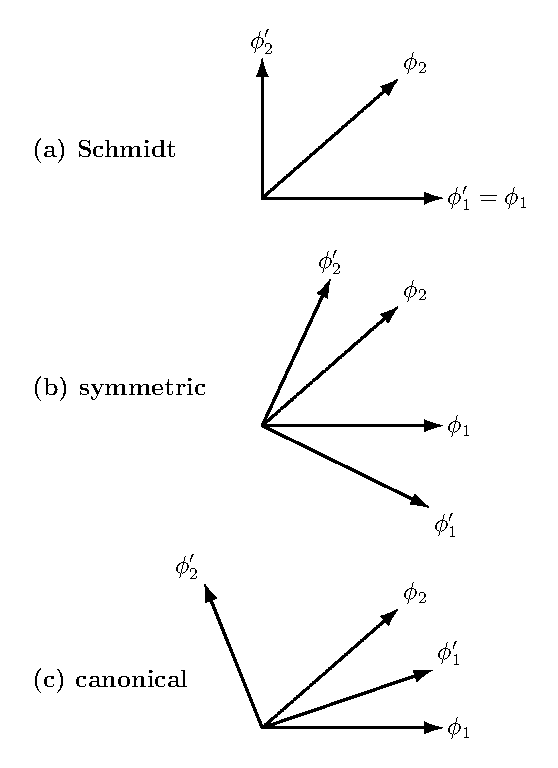
\includegraphics[width=0.42\textwidth]{ortho}
  \caption{Orthogonalization of the atomic-orbital basis.}
  \label{fig:ao-orthogonalization}
\end{figure}

\paragraph{Initial guesses for the molecular orbitals or density matrix.}

Because the Fock matrix cannot be built before a density is available, every
SCF calculation requires an initial approximation. The quality of this guess
does not change the equations being solved, but it can strongly influence the
number of iterations and, when several stationary solutions exist, the
solution to which the procedure converges.

Several initial density matrices are possible.
\begin{enumerate}
  \item Set \red{$\bP=\bO$, so that $\bF=\bH$}. This \red{core guess} is
    usually poor, but it is easy to implement.
  \item Use \red{extended H\"uckel theory or a semi-empirical method}. This
    option is inexpensive, although it is now less common.
  \item Use \red{tabulated atomic densities}. This gives the
    superposition-of-atomic-densities (SAD) guess.
  \item \red{Read the molecular orbitals from a previous calculation}. This
    option is very common and very useful.
\end{enumerate}

\paragraph{SCF convergence.}

Small changes in the energy alone do not necessarily imply that the orbitals
are self-consistent. It is therefore common to monitor both energetic changes
and a matrix residual that tests whether the occupied space is stationary
with respect to the current Fock operator.

The SCF procedure defines the iterative map
\begin{equation}
  \boxed{
    \bP^{(n)}
    \longrightarrow\bF[\bP^{(n)}]
    \longrightarrow\bP^{(n+1)}
  }.
\end{equation}
At convergence,
\begin{equation}
  \bP^{(n+1)}=\bP^{(n)}=\bP^\star.
\end{equation}
One may check the \red{energy and/or the density matrix}. At
self-consistency, the \red{generalized commutator} vanishes:
\begin{equation}
  \boxed{
    \be^{(n)}
    =\bF^{(n)}\cdot\bP^{(n)}\cdot\bS
    -\bS\cdot\bP^{(n)}\cdot\bF^{(n)}
  }.
\end{equation}
Accordingly,
\begin{equation}
  \bP^{(n)}=\bP^\star
  \qquad\Longrightarrow\qquad
  \be^{(n)}=\bO
  \qquad\Longrightarrow\qquad
  \max\abs*{\be^{(n)}}<\tau_\text{SCF}.
\end{equation}
Finally, \red{DIIS (direct inversion in the iterative subspace)} is usually
used to accelerate convergence. It extrapolates the Fock matrix from the
$m$ previous iterations according to
\begin{equation}
  \boxed{
    \bF^{(n+1)}=\sum_{i=n-m}^{n}c_i\bF^{(i)}
  }.
\end{equation}

The ordinary SCF iteration should therefore be understood as the underlying
fixed-point map. Damping, level shifting, and DIIS modify how successive
approximations are generated, but convergence is always judged against the
same self-consistency conditions.

\subsection{Direct inversion in the iterative subspace (DIIS)}

Near a self-consistent solution, several recent Fock matrices and their error
vectors contain information about the direction in which the residual is
decreasing. DIIS uses this information to form an extrapolated Fock matrix
whose estimated residual is as small as possible within the affine space
spanned by the stored iterations.

Using the $m$ stored iterations, DIIS constructs an extrapolated Fock matrix
and approximates its error vector as
\begin{align}
  \bF_\text{DIIS}^{(m+1)}
  &=\sum_{i=1}^{m}c_i\bF^{(i)},
  &
  \be_\text{DIIS}^{(m+1)}
  &\red{\approx}\sum_{i=1}^{m}c_i\be^{(i)}.
\end{align}
The coefficients minimize the squared Frobenius norm of the residual subject
to the affine constraint
\begin{equation}
  \boxed{
    \min_{\bc}
    \norm{\sum_{i=1}^{m}c_i\be^{(i)}}_F^2
    \qquad\text{subject to}\qquad
    \sum_{i=1}^{m}c_i=1
  }.
\end{equation}
Define the DIIS overlap matrix by
\begin{equation}
  B_{ij}
  =\braket*{\be^{(i)}}{\be^{(j)}}
  =\Tr\qty[\be^{(i)\dagger}\cdot\be^{(j)}].
\end{equation}
The elements of $\bB$ are therefore pairwise inner products between residual
matrices. If two iterations have very similar errors, the corresponding rows
of $\bB$ become nearly linearly dependent; this observation explains the
possible numerical singularity discussed below.
The squared residual norm is then
\begin{equation}
  \norm{\be_\text{DIIS}^{(m+1)}}_F^2
  =\sum_{ij}c_iB_{ij}c_j
  =\bc^\mathsf{T}\cdot\bB\cdot\bc.
\end{equation}

\paragraph{DIIS weights and extrapolated Fock matrix.}

The constrained minimization is described by the DIIS Lagrangian
\begin{equation}
  \mathcal{L}(\bc,\lambda)
  =\bc^\mathsf{T}\cdot\bB\cdot\bc
  -2\lambda\qty(\sum_{i=1}^{m}c_i-1).
\end{equation}
Its stationarity conditions are
\begin{equation}
  \pdv{\mathcal{L}(\bc,\lambda)}{\bc}=\bO,
  \qquad
  \pdv{\mathcal{L}(\bc,\lambda)}{\lambda}=0,
\end{equation}
which imply
\begin{equation}
  \bB\cdot\bc-\lambda\boldsymbol{1}=\bO,
  \qquad
  \sum_{i=1}^{m}c_i=1.
\end{equation}
These equations form the augmented DIIS linear system
\begin{equation}
  \begin{pmatrix}
    B_{11}&\cdots&B_{1m}&-1\\
    \vdots&\ddots&\vdots&\vdots\\
    B_{m1}&\cdots&B_{mm}&-1\\
    -1&\cdots&-1&0
  \end{pmatrix}
  \cdot
  \begin{pmatrix}
    c_1\\ \vdots\\ c_m\\ \lambda
  \end{pmatrix}
  =
  \begin{pmatrix}
    0\\ \vdots\\ 0\\ -1
  \end{pmatrix}.
\end{equation}
After solving for the coefficients, the extrapolated Fock matrix is
\begin{equation}
  \boxed{
    \bF_\text{DIIS}^{(m+1)}
    =\sum_{i=1}^{m}c_i\bF^{(i)}
  }.
\end{equation}
The linear system has dimension only \red{$(m+1)\times(m+1)$}.

The normalization constraint $\sum_i c_i=1$ makes the extrapolation affine
rather than arbitrary. In particular, if all stored Fock matrices were equal,
their extrapolated combination would reproduce that same matrix. The
Lagrange multiplier is the algebraic device that enforces this constraint.

\paragraph{DIIS algorithm.}

The complete algorithm is as follows.
\begin{enumerate}
  \item Start from the current density $\bP^{(n)}$.
  \item Build the corresponding Fock matrix
    $\bF^{(n)}=\bF[\bP^{(n)}]$.
  \item Evaluate the commutator residual
    \begin{equation}
      \be^{(n)}
      =\bF^{(n)}\cdot\bP^{(n)}\cdot\bS
      -\bS\cdot\bP^{(n)}\cdot\bF^{(n)}.
    \end{equation}
  \item Store the pair $\{\bF^{(n)},\be^{(n)}\}$ and update the DIIS
    subspace.
  \item Construct $\bB$, solve the augmented linear system, and obtain the
    coefficients $\{c_i\}$.
  \item Extrapolate the Fock matrix,
    \begin{equation}
      \bF^\text{DIIS}=\sum_i c_i\bF^{(i)}.
    \end{equation}
  \item Solve
    \begin{equation}
      \bF^\text{DIIS}\cdot\bC
      =\bS\cdot\bC\cdot\bE
    \end{equation}
    and form the next density $\bP^{(n+1)}$.
\end{enumerate}

\begin{center}
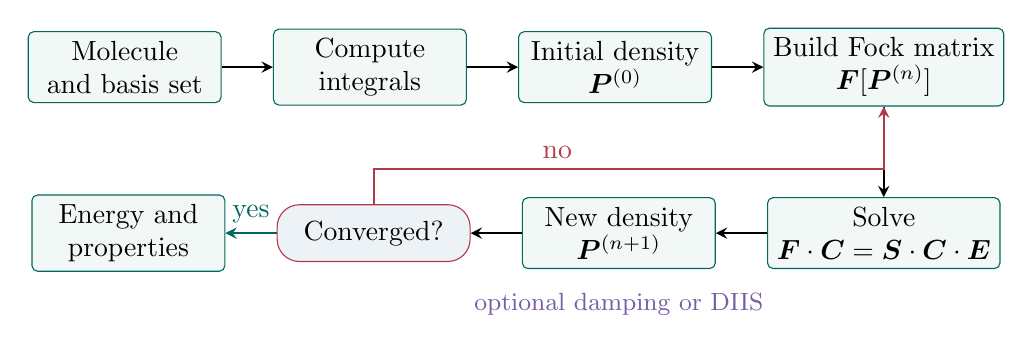
\begin{tikzpicture}[
  >=stealth,
  node distance=0.55cm and 0.65cm,
  scfstep/.style={
    draw=hfGreen,
    rounded corners=2pt,
    fill=hfGreenLight,
    minimum width=2.45cm,
    minimum height=0.72cm,
    align=center
  },
  decision/.style={
    draw=hfRed,
    rounded corners=8pt,
    fill=hfPale,
    minimum width=2.45cm,
    minimum height=0.72cm,
    align=center
  }
]
  \node[scfstep] (mol) {Molecule\\and basis set};
  \node[scfstep,right=of mol] (ints) {Compute\\integrals};
  \node[scfstep,right=of ints] (guess) {Initial density\\$\bP^{(0)}$};
  \node[scfstep,right=of guess] (fock)
    {Build Fock matrix\\$\bF[\bP^{(n)}]$};

  \node[scfstep,below=1.15cm of fock] (solve)
    {Solve\\$\bF\cdot\bC=\bS\cdot\bC\cdot\bE$};
  \node[scfstep,left=of solve] (density)
    {New density\\$\bP^{(n+1)}$};
  \node[decision,left=of density] (conv) {Converged?};
  \node[scfstep,left=of conv] (properties) {Energy and\\properties};

  \draw[->,thick] (mol)--(ints);
  \draw[->,thick] (ints)--(guess);
  \draw[->,thick] (guess)--(fock);
  \draw[->,thick] (fock)--(solve);
  \draw[->,thick] (solve)--(density);
  \draw[->,thick] (density)--(conv);
  \draw[->,thick,draw=hfGreen]
    (conv)--(properties)
    node[midway,above,text=hfGreen] {yes};
  \draw[->,thick,draw=hfRed]
    (conv.north)--++(0,0.45)-|(fock.south)
    node[pos=0.18,above,text=hfRed] {no};
  \node[below=0.18cm of density,text=hfViolet]
    {\small optional damping or DIIS};
\end{tikzpicture}
\end{center}

\paragraph{DIIS take-home messages.}

\begin{center}
  \fbox{\textbf{Key idea:} DIIS accelerates SCF convergence by finding a
  linear combination of Fock matrices.}
\end{center}
The practical consequences are
\begin{itemize}
  \item[\cmark] A small \red{rolling subspace} is normally sufficient,
    commonly $m\approx6$--$10$.
  \item[\xmark] DIIS requires additional \red{storage}, approximately
    $2mK^2$.
  \item[\xmark] The extrapolated energy is not guaranteed to decrease
    monotonically.
  \item[\xmark] $\bB$ can be \red{singular} because of nearly linear
    dependence among the residuals; a restart may be required.
  \item[\cmark] DIIS can be used for many other methods.
\end{itemize}

DIIS changes neither the Hartree--Fock energy functional nor the final
self-consistency condition. It is an acceleration strategy for reaching a
stationary solution of the same equations. This distinction matters because
rapid convergence does not by itself establish that the stationary solution
is the global Hartree--Fock minimum.

\subsection{Excited-state SCF and the maximum-overlap method}

The nonlinear character of the Hartree--Fock equations permits multiple
stationary determinants. Some correspond to non-Aufbau occupations and can be
used as state-specific approximations to electronically excited states. The
challenge is not writing such an occupation initially, but preventing the SCF
iterations from replacing it by a lower-energy Aufbau occupation.

\paragraph{Variational collapse.}

An excited determinant can be generated by promoting one or more electrons,
but the usual Aufbau occupation does not preserve that configuration.

\begin{center}
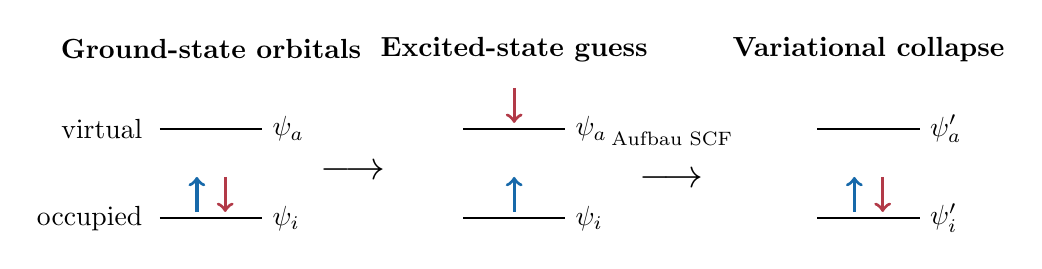
\begin{tikzpicture}[x=1cm,y=0.78cm]
  \node[font=\bfseries] at (-4.6,2.75) {Ground-state orbitals};
  \draw[thick] (-5.25,0)--(-3.95,0) node[right] {$\psi_i$};
  \draw[thick] (-5.25,1.45)--(-3.95,1.45) node[right] {$\psi_a$};
  \draw[hfBlue,very thick,->] (-4.78,0.10)--(-4.78,0.67);
  \draw[hfRed,very thick,->] (-4.42,0.67)--(-4.42,0.10);
  \node[left] at (-5.35,0) {occupied};
  \node[left] at (-5.35,1.45) {virtual};

  \node at (-2.8,0.75) {\Large$\longrightarrow$};

  \node[font=\bfseries] at (-0.75,2.75) {Excited-state guess};
  \draw[thick] (-1.40,0)--(-0.10,0) node[right] {$\psi_i$};
  \draw[thick] (-1.40,1.45)--(-0.10,1.45) node[right] {$\psi_a$};
  \draw[hfBlue,very thick,->] (-0.75,0.10)--(-0.75,0.67);
  \draw[hfRed,very thick,->] (-0.75,2.12)--(-0.75,1.55);

  \node[align=center] at (1.25,0.95) {\scriptsize Aufbau SCF\\[1mm]
    \Large$\longrightarrow$};

  \node[font=\bfseries] at (3.75,2.75) {Variational collapse};
  \draw[thick] (3.10,0)--(4.40,0) node[right] {$\psi_i'$};
  \draw[thick] (3.10,1.45)--(4.40,1.45) node[right] {$\psi_a'$};
  \draw[hfBlue,very thick,->] (3.57,0.10)--(3.57,0.67);
  \draw[hfRed,very thick,->] (3.93,0.67)--(3.93,0.10);
\end{tikzpicture}
\end{center}

After each diagonalization, Aufbau occupies the \red{lowest-energy} orbitals.
Consequently, \red{the SCF procedure tends to return to a lower-energy
solution}.

This behavior is called \red{variational collapse}. The variational principle
is not being violated: an unconstrained minimization is doing precisely what
it is designed to do. To follow a chosen excited configuration, the occupation
rule must retain the character of the targeted orbitals rather than simply
selecting the lowest eigenvalues.

\paragraph{Maximum overlap method.}

Let $\bC_\text{o}^\text{ref}$ contain the coefficients of the occupied
reference spin orbitals defining the target configuration. For every new
orbital $\chi_p^\text{new}$, compute
\begin{equation}
  O_{ip}
  =\braket{\chi_i^\text{ref}}{\chi_p^\text{new}}
  =\sum_{\mu\nu}C_{\mu i}^{\text{ref}*}
    S_{\mu\nu}C_{\nu p}^\text{new},
  \qquad
  \boxed{
    w_p=\sum_{i\in\mathcal{O}_\text{ref}}\abs{O_{ip}}^2
  }.
\end{equation}
The MOM procedure is
\begin{itemize}
  \item compute $w_p$ for every new orbital;
  \item occupy the $N$ spin orbitals with the \red{largest $w_p$};
  \item in MOM, take the reference occupied space from the previous
    iteration;
  \item in \red{IMOM}, keep the reference orbitals fixed to the initial
    guess.
\end{itemize}

\begin{center}
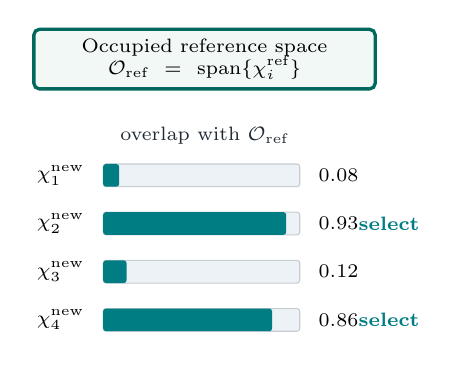
\begin{tikzpicture}[x=0.78cm,y=0.72cm,font=\scriptsize]
  \node[
    draw=hfGreen,
    very thick,
    rounded corners=2pt,
    fill=hfGreenLight,
    align=center,
    text width=4.1cm,
    minimum height=0.75cm
  ] at (2.0,5.15) {
    Occupied reference space\\
    $\mathcal{O}_\text{ref}
    =\operatorname{span}\{\chi_i^\text{ref}\}$
  };
  \node[hfInk] at (2.0,3.80) {overlap with $\mathcal{O}_\text{ref}$};

  \node[anchor=east] at (0.20,3.10) {$\chi_1^\text{new}$};
  \path[fill=hfPale,draw=hfNavy!25,rounded corners=1pt]
    (0.35,2.90) rectangle (3.55,3.30);
  \path[fill=hfTeal,rounded corners=1pt]
    (0.35,2.90) rectangle (0.61,3.30);
  \node[anchor=west] at (3.70,3.10) {$0.08$};

  \node[anchor=east] at (0.20,2.25) {$\chi_2^\text{new}$};
  \path[fill=hfPale,draw=hfNavy!25,rounded corners=1pt]
    (0.35,2.05) rectangle (3.55,2.45);
  \path[fill=hfTeal,rounded corners=1pt]
    (0.35,2.05) rectangle (3.33,2.45);
  \node[anchor=west] at (3.70,2.25) {$0.93$};
  \node[anchor=west,hfTeal,font=\scriptsize\bfseries]
    at (4.35,2.25) {select};

  \node[anchor=east] at (0.20,1.40) {$\chi_3^\text{new}$};
  \path[fill=hfPale,draw=hfNavy!25,rounded corners=1pt]
    (0.35,1.20) rectangle (3.55,1.60);
  \path[fill=hfTeal,rounded corners=1pt]
    (0.35,1.20) rectangle (0.73,1.60);
  \node[anchor=west] at (3.70,1.40) {$0.12$};

  \node[anchor=east] at (0.20,0.55) {$\chi_4^\text{new}$};
  \path[fill=hfPale,draw=hfNavy!25,rounded corners=1pt]
    (0.35,0.35) rectangle (3.55,0.75);
  \path[fill=hfTeal,rounded corners=1pt]
    (0.35,0.35) rectangle (3.10,0.75);
  \node[anchor=west] at (3.70,0.55) {$0.86$};
  \node[anchor=west,hfTeal,font=\scriptsize\bfseries]
    at (4.35,0.55) {select};
\end{tikzpicture}
\end{center}

Thus, MOM selects orbitals \red{by orbital character, not by energy}.

The weight $w_p$ measures the total squared projection of a new orbital onto
the reference occupied subspace. It is insensitive to unitary rotations within
that reference space, so the selection is based on the subspace representing
the target configuration rather than on an arbitrary labeling of individual
reference orbitals.

\paragraph{MOM-based SCF.}

The MOM-SCF cycle is
\begin{center}
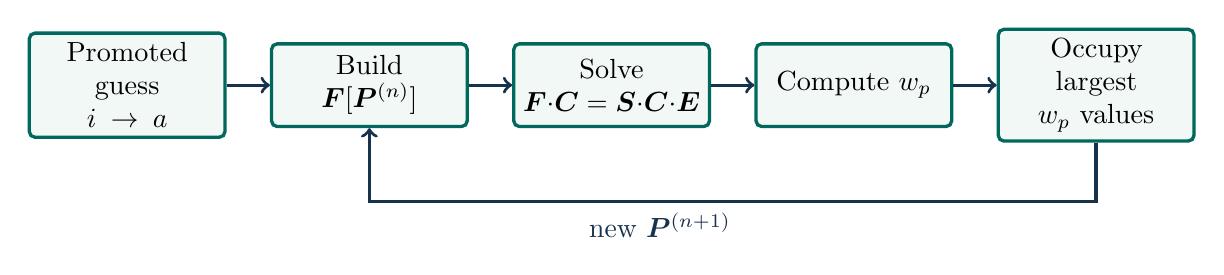
\begin{tikzpicture}[
  node distance=0.55cm and 0.55cm,
  box/.style={
    draw=hfGreen,
    very thick,
    rounded corners=2pt,
    fill=hfGreenLight,
    minimum height=1.05cm,
    text width=2.25cm,
    align=center
  },
  arrow/.style={->,very thick,hfNavy}
]
  \node[box] (guess) {Promoted guess\\$i\rightarrow a$};
  \node[box,right=of guess] (fock) {Build\\$\bF[\bP^{(n)}]$};
  \node[box,right=of fock] (solve)
    {Solve\\$\bF\cdot\bC=\bS\cdot\bC\cdot\bE$};
  \node[box,right=of solve] (overlap) {Compute $w_p$};
  \node[box,right=of overlap] (occupy) {Occupy largest\\$w_p$ values};

  \draw[arrow] (guess)--(fock);
  \draw[arrow] (fock)--(solve);
  \draw[arrow] (solve)--(overlap);
  \draw[arrow] (overlap)--(occupy);
  \draw[arrow] (occupy.south)--++(0,-0.75)-|(fock.south)
    node[pos=0.30,below] {new $\bP^{(n+1)}$};
\end{tikzpicture}
\end{center}

Conventional SCF occupies the lowest orbital energies,
\begin{equation}
  \epsilon_1\leq\epsilon_2\leq\cdots\leq\epsilon_N,
\end{equation}
and therefore finds a low-energy solution. MOM-SCF instead occupies the
largest overlap weights,
\begin{equation}
  w_1\geq w_2\geq\cdots\geq w_N,
\end{equation}
and therefore follows a chosen SCF solution. Thus, \red{MOM changes the
occupation to target non-Aufbau stationary solutions of the HF equations}.

\paragraph{What does a MOM calculation give?}

The principal gains are
\begin{itemize}
  \item[\cmark] a higher-energy stationary solution of the HF equations;
  \item[\cmark] useful excitation energies for states dominated by a single
    electronic configuration;
  \item[\cmark] full orbital relaxation for the targeted configuration;
  \item[\cmark] a state-specific density and molecular properties;
  \item[\cmark] the same formal cost per SCF iteration, although convergence
    may be more difficult.
\end{itemize}
The corresponding cautions are
\begin{itemize}
  \item[\xmark] the result is still a single determinant;
  \item[\xmark] spin symmetry may be broken;
  \item[\xmark] different SCF states are not necessarily orthogonal;
  \item[\xmark] convergence depends on the initial promoted orbitals;
  \item[\xmark] MOM can drift or converge to an unintended solution.
\end{itemize}

MOM should consequently be viewed as an occupation-following prescription,
not as a new electronic-structure approximation. It selects a particular
stationary solution of the Hartree--Fock equations and allows the orbitals of
that determinant to relax self-consistently.

\subsection{Molecular properties and orbital analysis}

Once a self-consistent density matrix has been obtained, one-electron
properties can be evaluated by contracting that density with the appropriate
property integrals. The same density also provides the starting point for
population analyses. Individual canonical orbitals, however, are not unique
within the occupied and virtual subspaces, which motivates localized-orbital
representations.

\paragraph{Dipole moments.}

The dipole moment illustrates the general structure of a one-electron
property: a quantum-mechanical electronic expectation value is combined with
the corresponding classical nuclear contribution.

The classical dipole vector is
\begin{equation}
  \boldsymbol{\mu}=(\mu_x,\mu_y,\mu_z)
  =\underbrace{\green{\sum_i q_i\br_i}}
    _{\text{\green{classical definition}}}.
\end{equation}
For a molecule, the corresponding quantum-mechanical expression separates
the electronic and nuclear contributions:
\begin{align}
  \boldsymbol{\mu}
  &=(\mu_x,\mu_y,\mu_z)
  \\
  &=\underbrace{\red{\mel{\Psi_0}{-\sum_{i=1}^{N}\br_i}{\Psi_0}}}
      _{\text{\red{electrons}}}
    +\underbrace{\blue{\sum_{A=1}^{M}Z_A\bR_A}}
      _{\text{\blue{nuclei}}}
  \\
  &=\red{-\sum_{\mu\nu}P_{\mu\nu}\rmel{\nu}{\br}{\mu}}
    +\blue{\sum_{A=1}^{M}Z_A\bR_A}.
\end{align}
For example, its $x$ component is
\begin{equation}
  \mu_x
  =\red{-\sum_{\mu\nu}P_{\mu\nu}\rmel{\nu}{x}{\mu}}
  +\blue{\sum_{A=1}^{M}Z_AX_A},
  \qquad
  \underbrace{\rmel{\nu}{x}{\mu}}_{\text{one-electron integrals}}
  =\int\phi_\nu^*(\br)\,x\,\phi_\mu(\br)\dd{\br}.
\end{equation}

\paragraph{Charge analysis.}

An atomic charge is not itself a direct observable of the molecular
wavefunction. Population analyses define such charges by adopting a rule for
partitioning the density among atom-centered basis functions. Mulliken and
L\"owdin analyses differ precisely in this partitioning convention.

The electron density is
\begin{equation}
  \rho(\br)=\sum_{\mu\nu}\phi_\mu(\br)P_{\mu\nu}\phi_\nu^*(\br),
  \qquad
  \int\rho(\br)\dd{\br}=N.
\end{equation}
Consequently,
\begin{equation}
  N=\sum_{\mu\nu}P_{\mu\nu}S_{\nu\mu}
  =\sum_\mu(\bP\cdot\bS)_{\mu\mu}
  =\Tr(\bP\cdot\bS).
\end{equation}
Assuming that the basis functions are atom-centered, the Mulliken population
analysis assigns the net charge
\begin{equation}
  \underbrace{\blue{q_A^\text{Mulliken}}}_{\text{net charge on $A$}}
  =Z_A-\sum_{\mu\in A}(\bP\cdot\bS)_{\mu\mu}.
\end{equation}
For L\"owdin population analysis, cyclic invariance of the trace,
$\Tr(\bA\cdot\bB)=\Tr(\bB\cdot\bA)$, gives, for any $\alpha$,
\begin{equation}
  N=\sum_\mu
  (\bS^\alpha\cdot\bP\cdot\bS^{1-\alpha})_{\mu\mu}.
\end{equation}
For \red{$\alpha=1/2$}, this becomes
\begin{equation}
  N=\sum_\mu
  (\bS^{1/2}\cdot\bP\cdot\bS^{1/2})_{\mu\mu},
  \qquad\Rightarrow\qquad
  \red{q_A^\text{L\"owdin}}
  =Z_A-\sum_{\mu\in A}
  (\bS^{1/2}\cdot\bP\cdot\bS^{1/2})_{\mu\mu}.
\end{equation}

\paragraph{Localized orbitals.}

Canonical orbitals diagonalize the occupied-occupied and virtual-virtual
blocks of the Fock matrix, but they are often delocalized over an entire
molecule. Because unitary rotations within either subspace leave the Slater
determinant invariant, the same Hartree--Fock state can be represented by
orbitals chosen to satisfy a localization criterion.

At HF convergence and after canonicalization and localization, the Fock
matrix passes through the sequence
\begin{equation}
  \bff=
  \mqty(\bff_\text{oo}&\bff_\text{ov}\\
        \bff_\text{vo}&\bff_\text{vv})
  \xrightarrow{\text{HF convergence}}
  \mqty(\bff_\text{oo}&\bO\\
        \bO&\bff_\text{vv})
  \xrightarrow{\text{canonicalization}}
  \mqty(\bepsilon_\text{o}&\bO\\
        \bO&\bepsilon_\text{v})
  \xrightarrow{\text{localization}}
  \mqty(\widetilde{\bff}_\text{oo}&\bO\\
        \bO&\widetilde{\bff}_\text{vv}).
\end{equation}
The localized occupied orbitals are obtained through a unitary
transformation,
\begin{equation}
  \boxed{
    \widetilde{\bC}_\text{o}
    =\bC_\text{o}\cdot\purple{\bU},
    \qquad
    \purple{\bU}^\dagger\cdot\purple{\bU}=\bI
    \quad\Longleftrightarrow\quad
    \text{\purple{unitary transformation}}
  }.
\end{equation}
For a closed-shell determinant, the density matrix is unchanged:
\begin{equation}
  \widetilde{\bP}
  =2\widetilde{\bC}_\text{o}
   \cdot\widetilde{\bC}_\text{o}^\dagger
  =2\bC_\text{o}\cdot\bC_\text{o}^\dagger
  =\bP.
\end{equation}
The determinant changes only by a phase,
\begin{equation}
  \ket*{\widetilde{\Psi}_0}
  =\det(\purple{\bU})\ket{\Psi_0},
\end{equation}
so the \red{density}, \red{energy}, and \red{every expectation value} are
unchanged.

\begin{center}
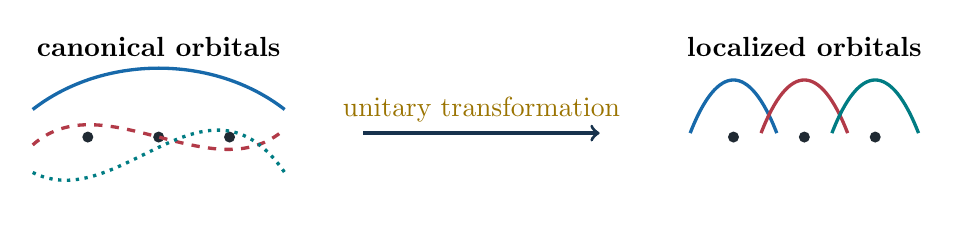
\begin{tikzpicture}[x=1cm,y=1cm]
  \node[font=\bfseries] at (-4.1,1.15) {canonical orbitals};
  \node[font=\bfseries] at (4.1,1.15) {localized orbitals};
  \foreach \x in {-5.0,-4.1,-3.2}{\fill[hfInk] (\x,0) circle (0.07);}
  \draw[hfBlue,very thick]
    (-5.7,0.35)..controls(-4.8,1.05)and(-3.4,1.05)..(-2.5,0.35);
  \draw[hfRed,very thick,dashed]
    (-5.7,-0.10)..controls(-4.8,0.70)and(-3.4,-0.70)..(-2.5,0.10);
  \draw[hfTeal,very thick,dotted]
    (-5.7,-0.45)..controls(-4.6,-1.00)and(-3.5,1.00)..(-2.5,-0.45);
  \draw[hfNavy,very thick,->] (-1.5,0.05)--(1.5,0.05)
    node[midway,above] {\purple{unitary transformation}};
  \foreach \x in {3.2,4.1,5.0}{\fill[hfInk] (\x,0) circle (0.07);}
  \draw[hfBlue,very thick]
    (2.65,0.05)..controls(3.0,0.95)and(3.4,0.95)..(3.75,0.05);
  \draw[hfRed,very thick]
    (3.55,0.05)..controls(3.9,0.95)and(4.3,0.95)..(4.65,0.05);
  \draw[hfTeal,very thick]
    (4.45,0.05)..controls(4.8,0.95)and(5.2,0.95)..(5.55,0.05);
\end{tikzpicture}
\end{center}

Only \red{occupied-occupied} or \red{virtual-virtual} rotations are
invariant. Mixing \red{occupied and virtual} orbitals changes the wavefunction
and the energy. Localization functionals are generally \red{nonconvex}, so
different guesses may converge to different local extrema.

This invariance separates two logically distinct operations. Orbital
optimization mixes occupied and virtual spaces and changes the physical
determinant; localization rotates only within an already optimized subspace
and changes its representation without changing the state.

\paragraph{Localization procedures.}

The Edmiston--Ruedenberg functional is
\begin{equation}
  \boxed{
    \Omega_\text{ER}
    =\sum_i\rbraket{\psi_i\psi_i}{\psi_i\psi_i}
    \quad\longrightarrow\quad
    \max\ \text{orbital self-repulsion}
  }.
\end{equation}
The Foster--Boys functional may be written in two equivalent forms:
\begin{align}
  \Omega_\text{BF}
  &=\frac{1}{2}\sum_i
    \qty[\mel{\psi_i\psi_i}{r_{12}^2}{\psi_i\psi_i}]
    \quad\longrightarrow\quad
    \min\ \text{spatial extent}
  \\
  &\red{\equiv}\sum_i\qty[
    \mel{\psi_i}{r^2}{\psi_i}
    -\abs{\mel{\psi_i}{\br}{\psi_i}}^2]
    \quad\longrightarrow\quad
    \max\ \text{distance between centroids}.
\end{align}
Its strengths are
\begin{itemize}
  \item[\cmark] it requires only one-electron integrals;
  \item[\cmark] it produces compact bonds and lone pairs.
\end{itemize}
Its limitations are
\begin{itemize}
  \item[\xmark] it does not explicitly preserve $\sigma/\pi$ separation;
  \item[\xmark] diffuse virtual orbitals may be difficult to localize.
\end{itemize}

For an atomic population $q_i^A$ of orbital $i$ on atom $A$, the original
Pipek--Mezey criterion maximizes
\begin{equation}
  \boxed{
    \Omega_\text{PM}=\sum_A\sum_i\abs*{q_i^A}^2
  },
\end{equation}
using the Mulliken populations
\begin{equation}
  q_i^A
  =\sum_{\mu\in A}\sum_\nu
    C_{\mu i}^*S_{\mu\nu}C_{\nu i}.
\end{equation}
Its strengths are
\begin{itemize}
  \item[\cmark] it often preserves separation between $\sigma$ and $\pi$
    orbitals;
  \item[\cmark] it produces intuitive bonds, lone pairs, and core orbitals.
\end{itemize}
Its limitations are
\begin{itemize}
  \item[\xmark] the original Mulliken form can be basis-set dependent;
  \item[\xmark] L\"owdin populations or intrinsic atomic orbitals provide
    more robust alternatives.
\end{itemize}
There is \red{no universally best localized-orbital set}; the criterion should
match the intended interpretation or computational use.

\paragraph{Summary of orbital localization.}

The following quantities remain unchanged:
\begin{itemize}
  \item the occupied subspace and Slater determinant;
  \item the density matrix and electron density;
  \item the HF energy and molecular properties;
  \item the zero occupied-virtual Fock block,
    \begin{equation}
      \widetilde{\bff}_\text{ov}=\bff_\text{ov}=\bO.
    \end{equation}
\end{itemize}
What changes is that localized orbitals are generally not eigenfunctions of
the Fock operator:
\begin{equation}
  \widetilde{\bff}_\text{oo}
  =\purple{\bU}^\dagger\cdot\bepsilon_\text{o}\cdot\purple{\bU}.
\end{equation}
Orbital energies therefore cannot be assigned to localized orbitals.

Localization is useful to
\begin{itemize}
  \item identify bonds, lone pairs, and fragments;
  \item enable local correlation and embedding methods;
  \item select active spaces and domains;
  \item construct Wannier functions in periodic systems.
\end{itemize}
The practical cautions are to
\begin{itemize}
  \item localize occupied and virtual spaces separately;
  \item often localize core and valence orbitals separately;
  \item check for multiple extrema and discontinuous solutions;
  \item remember that spatial symmetry may be lost.
\end{itemize}

\section{Open-shell and generalized Hartree--Fock methods}

The restricted closed-shell ansatz is efficient and preserves spin symmetry,
but it is too restrictive whenever the two spin populations require different
spatial descriptions. Open-shell species and bond-breaking problems therefore
motivate a hierarchy of increasingly flexible single-determinant
wavefunctions. Unrestricted Hartree--Fock relaxes the requirement that
$\alpha$ and $\beta$ electrons share spatial orbitals, while generalized
Hartree--Fock also removes the requirement that each orbital possess a fixed
spin projection.

\subsection{Unrestricted Hartree--Fock theory}
\subsubsection{The unrestricted ansatz}

In restricted Hartree--Fock, a doubly occupied spatial orbital is shared by
one $\alpha$ and one $\beta$ electron. Unrestricted Hartree--Fock removes this
pairing constraint. For open-shell systems, one uses \red{unrestricted spin
orbitals},
\begin{equation}
  \chi_p^\text{UHF}(\bx)
  =\begin{cases}
    \alpha(\omega)\blue{\psi_p^\alpha(\br)},\\
    \beta(\omega)\red{\psi_p^\beta(\br)}.
  \end{cases}
\end{equation}
The $\alpha$ and $\beta$ spatial orbitals are therefore allowed to differ.
The consequences stated in the slides are
\begin{itemize}
  \item UHF may break spin symmetry: the determinant need not be an
    eigenfunction of $\purple{\chS^2}$;
  \item the HF wavefunction is no longer a pure spin function;
  \item singlets may be contaminated by triplets, quintets, and higher-spin
    states;
  \item doublets may be contaminated by quartets, sextets, and higher-spin
    states.
\end{itemize}
Generalized Hartree--Fock also permits spin mixing and need not preserve
$\violet{\chS_z}$. Its orbitals have the form
\begin{equation}
  \chi_p^\text{GHF}(\bx)
  =\alpha(\omega)\blue{\psi_p^\alpha(\br)}
  +\beta(\omega)\red{\psi_p^\beta(\br)}
  \qquad\Rightarrow\qquad
  \red{\text{two-component spinor}}.
\end{equation}

The additional variational freedom can lower the energy, but it changes the
symmetry content of the determinant. In particular, the distinction between a
useful broken-symmetry energy and a spin-pure wavefunction must be kept in mind
throughout the following discussion.

\subsubsection{The unrestricted Hartree--Fock equations and energy}

The UHF determinant contains two independently optimized orthonormal orbital
sets. Variation with respect to these two sets gives two coupled orbital
equations. To \red{minimize the UHF energy}, the unrestricted spatial orbitals must be
eigenfunctions of the separate \red{$\alpha$ and $\beta$ Fock operators}:
\begin{align}
  &\boxed{
    \blue{f^\alpha(\br_1)\psi_i^\alpha(\br_1)
    =\epsilon_i^\alpha\psi_i^\alpha(\br_1)}
  },
  &
  &\boxed{
    \red{f^\beta(\br_1)\psi_i^\beta(\br_1)
    =\epsilon_i^\beta\psi_i^\beta(\br_1)}
  }.
\end{align}
The two Fock operators are
\begin{align}
  \blue{f^\alpha(\br_1)}
  &=h(\br_1)
    +\sum_i^{N^\alpha}
      \qty[\blue{J_i^\alpha(\br_1)-K_i^\alpha(\br_1)}]
    +\sum_i^{N^\beta}\red{J_i^\beta(\br_1)},
  \\
  \red{f^\beta(\br_1)}
  &=h(\br_1)
    +\sum_i^{N^\beta}
      \qty[\red{J_i^\beta(\br_1)-K_i^\beta(\br_1)}]
    +\sum_i^{N^\alpha}\blue{J_i^\alpha(\br_1)}.
\end{align}
The \blue{Coulomb} and \violet{exchange} operators are defined by
\begin{align}
  \blue{J_i^\sigma(\br_1)}
  &=\int\psi_i^{\sigma *}(\br_2)r_{12}^{-1}
    \psi_i^\sigma(\br_2)\dd{\br_2},
  \\
  \violet{K_i^\sigma(\br_1)}\psi_j^\sigma(\br_1)
  &=\qty[\int\psi_i^{\sigma *}(\br_2)r_{12}^{-1}
    \psi_j^\sigma(\br_2)\dd{\br_2}]
    \psi_i^\sigma(\br_1).
\end{align}

Each spin population contributes a Coulomb field felt by electrons of either
spin. Exchange, however, acts only between electrons carrying the same spin
function because opposite spin functions are orthogonal. Consequently, the
two Fock operators differ whenever the $\alpha$ and $\beta$ densities differ,
yet they remain coupled through their mutual Coulomb contributions.

\paragraph{The UHF energy.}

The UHF energy comprises three contributions:
\begin{equation}
  E_\text{UHF}
  =\blue{E_\text{UHF}^{\alpha\alpha}}
  +\red{E_\text{UHF}^{\beta\beta}}
  +\violet{E_\text{UHF}^{\alpha\beta}}.
\end{equation}
Explicitly,
\begin{equation}
\boxed{
\begin{aligned}
  E_\text{UHF}
  ={}&\blue{\sum_i^{N^\alpha}h_{ii}^\alpha
    +\frac{1}{2}\sum_{ij}^{N^\alpha}
      \qty(J_{ij}^{\alpha\alpha}-K_{ij}^{\alpha\alpha})}
  \\
  &+\red{\sum_i^{N^\beta}h_{ii}^\beta
    +\frac{1}{2}\sum_{ij}^{N^\beta}
      \qty(J_{ij}^{\beta\beta}-K_{ij}^{\beta\beta})}
  \\
  &+\violet{\sum_i^{N^\alpha}\sum_j^{N^\beta}
    J_{ij}^{\alpha\beta}}.
\end{aligned}
}
\end{equation}
The matrix elements are
\begin{align}
  h_{ii}^\sigma
  &=\mel{\psi_i^\sigma}{h}{\psi_i^\sigma},
  &
  J_{ij}^{\sigma\sigma'}
  &=\braket*{\psi_i^\sigma\psi_j^{\sigma'}}
    {\psi_i^\sigma\psi_j^{\sigma'}},
  &
  K_{ij}^{\sigma\sigma}
  &=\braket*{\psi_i^\sigma\psi_j^\sigma}
    {\psi_j^\sigma\psi_i^\sigma}.
\end{align}
There is \red{no exchange between opposite-spin electrons}.

The factors of one half in the same-spin contributions remove double counting
of electron pairs. The opposite-spin Coulomb term is written only once as a
double sum over the two populations and therefore requires no such factor.

\paragraph{Problem: UHF energy of the \ce{Li} atom.}

\violet{\textit{``Write down the UHF energy of the doublet state of the
lithium atom.''}}

\begin{center}
\begin{tikzpicture}[>=stealth]
  \draw[thick] (-1.4,2.2)--(-0.4,2.2);
  \draw[thick] (0.4,2.2)--(1.4,2.2);
  \node[left] at (-1.4,2.2) {$2s^\alpha$};
  \node[right] at (1.4,2.2) {$2s^\beta$};

  \draw[thick] (-1.4,0.3)--(-0.4,0.3);
  \draw[thick] (0.4,0.3)--(1.4,0.3);
  \node[left] at (-1.4,0.3) {$1s^\alpha$};
  \node[right] at (1.4,0.3) {$1s^\beta$};

  \draw[->,very thick,blue] (-0.9,1.85)--(-0.9,2.45);
  \draw[->,very thick,blue] (-0.9,-0.05)--(-0.9,0.55);
  \draw[->,very thick,red] (0.9,0.65)--(0.9,0.05);
  \node[blue] at (-0.9,-0.75) {$\alpha$};
  \node[red] at (0.9,-0.75) {$\beta$};
\end{tikzpicture}
\end{center}

\paragraph{Solution.}

For the occupation shown above,
\begin{equation}
  E_\text{UHF}
  =h_{11}^\alpha+h_{11}^\beta+h_{22}^\alpha
  +J_{12}^{\alpha\alpha}-K_{12}^{\alpha\alpha}
  +J_{11}^{\alpha\beta}+J_{21}^{\alpha\beta}.
\end{equation}

The same-spin interaction between the $1s^\alpha$ and $2s^\alpha$ electrons
contains both Coulomb and exchange contributions. The two interactions with
the $1s^\beta$ electron are purely Coulombic, exactly as required by the spin
selection rule above.

\subsubsection{The Pople--Nesbet matrix equations}

The continuous UHF equations are reduced to matrix form in the same way as
the restricted equations, except that a separate coefficient matrix and Fock
matrix are required for each spin. The unrestricted spatial orbitals are
expanded in the same AO basis with
separate spin-dependent coefficients:
\begin{align}
  \psi_i^\alpha(\br)
  &=\sum_{\mu=1}^{K}\blue{C_{\mu i}^\alpha}\phi_\mu(\br),
  &
  \psi_i^\beta(\br)
  &=\sum_{\mu=1}^{K}\red{C_{\mu i}^\beta}\phi_\mu(\br).
\end{align}
The resulting Pople--Nesbet equations are
\begin{align}
  \blue{\bF^\alpha}\cdot\blue{\bC^\alpha}
  &=\bS\cdot\blue{\bC^\alpha}\cdot\bE^\alpha,
  &
  \red{\bF^\beta}\cdot\red{\bC^\beta}
  &=\bS\cdot\red{\bC^\beta}\cdot\bE^\beta.
\end{align}
Their spin-dependent Fock matrices are
\begin{align}
  \blue{F_{\mu\nu}^\alpha}
  ={}&H_{\mu\nu}
  +\sum_{\lambda\sigma}\blue{P_{\lambda\sigma}^\alpha}
    \qty[
      \rbraket{\mu\nu}{\sigma\lambda}
      -\rbraket{\mu\lambda}{\sigma\nu}
    ]
  \notag\\
  &+\sum_{\lambda\sigma}\red{P_{\lambda\sigma}^\beta}
    \rbraket{\mu\nu}{\sigma\lambda},
  \\
  \red{F_{\mu\nu}^\beta}
  ={}&H_{\mu\nu}
  +\sum_{\lambda\sigma}\red{P_{\lambda\sigma}^\beta}
    \qty[
      \rbraket{\mu\nu}{\sigma\lambda}
      -\rbraket{\mu\lambda}{\sigma\nu}
    ]
  \notag\\
  &+\sum_{\lambda\sigma}\blue{P_{\lambda\sigma}^\alpha}
    \rbraket{\mu\nu}{\sigma\lambda}.
\end{align}
Both $\blue{\bF^\alpha}$ and $\red{\bF^\beta}$ depend on
$\blue{\bC^\alpha}$ and $\red{\bC^\beta}$. Therefore, \red{the $\alpha$
and $\beta$ orbitals are coupled}.

Thus the two generalized eigenvalue problems cannot be solved independently.
Updating either spin density changes the Coulomb potential in both Fock
matrices and changes the exchange potential in the Fock matrix of the same
spin.

\paragraph{Unrestricted density matrices.}

The spin-up and spin-down density matrices are
\begin{align}
  &\boxed{
    \blue{P_{\mu\nu}^\alpha}
    =\sum_{i=1}^{N^\alpha}C_{\mu i}^\alpha C_{\nu i}^{\alpha *}
    \quad\Longleftrightarrow\quad\blue{\bP^\alpha}
  },
  &
  &\boxed{
    \red{P_{\mu\nu}^\beta}
    =\sum_{i=1}^{N^\beta}C_{\mu i}^\beta C_{\nu i}^{\beta *}
    \quad\Longleftrightarrow\quad\red{\bP^\beta}
  }.
\end{align}
For $\sigma=\alpha$ or $\beta$, the corresponding real-space density and
its normalization are
\begin{align}
  \rho^\sigma(\br)
  &=\sum_{\mu\nu}\phi_\mu(\br)P_{\mu\nu}^\sigma
    \phi_\nu^*(\br),
  &
  \int\rho^\sigma(\br)\dd{\br}
  &=N^\sigma.
\end{align}
Finally, the total and spin density matrices are
\begin{align}
  \underbrace{\blue{\bP^\text{T}}}_{\blue{\text{charge density}}}
  &=\blue{\bP^\alpha}+\red{\bP^\beta},
  &
  \underbrace{\violet{\bP^\text{S}}}_{\violet{\text{spin density}}}
  &=\blue{\bP^\alpha}-\red{\bP^\beta}.
\end{align}

The sum $\bP^\text{T}$ determines the total charge density. The difference
$\bP^\text{S}$ measures the spatial imbalance between the two spin
populations and is the matrix representation of the collinear spin density.

\subsubsection{The unrestricted SCF procedure}

The practical UHF SCF algorithm mirrors the restricted procedure, but both
spin densities must be propagated until they are mutually self-consistent. It
is
\begin{enumerate}
  \item \red{Specify the molecule} $\{\bR_A\}$ and $\{Z_A\}$ and the
    \red{basis set} $\{\phi_\mu\}$, as in RHF.
  \item Calculate $S_{\mu\nu}$, $H_{\mu\nu}$, and
    $\braket{\mu\nu}{\lambda\sigma}$, as in RHF.
  \item Diagonalize $\bS$ and compute $\bX$, as in RHF.
  \item Choose \red{initial density matrices} $\bP^\alpha$ and $\bP^\beta$,
    then iterate:
    \begin{enumerate}
      \item[1a.] Calculate $\bG^\alpha$ and
        $\bF^\alpha=\bH+\bG^\alpha$.
      \item[1b.] Calculate $\bG^\beta$ and
        $\bF^\beta=\bH+\bG^\beta$.
      \item[2.] Compute
        $(\bF^\alpha)'=\bX^\dag\cdot\bF^\alpha\cdot\bX$ and
        $(\bF^\beta)'=\bX^\dag\cdot\bF^\beta\cdot\bX$.
      \item[3a.] Diagonalize $(\bF^\alpha)'$ to obtain
        $(\bC^\alpha)'$ and $\bE^\alpha$.
      \item[3b.] Diagonalize $(\bF^\beta)'$ to obtain
        $(\bC^\beta)'$ and $\bE^\beta$.
      \item[4.] Calculate
        $\bC^\alpha=\bX\cdot(\bC^\alpha)'$ and
        $\bC^\beta=\bX\cdot(\bC^\beta)'$.
      \item[5.] Form the \red{new density matrices} $\bP^\alpha$ and
        $\bP^\beta$, and compute
        $\bP^\text{T}=\bP^\alpha+\bP^\beta$.
      \item[6.] Test convergence. If the calculation is not converged,
        return to step 1a.
    \end{enumerate}
  \item Evaluate the desired observables, including $E_\text{UHF}$.
\end{enumerate}

Convergence therefore requires a fixed point of the coupled map
\begin{equation}
  (\bP^\alpha,\bP^\beta)
  \longrightarrow
  (\bF^\alpha,\bF^\beta)
  \longrightarrow
  (\bP^\alpha,\bP^\beta).
\end{equation}
Different initial spin densities can lead to different stationary solutions,
especially where restricted spin symmetry becomes unstable.

\subsection{Symmetry breaking in the dissociation of \ce{H2}}

The dissociation of the hydrogen molecule is the simplest illustration of
both the usefulness and the limitation of unrestricted Hartree--Fock. It
shows explicitly how relaxing the equality of the two spatial orbitals repairs
the restricted dissociation energy while producing a wavefunction that is no
longer a pure eigenfunction of $\chS^2$.

Start from one normalized $1s$ function on each atom:
\begin{equation}
  \boxed{
    \psi_g=\frac{\phi_A+\phi_B}{\sqrt{2(1+S)}},
    \qquad
    \psi_u=\frac{\phi_A-\phi_B}{\sqrt{2(1-S)}}
  },
  \qquad S=\braket{\phi_A}{\phi_B}.
\end{equation}
For two electrons in two spatial orbitals, UHF reduces to a
\red{single-parameter problem}.

\begin{center}
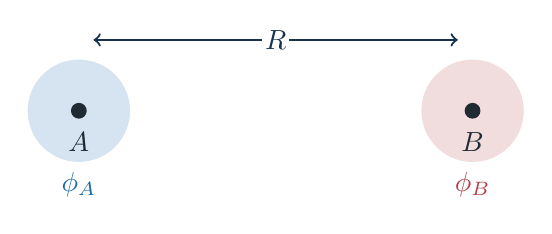
\begin{tikzpicture}[x=1.25cm,y=1.25cm]
  \fill[hfBlue!18] (-2.0,0) circle (0.52);
  \fill[hfRed!18] (2.0,0) circle (0.52);
  \fill[hfInk] (-2.0,0) circle (0.08) node[below=0.15cm] {$A$};
  \fill[hfInk] (2.0,0) circle (0.08) node[below=0.15cm] {$B$};
  \draw[hfNavy,thick,<->] (-1.85,0.72)--(1.85,0.72)
    node[midway,fill=white,inner sep=1pt] {$R$};
  \node[hfBlue] at (-2.0,-0.75) {$\phi_A$};
  \node[hfRed] at (2.0,-0.75) {$\phi_B$};
\end{tikzpicture}
\end{center}

\paragraph{The RHF problem.}

In the restricted description both electrons occupy the gerade bonding
orbital. The RHF wavefunction and energy are
\begin{equation}
  \ket{\Psi_\text{RHF}}=\ket{\psi_g\Bar{\psi}_g},
  \qquad
  E_\text{RHF}=2h_{gg}+J_{gg}+\frac{1}{R}.
\end{equation}
At large $R$, where $S\rightarrow0$,
\begin{equation}
  \psi_g(1)\psi_g(2)\longrightarrow\frac{1}{2}\qty[
    \underbrace{\phi_A(1)\phi_B(2)+\phi_B(1)\phi_A(2)}
      _{\text{covalent}}
    +\underbrace{\phi_A(1)\phi_A(2)+\phi_B(1)\phi_B(2)}
      _{\text{ionic}}
  ].
\end{equation}
RHF retains \red{$50\%$ ionic character} as $R\rightarrow\infty$. Both
electrons are forced to share the same spatial orbital, so its energy lies
above that of two separated H atoms. Hence, \red{RHF is qualitatively correct
near equilibrium but not at dissociation}.

The defect is not caused by an inadequate optimization of the bonding orbital
within RHF. It follows from the restricted ansatz itself: placing both
electrons in the same spatial orbital inevitably retains the ionic
configurations together with the covalent ones.

\paragraph{The UHF problem.}

The two-dimensional orbital space spanned by $\psi_g$ and $\psi_u$ permits
the $\alpha$ and $\beta$ orbitals to rotate in opposite directions. The UHF
orbitals can be parametrized as
\begin{equation}
  \boxed{
  \begin{aligned}
    \psi^\alpha(\theta)&=\cos\theta\,\psi_g+\sin\theta\,\psi_u,\\
    \psi^\beta(\theta)&=\cos\theta\,\psi_g-\sin\theta\,\psi_u,
  \end{aligned}}
  \qquad
  \braket{\psi^\alpha}{\psi^\beta}=\cos(2\theta).
\end{equation}
The two choices $\pm\theta$ are degenerate and exchange the spin
localization.

The parameter $\theta$ therefore provides a continuous path from the
restricted determinant at $\theta=0$ to a determinant with one spin orbital
localized on each atom at $\theta=\pi/4$. The orbital overlap
$\cos(2\theta)$ decreases along this path and vanishes at complete
localization.

\begin{center}
\begin{minipage}[t]{0.31\textwidth}
  \centering\textbf{$\theta=0^\circ$: RHF limit}

  \HtwoOrbitalPlot{0}

  $\psi^\alpha=\psi^\beta=\psi_g$
\end{minipage}\hfill
\begin{minipage}[t]{0.31\textwidth}
  \centering\textbf{$0<\theta<45^\circ$: polarization}

  \HtwoOrbitalPlot{22.5}

  $\alpha$ shifts to $A$; $\beta$ shifts to $B$
\end{minipage}\hfill
\begin{minipage}[t]{0.31\textwidth}
  \centering\textbf{$\theta=45^\circ$: dissociation}

  \HtwoOrbitalPlot{45}

  $\psi^\alpha\to\phi_A$; $\psi^\beta\to\phi_B$
\end{minipage}
\end{center}

With $J_{pq}=\rbraket{pp}{qq}$ and $K_{pq}=\rbraket{pq}{pq}$, the energy is
\begin{align}
  E_\text{UHF}(\theta)={}&2\cos^2\theta\,h_{gg}
  +2\sin^2\theta\,h_{uu}
  +\cos^4\theta\,J_{gg}
  +\sin^4\theta\,J_{uu}
  \notag\\
  &+2\sin^2\theta\cos^2\theta\qty(J_{gu}-2K_{gu}).
\end{align}
Besides the restricted stationary point $\theta=0$, a
\red{broken-symmetry stationary solution} satisfies
\begin{equation}
  \boxed{
    \cos^2\theta^\star
    =\frac{h_{uu}-h_{gg}+J_{uu}-J_{gu}+2K_{gu}}
      {J_{gg}+J_{uu}-2J_{gu}+4K_{gu}}
  }.
\end{equation}
At short bond lengths, only the minimum at $\theta=0$ is physically
accessible and UHF reduces to RHF. At large bond lengths, when
$0\leq\cos^2\theta^\star\leq1$, two minima appear at $\pm\theta^\star$ and
RHF becomes unstable to spin polarization.

The RHF curvature is
\begin{equation}
  \eval{\dv[2]{E}{\theta}}_{\theta=0}
  =4\qty(h_{uu}-h_{gg}-J_{gg}+J_{gu}-2K_{gu}),
\end{equation}
and the \red{Coulson--Fischer point} is defined by
\begin{equation}
  \boxed{
    R=R_\text{CF}
    \quad\Longleftrightarrow\quad
    \eval{\dv[2]{E}{\theta}}_{\theta=0}=0
  }.
\end{equation}
For $R<R_\text{CF}$, the RHF curvature is positive and there is one minimum
at $\theta=0$. At $R=R_\text{CF}$ it vanishes and the minimum becomes flat.
For $R>R_\text{CF}$ it is negative and two UHF minima occur at
$\pm\theta^\star$. The RHF determinant does not disappear: it changes from a
minimum to an unstable stationary point while two degenerate UHF minima
emerge.

This is a bifurcation of stationary solutions. The vanishing curvature marks
the geometry at which an infinitesimal spin-polarizing orbital rotation ceases
to raise the energy and begins to lower it.

\begin{figure}[htbp]
\centering
\begin{minipage}[t]{0.31\textwidth}
\centering\textbf{$R<R_\text{CF}$}
\begin{tikzpicture}
\begin{axis}[width=\linewidth,height=0.65\linewidth,xmin=-45,xmax=45,
ymin=-0.06,ymax=1.08,axis x line=bottom,axis y line=left,
xtick={-45,0,45},xticklabels={$-45^\circ$,$0$,$45^\circ$},ytick=\empty,
xlabel={$\theta$},ylabel={$E(\theta)$},samples=120,domain=-45:45]
\addplot[hfNavy,very thick] {(x/45)^2};
\addplot[only marks,mark=*,mark size=2.2pt,hfTeal] coordinates {(0,0)};
\end{axis}
\end{tikzpicture}

\green{one minimum at $\theta=0$}
\end{minipage}\hfill
\begin{minipage}[t]{0.31\textwidth}
\centering\textbf{$R=R_\text{CF}$}
\begin{tikzpicture}
\begin{axis}[width=\linewidth,height=0.65\linewidth,xmin=-45,xmax=45,
ymin=-0.06,ymax=1.08,axis x line=bottom,axis y line=left,
xtick={-45,0,45},xticklabels={$-45^\circ$,$0$,$45^\circ$},ytick=\empty,
xlabel={$\theta$},samples=120,domain=-45:45]
\addplot[hfViolet,very thick] {(x/45)^4};
\addplot[only marks,mark=*,mark size=2.2pt,hfRed] coordinates {(0,0)};
\end{axis}
\end{tikzpicture}

\red{the minimum becomes flat}
\end{minipage}\hfill
\begin{minipage}[t]{0.31\textwidth}
\centering\textbf{$R>R_\text{CF}$}
\begin{tikzpicture}
\begin{axis}[width=\linewidth,height=0.65\linewidth,xmin=-45,xmax=45,
ymin=-0.06,ymax=1.08,axis x line=bottom,axis y line=left,
xtick={-45,0,45},xticklabels={$-45^\circ$,$0$,$45^\circ$},ytick=\empty,
xlabel={$\theta$},samples=120,domain=-45:45]
\addplot[hfRed,very thick] {0.65*((x/30)^2-1)^2};
\addplot[only marks,mark=*,mark size=2.2pt,hfTeal]
coordinates {(-30,0) (30,0)};
\addplot[only marks,mark=o,mark size=2.5pt,hfRed] coordinates {(0,0.65)};
\end{axis}
\end{tikzpicture}

\green{two UHF minima at $\pm\theta^\star$}
\end{minipage}
\caption{Evolution of the stationary points at the Coulson--Fischer point.}
\label{fig:coulson-fischer}
\end{figure}

At dissociation,
\begin{equation}
  S\rightarrow0,
  \qquad
  \psi_g\rightarrow\frac{\phi_A+\phi_B}{\sqrt2},
  \qquad
  U=(AA|AA)>0.
\end{equation}
The restricted and unrestricted limits are
\begin{equation}
  \boxed{E_\text{RHF}^\infty=2E_\text{H}+\frac12U},
  \qquad
  \boxed{E_\text{UHF}^\infty=2E_\text{H}}.
\end{equation}
The ionic terms therefore leave a finite RHF error, whereas
$\psi^\alpha\to\phi_A$ and $\psi^\beta\to\phi_B$ give the correct UHF limit.

\begin{figure}[htbp]
\centering
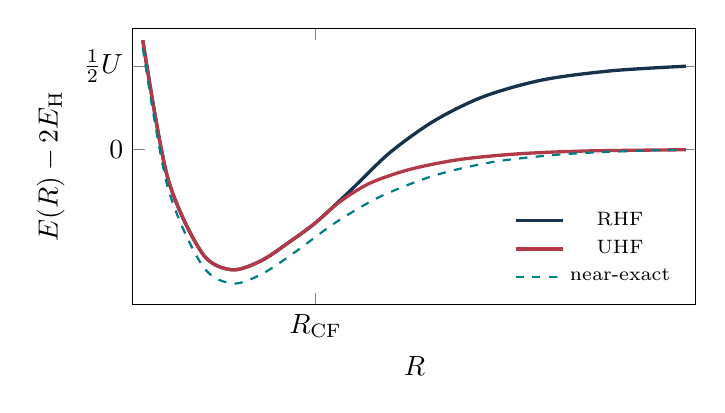
\begin{tikzpicture}
\begin{axis}[width=0.72\textwidth,height=0.42\textwidth,
xmin=0.45,xmax=6.15,ymin=-1.02,ymax=0.80,xlabel={$R$},
ylabel={$E(R)-2E_\text{H}$},xtick={2.30},xticklabels={$R_\text{CF}$},
ytick={0,0.55},yticklabels={$0$,$\tfrac12U$},
legend style={draw=none,fill=white,font=\scriptsize,
at={(0.98,0.03)},anchor=south east},clip=false]
\addplot[hfNavy,very thick,smooth] coordinates {
(0.55,0.72) (0.80,-0.18) (1.15,-0.68) (1.45,-0.79)
(1.75,-0.73) (2.05,-0.60) (2.30,-0.48) (2.65,-0.27)
(3.05,-0.02) (3.50,0.19) (4.00,0.35) (4.60,0.46)
(5.30,0.52) (6.05,0.55)};
\addlegendentry{RHF}
\addplot[hfRed,very thick,smooth] coordinates {
(0.55,0.72) (0.80,-0.18) (1.15,-0.68) (1.45,-0.79)
(1.75,-0.73) (2.05,-0.60) (2.30,-0.48) (2.55,-0.34)
(2.85,-0.22) (3.25,-0.13) (3.75,-0.065) (4.35,-0.027)
(5.05,-0.008) (6.05,0.00)};
\addlegendentry{UHF}
\addplot[hfTeal,thick,dashed,smooth] coordinates {
(0.55,0.67) (0.80,-0.24) (1.15,-0.76) (1.45,-0.88)
(1.75,-0.82) (2.10,-0.67) (2.50,-0.48) (2.95,-0.31)
(3.50,-0.17) (4.10,-0.080) (4.80,-0.030) (5.50,-0.008)
(6.05,0.00)};
\addlegendentry{near-exact}
\end{axis}
\end{tikzpicture}
\caption{Schematic RHF, UHF, and near-exact dissociation curves for
minimal-basis \ce{H2}.}
\label{fig:h2-dissociation}
\end{figure}

For the two-electron $M_S=0$ determinant,
\begin{equation}
  \boxed{
    \expval{\purple{\chS^2}}_\text{UHF}
    =1-\abs{\braket{\psi^\alpha}{\psi^\beta}}^2
    =\sin^2(2\theta)
  }.
\end{equation}
Near equilibrium, $\theta=0$ and $\expval*{\purple{\chS^2}}=0$, so the
determinant is a pure singlet. At dissociation, $\theta\rightarrow\pi/4$ and
$\expval*{\purple{\chS^2}}\rightarrow1$, so it is an equal mixture of a
singlet and an $M_S=0$ triplet:
\begin{equation}
  \ket{A\alpha\,B\beta}
  =\frac{1}{\sqrt2}\qty(
    \ket{\text{covalent singlet}}
    +\ket{\text{triplet},M_S=0})
  \qquad\text{as }R\to\infty.
\end{equation}
Thus, \red{the UHF energy is physically useful, but the UHF wavefunction is
spin-contaminated}. The three take-home messages are
\begin{enumerate}
  \item a stationary SCF solution need not be stable;
  \item the Coulson--Fischer point marks a continuous RHF-to-UHF transition;
  \item symmetry breaking mimics static correlation at the price of a
    contaminated wavefunction.
\end{enumerate}

The example exposes the characteristic compromise of broken-symmetry
mean-field theory. The determinant reproduces the correct separated-atom
energy through spin localization, but represents the singlet character only
through a mixture of spin eigenfunctions.

\subsection{Generalized Hartree--Fock theory}

Unrestricted Hartree--Fock remains collinear: every occupied orbital is either
purely $\alpha$ or purely $\beta$ with respect to one common quantization
axis. Generalized Hartree--Fock removes this remaining restriction. The key
idea is that GHF allows every orbital to choose its spin direction.
A GHF orbital is a \red{two-component spinor}:
\begin{equation}
  \boxed{
    \chi_p^\text{GHF}(\bx)
    =\alpha(\omega)\blue{\psi_p^\alpha(\br)}
    +\beta(\omega)\red{\psi_p^\beta(\br)}
  }.
\end{equation}
Both components are expanded in the same spatial AO basis,
\begin{equation}
  \psi_i^\sigma(\br)=\sum_{\mu=1}^{K}C_{\mu i}^\sigma\phi_\mu(\br),
  \qquad
  \boldsymbol{\mathcal C}=\mqty(\bC^\alpha\\\bC^\beta),
  \qquad
  \boldsymbol{\mathcal C}\in\mathbb C^{2K\times N}.
\end{equation}
RHF pairs electrons in one spatial orbital and preserves both
$\purple{\chS^2}$ and $\violet{\chS_z}$. UHF uses orbitals that are purely
$\alpha$ or $\beta$, has a collinear spin density, and preserves
$\violet{\chS_z}$. GHF permits each orbital to mix $\alpha$ and $\beta$, so
in general neither $\purple{\chS^2}$ nor $\violet{\chS_z}$ is preserved.
GHF therefore does not require a common spin-quantization axis or fixed values
of $N^\alpha$ and $N^\beta$.

RHF and UHF are consequently contained as special cases of GHF. A GHF
coefficient matrix has twice as many rows because every spatial basis function
can appear in both spin components of each occupied spinor.

\begin{figure}[htbp]
\centering
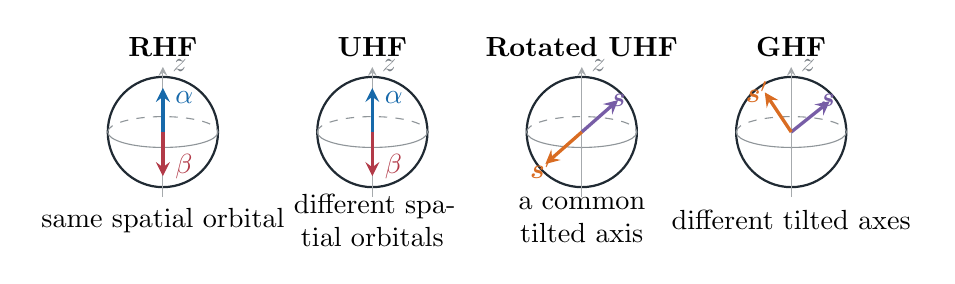
\begin{tikzpicture}[>=stealth,scale=0.70]
\foreach \x/\name/\desc in {
 -5.7/RHF/{same spatial orbital},
 -1.9/UHF/{different spatial orbitals},
  1.9/{Rotated UHF}/{a common tilted axis},
  5.7/GHF/{different tilted axes}}{
 \begin{scope}[shift={(\x,1.0)}]
  \draw[hfInk,thick] (0,0) circle (1.00);
  \draw[hfInk!50] (-1.00,0) arc (180:360:1.00 and 0.28);
  \draw[hfInk!50,dashed] (-1.00,0) arc (180:0:1.00 and 0.28);
  \draw[->,hfInk!40] (0,-1.18)--(0,1.18);
  \node[right,hfInk!60] at (0,1.2) {$z$};
 \end{scope}
 \node[above] at (\x,2.20) {\textbf{\name}};
 \node[align=center,text width=3.2cm] at (\x,-0.60) {\desc};
}
\draw[->,very thick,hfBlue] (-5.7,1.0)--(-5.7,1.80);
\draw[->,very thick,hfRed] (-5.7,1.0)--(-5.7,0.20);
\node[right,hfBlue] at (-5.65,1.62) {$\alpha$};
\node[right,hfRed] at (-5.65,0.38) {$\beta$};
\draw[->,very thick,hfBlue] (-1.9,1.0)--(-1.9,1.80);
\draw[->,very thick,hfRed] (-1.9,1.0)--(-1.9,0.20);
\node[right,hfBlue] at (-1.85,1.62) {$\alpha$};
\node[right,hfRed] at (-1.85,0.38) {$\beta$};
\draw[->,very thick,hfViolet] (1.9,1.0)--(2.56,1.58);
\draw[->,very thick,hfOrange] (1.9,1.0)--(1.24,0.42);
\node[above right,hfViolet] at (2.25,1.28) {$\boldsymbol{s}$};
\node[below left,hfOrange] at (1.55,0.72) {$\boldsymbol{s}'$};
\draw[->,very thick,hfViolet] (5.7,1.0)--(6.40,1.56);
\draw[->,very thick,hfOrange] (5.7,1.0)--(5.22,1.72);
\node[above right,hfViolet] at (6.05,1.28) {$\boldsymbol{s}$};
\node[above left,hfOrange] at (5.46,1.36) {$\boldsymbol{s}'$};
\end{tikzpicture}
\begin{equation}
 \underbrace{\text{UHF}\xrightarrow{\text{global spin rotation}}
 \text{rotated UHF}}_{\text{physically equivalent collinear solutions}}
 \qquad\neq\qquad
 \underbrace{\text{genuine GHF}}_{\text{non-collinear}}.
\end{equation}
\caption{RHF, UHF, globally rotated UHF, and genuinely noncollinear GHF spin
directions. A tilted spin axis alone does not imply a genuinely noncollinear
GHF solution.}
\label{fig:ghf-spin-directions}
\end{figure}

The GHF density matrix is
\begin{equation}
  \boxed{
    \boldsymbol{\mathcal P}=\mqty(
      \bP^{\alpha\alpha}&\bP^{\alpha\beta}\\
      \bP^{\beta\alpha}&\bP^{\beta\beta})
  },
  \qquad
  P_{\mu\nu}^{\sigma\sigma'}
  =\sum_{i=1}^{N}C_{\mu i}^\sigma C_{\nu i}^{\sigma' *}.
\end{equation}
The diagonal blocks describe the two collinear spin populations, whereas the
off-diagonal blocks encode coherence between the $\alpha$ and $\beta$
components. These off-diagonal blocks vanish for an ordinary UHF determinant.
Its charge and magnetization blocks are
\begin{align}
  \bP&=\frac12\qty(\bP^{\alpha\alpha}+\bP^{\beta\beta}),
  &
  \bM_z&=\frac12\qty(\bP^{\alpha\alpha}-\bP^{\beta\beta}),
  \\
  \bM_y&=\frac{1}{2\ii}\qty(\bP^{\beta\alpha}-\bP^{\alpha\beta}),
  &
  \bM_x&=\frac12\qty(\bP^{\beta\alpha}+\bP^{\alpha\beta}).
\end{align}
Equivalently,
\begin{equation}
  \boldsymbol{\mathcal P}
  =\mqty(
    \bP+\bM_z&\bM_x-\ii\bM_y\\
    \bM_x+\ii\bM_y&\bP-\bM_z)
  =\bP\otimes\bI+\bM\otimes\boldsymbol{\sigma},
\end{equation}
with
\begin{equation}
  \bM=\mqty(\bM_x\\\bM_y\\\bM_z),
  \qquad
  \boldsymbol{\sigma}
  =\mqty(\boldsymbol{\sigma}_x\\\boldsymbol{\sigma}_y\\
    \boldsymbol{\sigma}_z).
\end{equation}

The Roothaan--Hall equation in spinor space is
\begin{equation}
  \boxed{
    \boldsymbol{\mathcal F}\cdot\boldsymbol{\mathcal C}
    =\boldsymbol{\mathcal S}\cdot\boldsymbol{\mathcal C}
     \cdot\boldsymbol{\mathcal E}
  },
  \qquad
  \boldsymbol{\mathcal S}=\mqty(\bS&\bO\\\bO&\bS),
\end{equation}
with normalization
\begin{equation}
  \boldsymbol{\mathcal C}^\dagger\cdot\boldsymbol{\mathcal S}
  \cdot\boldsymbol{\mathcal C}=\bI.
\end{equation}
The GHF Fock matrix is
\begin{equation}
\boxed{
\boldsymbol{\mathcal F}=\mqty(
  \bh+\bJ[\bP^{\alpha\alpha}]+\bJ[\bP^{\beta\beta}]
    -\bK[\bP^{\alpha\alpha}]
  &-\bK[\bP^{\alpha\beta}]\\
  -\bK[\bP^{\beta\alpha}]
  &\bh+\bJ[\bP^{\alpha\alpha}]+\bJ[\bP^{\beta\beta}]
    -\bK[\bP^{\beta\beta}])
}
\end{equation}
where
\begin{equation}
  J_{\mu\nu}[\bP]
  =\sum_{\lambda\sigma}P_{\lambda\sigma}
    \rbraket{\mu\nu}{\lambda\sigma},
  \qquad
  K_{\mu\nu}[\bP]
  =\sum_{\lambda\sigma}P_{\lambda\sigma}
    \rbraket{\mu\sigma}{\lambda\nu}.
\end{equation}
The off-diagonal exchange blocks couple the $\alpha$ and $\beta$ components
self-consistently. The SCF procedure builds all four density blocks, builds
all four Fock blocks, solves a $2K\times2K$ generalized eigenvalue problem,
occupies the $N$ lowest spinors, and iterates.

The mathematical structure is the same nonlinear generalized eigenvalue
problem as before, now expressed in a doubled spinor space. The off-diagonal
exchange blocks are precisely the new terms that permit the spin direction to
rotate away from the common UHF axis.

For the corresponding global minima in the same one-electron basis,
\begin{equation}
  \boxed{
    \{\Phi_\text{RHF}\}\subset\{\Phi_\text{UHF}\}
    \subset\{\Phi_\text{GHF}\}
  }
  \qquad\Longrightarrow\qquad
  \red{E_\text{GHF}\leq E_\text{UHF}\leq E_\text{RHF}}.
\end{equation}
A converged UHF determinant may remain unstable to occupied-virtual rotations
that mix $\alpha$ and $\beta$ orbitals; following a negative-curvature
direction gives a lower-energy GHF solution. Not every GHF solution is
noncollinear: RHF and UHF are special cases, and a global spin rotation of a
UHF determinant changes its apparent quantization axis while remaining
physically collinear.

Lowering the variational energy may require breaking exact symmetries. UHF
may break $\chS^2$; GHF may break both $\chS^2$ and $\chS_z$; and complex GHF
may also break time-reversal symmetry. GHF remains a single determinant, so
correlation is not included, and $S$ and $M_S$ are generally not good quantum
numbers. The many stationary solutions make the initial guess and
\red{stability analysis} important. A putative GHF solution may be a globally
rotated UHF solution, requiring a \red{collinearity test}. Equilateral
\red{\ce{H3}} and \red{triangular magnetic clusters} are typical genuine
noncollinear examples. GHF is the most general \red{number-conserving}
single-determinant HF ansatz; particle-number symmetry can instead be broken
within \red{Hartree--Fock--Bogoliubov (HFB) theory}.

\subsection{Classification of Hartree--Fock solutions}

The labels RHF, UHF, and GHF describe broad variational classes, but each class
contains further possibilities depending on whether the orbitals are real or
complex and which spin and time-reversal symmetries are retained. The
Stuber--Paldus notation organizes these stationary solutions by symmetry and
by the block structure of their coefficient matrices.

The Stuber--Paldus classification is summarized in
Table~\ref{tab:stuber-paldus}.
\begin{table}[htbp]
\centering
\footnotesize
\setlength{\tabcolsep}{2.5pt}
\renewcommand{\arraystretch}{1.35}
\begin{tabular}{
  >{\centering\arraybackslash}m{0.14\textwidth}
  >{\centering\arraybackslash}m{0.19\textwidth}
  >{\centering\arraybackslash}m{0.17\textwidth}
  >{\centering\arraybackslash}m{0.39\textwidth}}
\rowcolor{hfPale}
\makecell{\textbf{Fukutome}\\\textbf{designation}}&
\makecell{\textbf{Stuber--Paldus}\\\textbf{designation}}&
\makecell{\textbf{Symmetries}\\\textbf{preserved}}&
\makecell{\textbf{Structure of the orbital}\\
          \textbf{coefficient matrix $\bC$}}\\
$\text{TICS}^{a}$&real RHF&$\chS^2,\chS_z,\chK,\hat\Theta$&
$\mqty(\bC_{\sigma\sigma}&\bO\\\bO&\bC_{\sigma\sigma}),
\ \bC\in\mathbb R$\\
$\text{CCW}^{b}$&complex RHF&$\chS^2,\chS_z$&
$\mqty(\bC_{\sigma\sigma}&\bO\\\bO&\bC_{\sigma\sigma})$\\
$\text{ASCW}^{c}$&paired UHF&$\chS_z,\hat\Theta$&
$\mqty(\bC_{\sigma\sigma}&\bO\\\bO&\bC_{\sigma\sigma}^*)$\\
$\text{ASDW}^{d}$&real UHF&$\chS_z,\chK$&
$\mqty(\bC_{\sigma\sigma}&\bO\\\bO&\bC_{\sigma'\sigma'}),
\ \bC\in\mathbb R$\\
$\text{ASW}^{e}$&complex UHF&$\chS_z$&
$\mqty(\bC_{\sigma\sigma}&\bO\\\bO&\bC_{\sigma'\sigma'})$\\
$\text{TSCW}^{f}$&paired GHF&$\hat\Theta$&
$\mqty(\bC_{\sigma\sigma}&\bC_{\sigma\sigma'}\\
-\bC_{\sigma\sigma'}^*&\bC_{\sigma\sigma}^*)$\\
$\text{TSDW}^{g}$&real GHF&$\chK$&
$\mqty(\bC_{\sigma\sigma}&\bC_{\sigma\sigma'}\\
\bC_{\sigma'\sigma}&\bC_{\sigma'\sigma'}),\ \bC\in\mathbb R$\\
$\text{TSW}^{h}$&complex GHF&---&
$\mqty(\bC_{\sigma\sigma}&\bC_{\sigma\sigma'}\\
\bC_{\sigma'\sigma}&\bC_{\sigma'\sigma'})$
\end{tabular}
\caption{Stuber--Paldus classification of Hartree--Fock solutions.}
\label{tab:stuber-paldus}
\end{table}

Here TICS denotes time-reversal-invariant closed-shell; CCW, charge current
wave; ASCW, axial spin current wave; ASDW, axial spin density wave; ASW,
axial spin wave; TSCW, torsional spin current wave; TSDW, torsional spin
density wave; and TSW, torsional spin wave. The operators $\chK$ and
$\hat\Theta$ are complex conjugation and time reversal, respectively.

\begin{figure}[htbp]
  \centering
  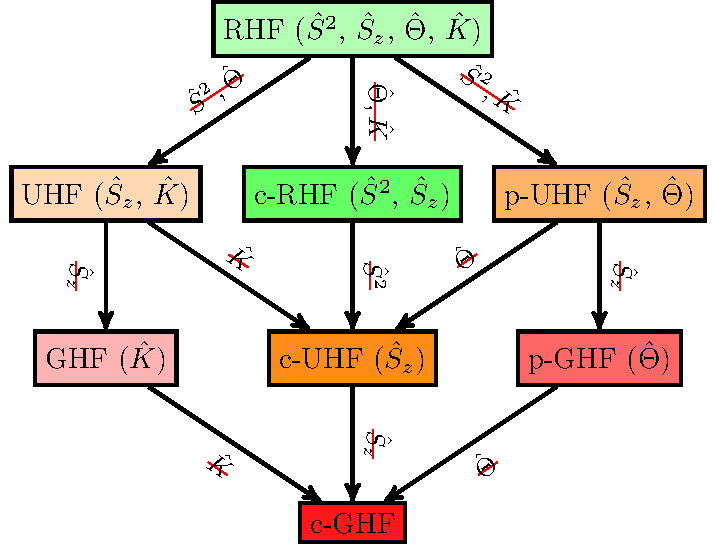
\includegraphics[width=0.66\textwidth]{StuberPaldus}
  \caption{Graphical Stuber--Paldus classification of Hartree--Fock
  solutions.}
  \label{fig:stuber-paldus}
\end{figure}

The table makes the variational hierarchy concrete. Moving from restricted to
unrestricted and then generalized orbitals removes constraints from the
coefficient matrix; allowing complex coefficients removes additional
antiunitary symmetries. These larger spaces can contain lower stationary
energies, but identifying their physical symmetry requires examining the
solution rather than relying only on its numerical energy.

\section{Further reading on Hartree--Fock theory}

The books recommended in the slides are
\begin{itemize}
  \item \emph{Introduction to Computational Chemistry}, Jensen;
  \item \emph{Essentials of Computational Chemistry}, Cramer;
  \item \emph{Modern Quantum Chemistry}, Szabo and Ostlund;
  \item \emph{Molecular Electronic Structure Theory}, Helgaker, J{\o}rgensen,
    and Olsen.
\end{itemize}
\begin{center}
  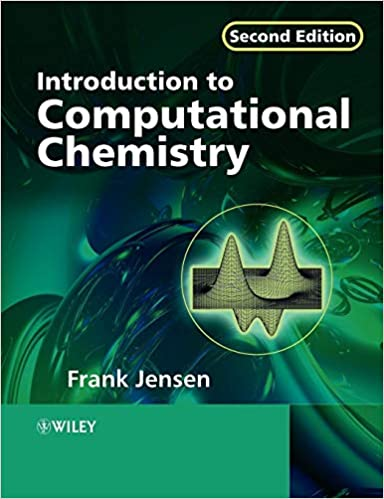
\includegraphics[height=0.12\textheight]{Jensen}\hspace{1em}
  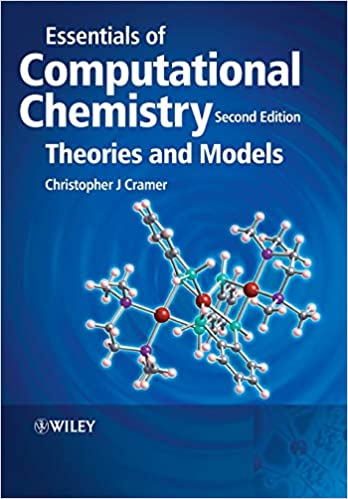
\includegraphics[height=0.12\textheight]{Cramer}\hspace{1em}
  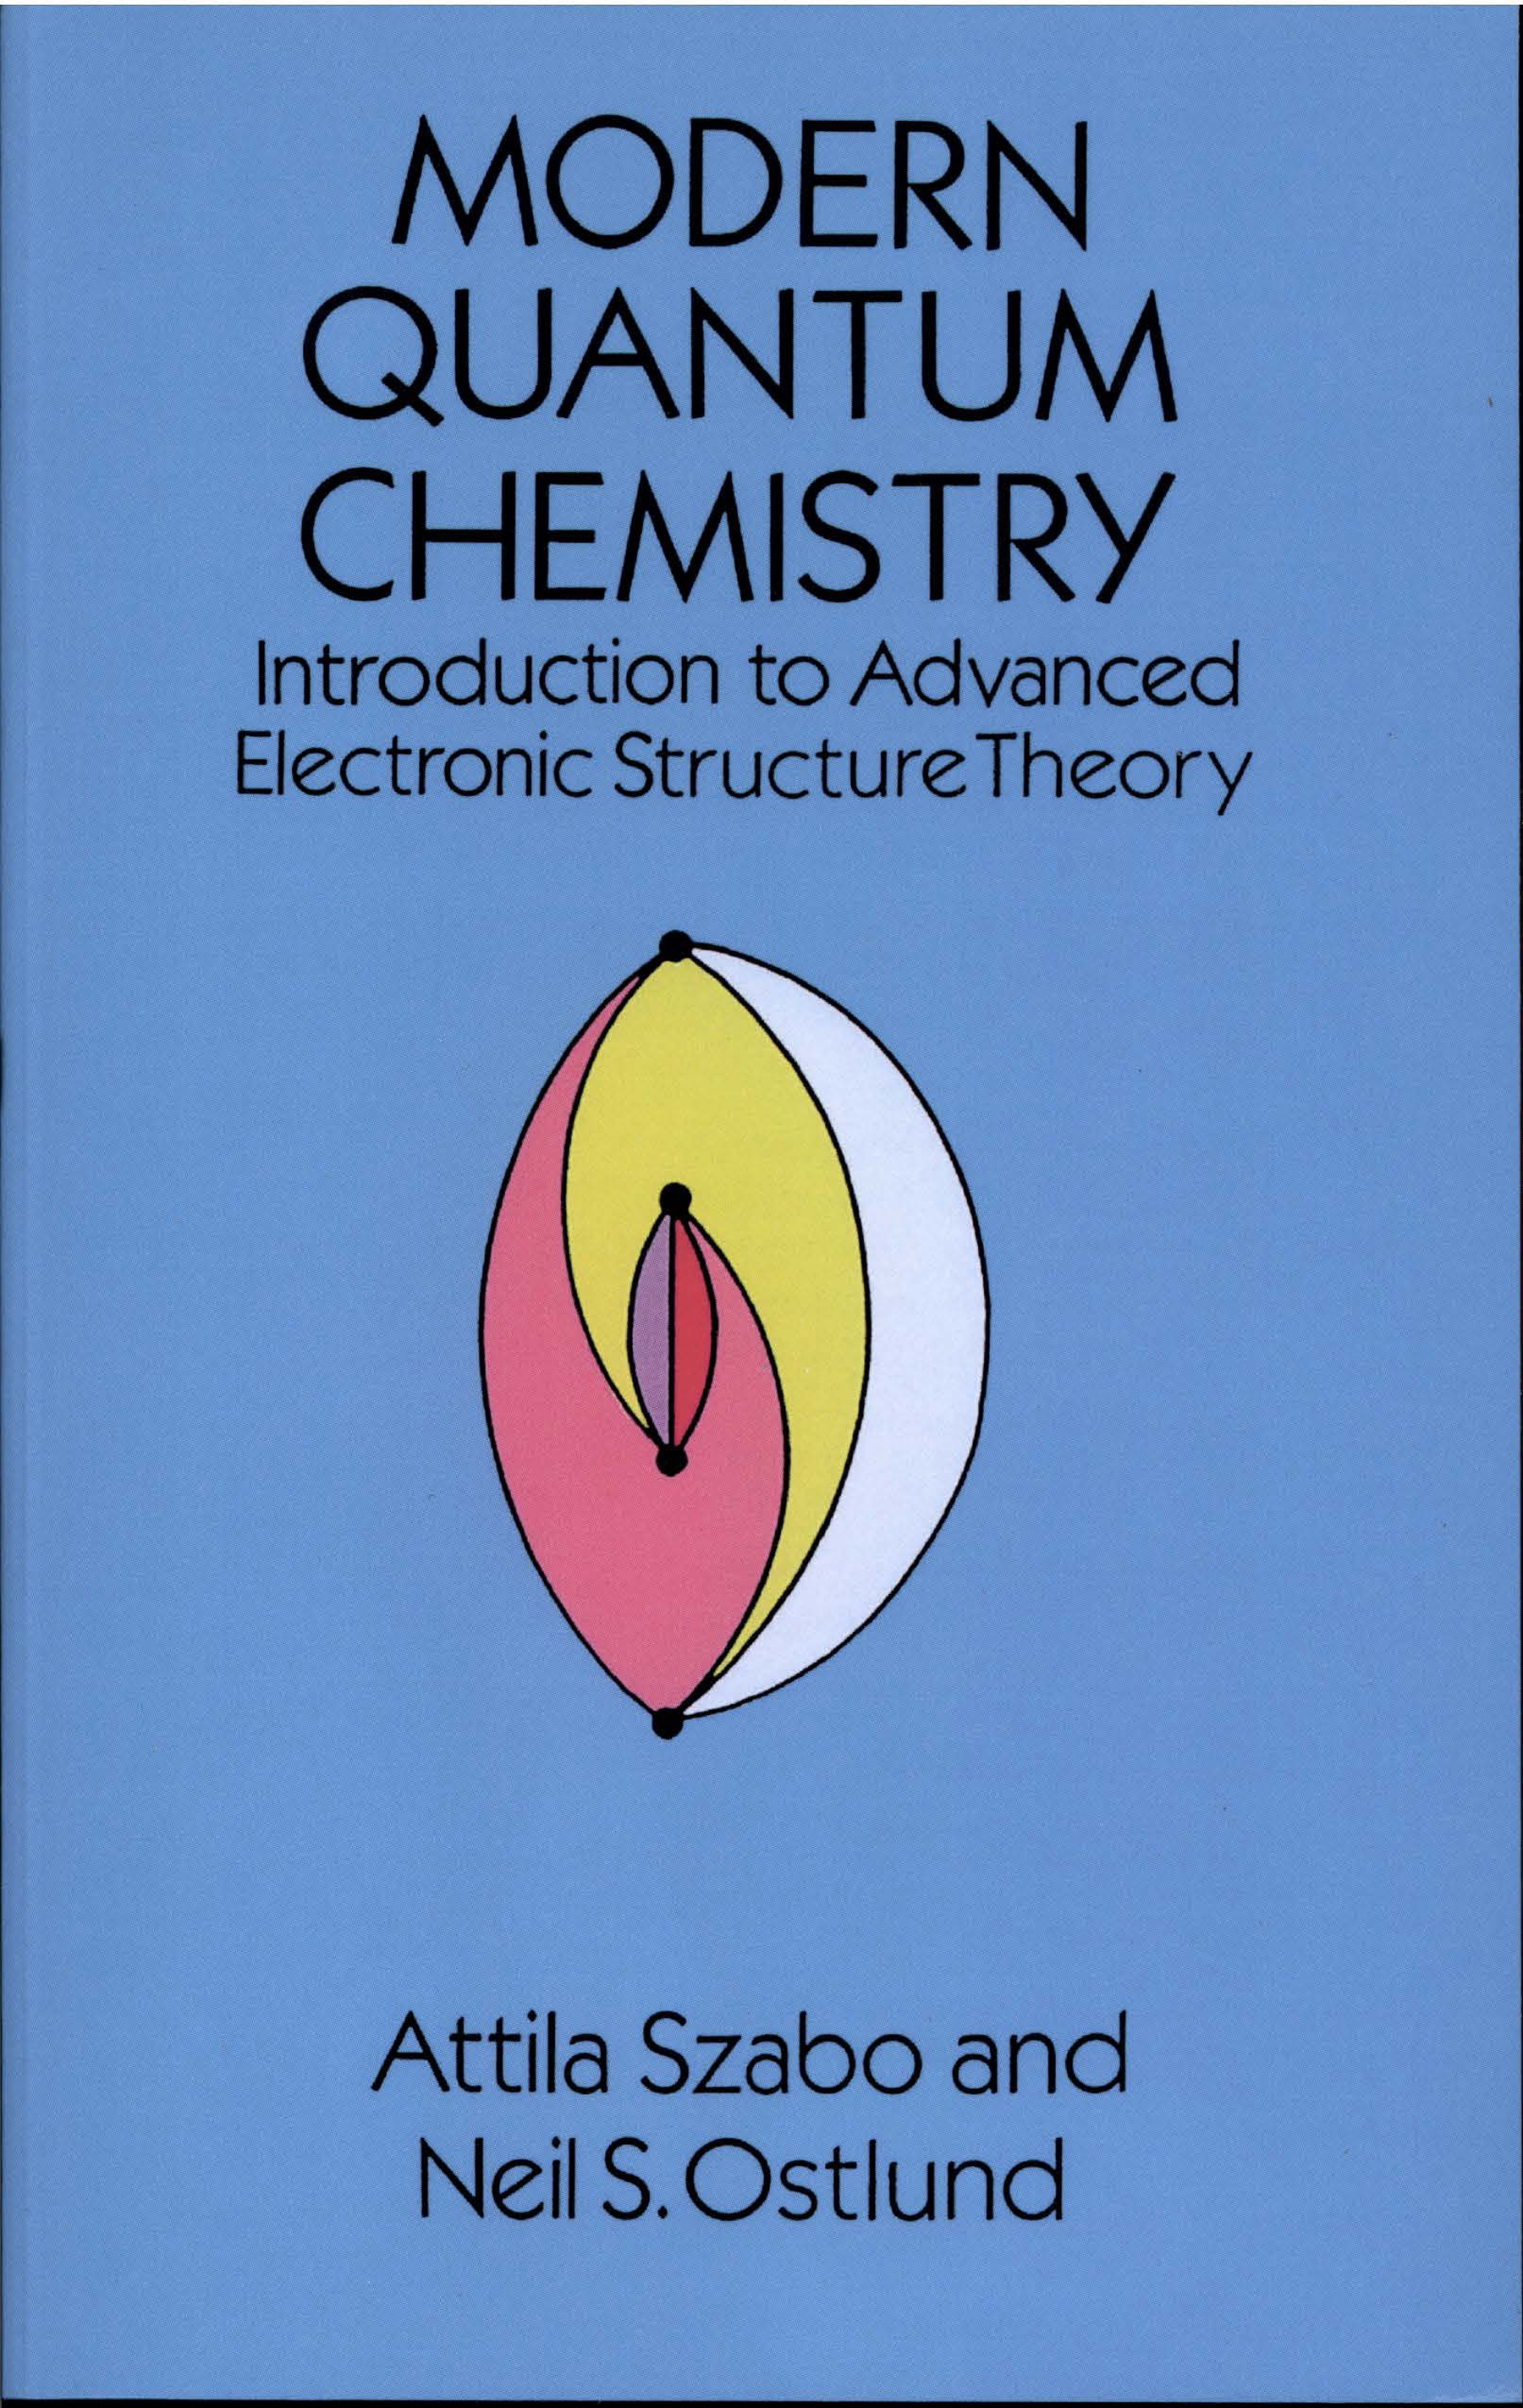
\includegraphics[height=0.12\textheight]{Szabo}\hspace{1em}
  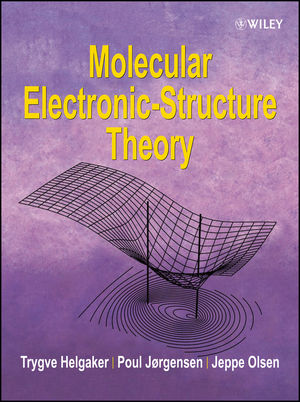
\includegraphics[height=0.12\textheight]{Helgaker}
\end{center}

% ============================================================================
% Presentation II: ESQC_Loos_BF.tex
% The presentation has no explicit LaTeX section hierarchy; its content is
% organized below in the original frame order.
% ============================================================================

\clearpage
\section{One-electron basis sets}

\subsection{Expanding molecular orbitals}

In practical molecular calculations, each molecular orbital is expanded in a
finite set of known one-electron functions,
\begin{equation}
  \boxed{\psi_p(\br)=\sum_{\mu=1}^{K}C_{\mu p}\phi_\mu(\br)}.
\end{equation}
The basis functions $\phi_\mu$ are fixed, whereas the coefficients $C_{\mu p}$
are determined variationally. Increasing $K$ systematically enlarges the
variational space and moves the result toward the complete-basis-set (CBS)
limit. Consequently, the basis set is the only source of empirical parameters
in an otherwise ab initio calculation.

A useful basis must be accurate, compact, numerically stable, and practical.
These requirements compete: a larger and more flexible basis improves the
description of the orbitals, but increases both the computational cost and the
risk of linear dependence.

\paragraph{The LEGO principle.}

Basis-set construction follows a LEGO-like philosophy: a small collection of
well-designed building blocks is combined to describe chemically diverse
systems.
\begin{figure}[htbp]
  \centering
  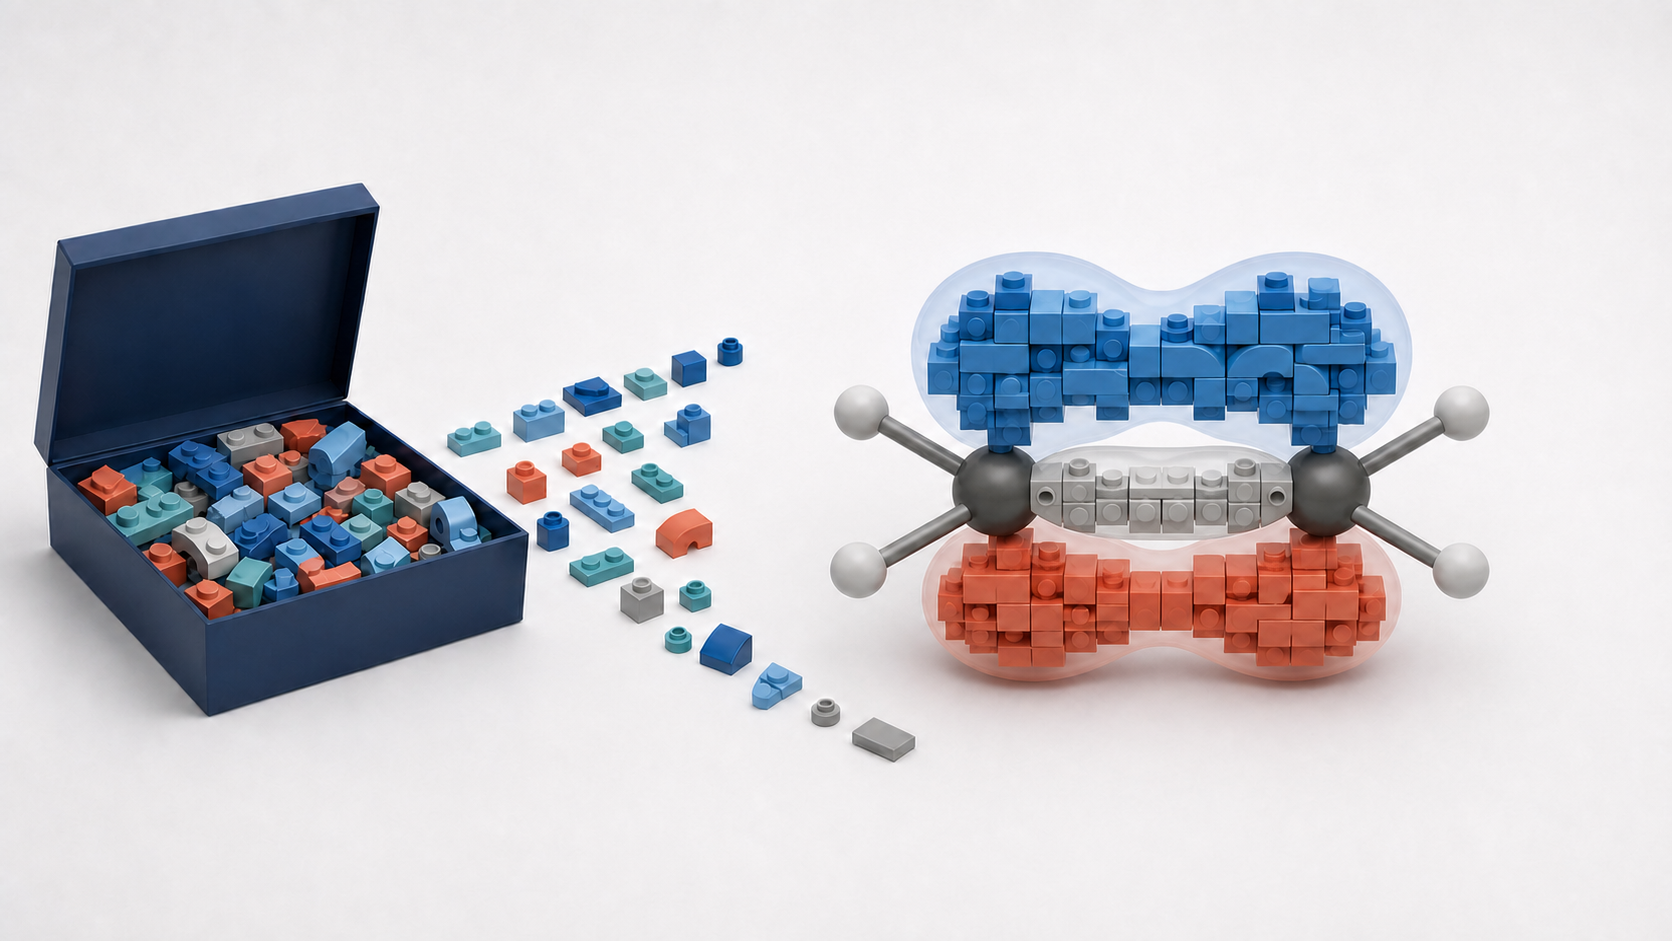
\includegraphics[width=0.62\textwidth]{lego}
  \caption{The basis functions are the elementary building blocks from which
  molecular orbitals are assembled.}
\end{figure}

\subsubsection{Common basis functions}

Several families of one-electron functions are routinely used.
\begin{itemize}
  \item \red{Gaussian-type orbitals (GTOs)}, proportional to
  $\exp(-\alpha r^2)$, are atom centered and are the standard choice for
  molecules. Their multicenter integrals are efficient. They are used in, for
  example, \textsc{Orca}, \textsc{Q-Chem}, \textsc{Molcas}, \textsc{Molpro},
  \textsc{PySCF}, \textsc{Psi4}, \textsc{CFOUR}, \textsc{MRCC}, and
  \textsc{GAMESS}.
  \item \blue{Slater-type orbitals (STOs)}, proportional to
  $\exp(-\zeta r)$, are atom centered and have the correct nuclear cusp and
  long-range tail. They are used, for example, in \textsc{ADF}.
  \item \orange{Plane waves (PWs)}, proportional to $\exp(\ii\bk\cdot\br)$,
  are delocalized, mutually orthonormal, and naturally adapted to periodic
  boundary conditions. Their size is controlled by an energy cutoff. They are
  used in \textsc{Quantum Espresso}, \textsc{VASP}, \textsc{ABINIT}, and
  \textsc{CASTEP}.
  \item \green{Numerical atomic orbitals (NAOs)} have tabulated radial parts.
  They are compact and flexible and are used in \textsc{FHI-aims} and
  \textsc{SIESTA}.
\end{itemize}

\subsection{Plane waves}

In a unit cell of volume $\Omega$, a normalized plane wave is
\begin{equation}
  \phi_{\bk}(\br)=\frac{1}{\sqrt{\Omega}}\exp(\ii\bk\cdot\br),
  \qquad \abs{\bk}\leq k_\text{cut},
  \qquad E_\text{cut}=\frac{k_\text{cut}^2}{2}.
\end{equation}
The reciprocal-lattice vector is
\begin{equation}
  \bk=k_1\bb_1+k_2\bb_2+k_3\bb_3,
\end{equation}
where, for direct-lattice vectors $\ba_1,\ba_2,\ba_3$,
\begin{align}
  \Omega&=\ba_1\cdot(\ba_2\times\ba_3),
  &\bA&=(\ba_1,\ba_2,\ba_3),\\
  \bb_1&=2\pi\frac{\ba_2\times\ba_3}{\Omega},
  &\bb_2&=2\pi\frac{\ba_3\times\ba_1}{\Omega},
  &\bb_3&=2\pi\frac{\ba_1\times\ba_2}{\Omega}.
\end{align}

The overlap integrals are diagonal:
\begin{align}
  \braket{\bk_1}{\bk_2}
  &=\frac{1}{\Omega}\int_\Omega
    \exp[-\ii\bk_1\cdot\br]\exp[\ii\bk_2\cdot\br]\dd\br\\
  &=\frac{1}{\Omega}\int_\Omega
    \exp[\ii(\bk_2-\bk_1)\cdot\br]\dd\br
  =\delta_{\bk_1\bk_2}.
\end{align}
The kinetic-energy integrals are diagonal as well:
\begin{align}
  \mel{\bk_1}{-\frac12\nabla^2}{\bk_2}
  &=\frac{1}{\Omega}\int_\Omega
    \exp[-\ii\bk_1\cdot\br]
    \qty(-\frac12\nabla^2)\exp[\ii\bk_2\cdot\br]\dd\br\\
  &=\frac{k_2^2}{2\Omega}\int_\Omega
    \exp[\ii(\bk_2-\bk_1)\cdot\br]\dd\br
  =\frac{k_2^2}{2}\delta_{\bk_1\bk_2}.
\end{align}
The electron-repulsion integral begins as
\begin{align}
  \rbraket{\bk_1\bk_2}{\bk_3\bk_4}
  &=\frac{1}{\Omega^2}\iint_\Omega
  \frac{\exp[\ii(\bk_3-\bk_1)\cdot\br_1]
        \exp[\ii(\bk_4-\bk_2)\cdot\br_2]}
       {r_{12}}\dd\br_1\dd\br_2.
\end{align}
Using the reciprocal-space resolution of the Coulomb operator,
\begin{equation}
  \frac{1}{r_{12}}=\frac{1}{\Omega}\sum_{\bk\ne\bO}
  \frac{4\pi}{k^2}\exp[\ii\bk\cdot(\br_1-\br_2)],
\end{equation}
where the $\bk=\bO$ term is delicate but can be treated, gives
\begin{align}
  \rbraket{\bk_1\bk_2}{\bk_3\bk_4}
  &=\frac{1}{\Omega^3}\sum_{\bk\ne\bO}\frac{4\pi}{k^2}
  \iint_\Omega\exp[\ii(\bk_3-\bk_1-\bk)\cdot\br_1]
  \exp[\ii(\bk_4-\bk_2+\bk)\cdot\br_2]\dd\br_1\dd\br_2\\
  &=\frac{1}{\Omega}\sum_{\bk\ne\bO}\frac{4\pi}{k^2}
  \delta_{\bk_3-\bk_1-\bk,\bO}
  \delta_{\bk_4-\bk_2+\bk,\bO}\\
  &=\frac{4\pi}{\Omega\abs{\bk_1-\bk_3}^2}
  \delta_{\bk_1+\bk_2,\bk_3+\bk_4}.
\end{align}
The Kronecker delta expresses conservation of crystal momentum.

The key physical picture is that assemblies of atoms are treated as slight
distortions of free electrons. Plane waves are orthonormal and independent of
the atomic positions; naturally compatible with periodic boundary conditions;
systematically convergent through the single parameter $E_\text{cut}$; and
diagonalize the kinetic and Coulomb operators in reciprocal space. They also
permit efficient fast-Fourier-transform evaluation and have neither basis-set
superposition error nor atom-centered Pulay forces. Their limitations are
large basis sizes,
\begin{equation}
  N_\text{PW}\propto\Omega E_\text{cut}^{3/2}.
\end{equation}
Core orbitals require prohibitively large cutoffs, motivating
pseudopotentials; the cost increases with supercell size; delocalized functions
provide little real-space sparsity; and the large virtual spaces make
correlated methods expensive.
Plane waves are therefore especially effective for periodic valence-electron
calculations, usually in conjunction with pseudopotentials.

\subsection{Slater and Gaussian orbitals}

The general Slater- and Gaussian-type orbitals used in the comparison are
\begin{equation}
 \boxed{\phi_{\zeta n\ell m}^\text{STO}(\br)
 \propto r^{n-1}e^{-\zeta r}Y_{\ell m}(\hat{\br})},
 \qquad
 \boxed{\phi_{\alpha n\ell m}^\text{GTO}(\br)
 \propto r^{2(n-1)-\ell}e^{-\alpha r^2}Y_{\ell m}(\hat{\br})}.
\end{equation}
For their $1s$ representatives, the STO has the correct nuclear cusp,
\begin{equation}
 \phi_\text{1s}^\text{STO}(r)\propto e^{-\zeta r},
 \qquad
 \eval{\dv{\phi_\text{1s}^\text{STO}(r)}{r}}_{r=0}=-\zeta,
\end{equation}
whereas the GTO is flat at the nucleus,
\begin{equation}
 \phi_\text{1s}^\text{GTO}(r)\propto e^{-\alpha r^2},
 \qquad
 \eval{\dv{\phi_\text{1s}^\text{GTO}(r)}{r}}_{r=0}=0.
\end{equation}
The STO also has the correct exponential long-range behavior of a molecular
orbital,
\begin{equation}
 \phi_\text{HOMO}^\text{STO}(r)
 \propto e^{-\sqrt{-2\epsilon_\text{HOMO}}r},
 \qquad \mathrm{IP}=-\epsilon_\text{HOMO}.
\end{equation}
A Gaussian instead decays too rapidly. Multicenter STO integrals are hard to
compute, whereas multicenter GTO integrals are easy. GTOs usually win, but more
of them are required.

\subsubsection{Primitive and contracted Gaussians}

A primitive Cartesian Gaussian centered at $\bA$ is
\begin{equation}
  \sket{\ba}=(x-A_x)^{a_x}(y-A_y)^{a_y}(z-A_z)^{a_z}
  \exp[-\alpha\abs{\br-\bA}^2].
\end{equation}
A contracted Gaussian is a fixed linear combination of primitives,
\begin{equation}
  \boxed{
  \ket{\ba}\equiv\phi_{\ba}^{\bA}(\br)
  =\sum_{k=1}^{K}D_k\sket{\ba_k}}.
\end{equation}
Here $\alpha$ is the exponent, $\bA$ the center, and
$\ba=(a_x,a_y,a_z)$ the angular-momentum vector, with total angular momentum
$a=a_x+a_y+a_z$.

An $s$ shell contains $(0,0,0)$; a $p$ shell contains $(1,0,0)$,
$(0,1,0)$, and $(0,0,1)$; a Cartesian $d$ shell contains
$(2,0,0)$, $(0,2,0)$, $(0,0,2)$, $(1,1,0)$, $(1,0,1)$, and $(0,1,1)$;
and a Cartesian $f$ shell contains
\begin{equation}
 \begin{gathered}
 (3,0,0),(0,3,0),(0,0,3),(2,1,0),(2,0,1),\\
 (1,2,0),(0,2,1),(0,1,2),(1,0,2),(1,1,1).
 \end{gathered}
\end{equation}
In general,
\begin{equation}
  N_\ell^\text{cart}=\frac{(\ell+1)(\ell+2)}{2},
\end{equation}
which gives $1,3,6,10$ functions for $s,p,d,f$. Spherical harmonics instead
give $N_\ell^\text{sph}=2\ell+1$, namely $1,3,5,7$. Thus
\begin{equation}
  6d=5d+1s,
  \qquad
  10f=7f+3p,
\end{equation}
because, for example, $x^2+y^2+z^2=r^2$. Most molecular calculations use
pure spherical functions.

Contraction reduces the number of variational coefficients, but it does not
remove the primitive-integral work. For four contracted functions,
\begin{equation}
  \rbraket{\ba\bb}{\bc\bd}
  =\sum_{i=1}^{K_a}\sum_{j=1}^{K_b}\sum_{k=1}^{K_c}\sum_{l=1}^{K_d}
  D_i^aD_j^bD_k^cD_l^d
  \sbraket{\ba_i\bb_j}{\bc_k\bd_l}.
\end{equation}
For example, a cc-pVTZ carbon $1s$ function contracted from ten primitives
requires $10^4$ primitive $ssss$ integrals for a single four-center integral.
\begin{figure}[htbp]
  \centering
  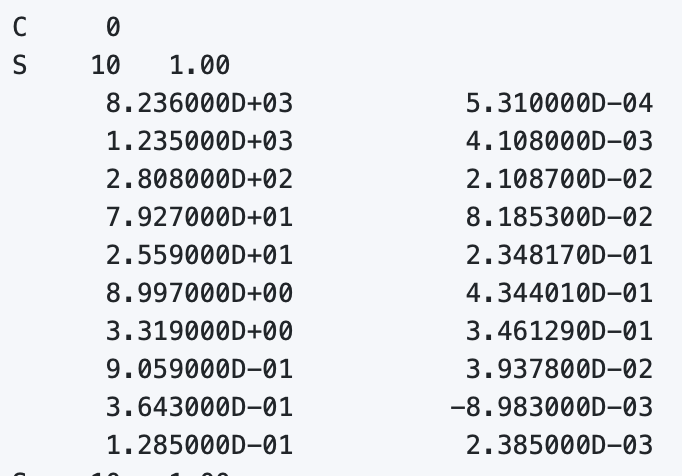
\includegraphics[width=0.62\textwidth]{C}
  \caption{Contracted Gaussian functions for carbon.}
\end{figure}
Basis-set definitions can be inspected and downloaded from the
\href{https://www.basissetexchange.org}{Basis Set Exchange}.

\subsection{Choosing a Gaussian basis}

Different physical effects demand different forms of flexibility.
\begin{itemize}
  \item \red{Radial flexibility} is provided by multiple-$\zeta$ functions,
  for example double-$\zeta$, triple-$\zeta$, and quadruple-$\zeta$ bases.
  \item \blue{Angular flexibility} is supplied by polarization functions,
  such as $d$ functions on second-row atoms and $p$ functions on hydrogen.
  \item \orange{Long-range flexibility} is supplied by diffuse functions
  with small exponents, which are important for anions, Rydberg states,
  noncovalent interactions, multipoles, and (hyper)polarizabilities.
  \item \green{Core flexibility} is supplied by tight functions and is needed
  for core correlation, nuclear magnetic shielding, and spin--spin coupling
  constants.
\end{itemize}

\begin{figure}[htbp]
  \centering
  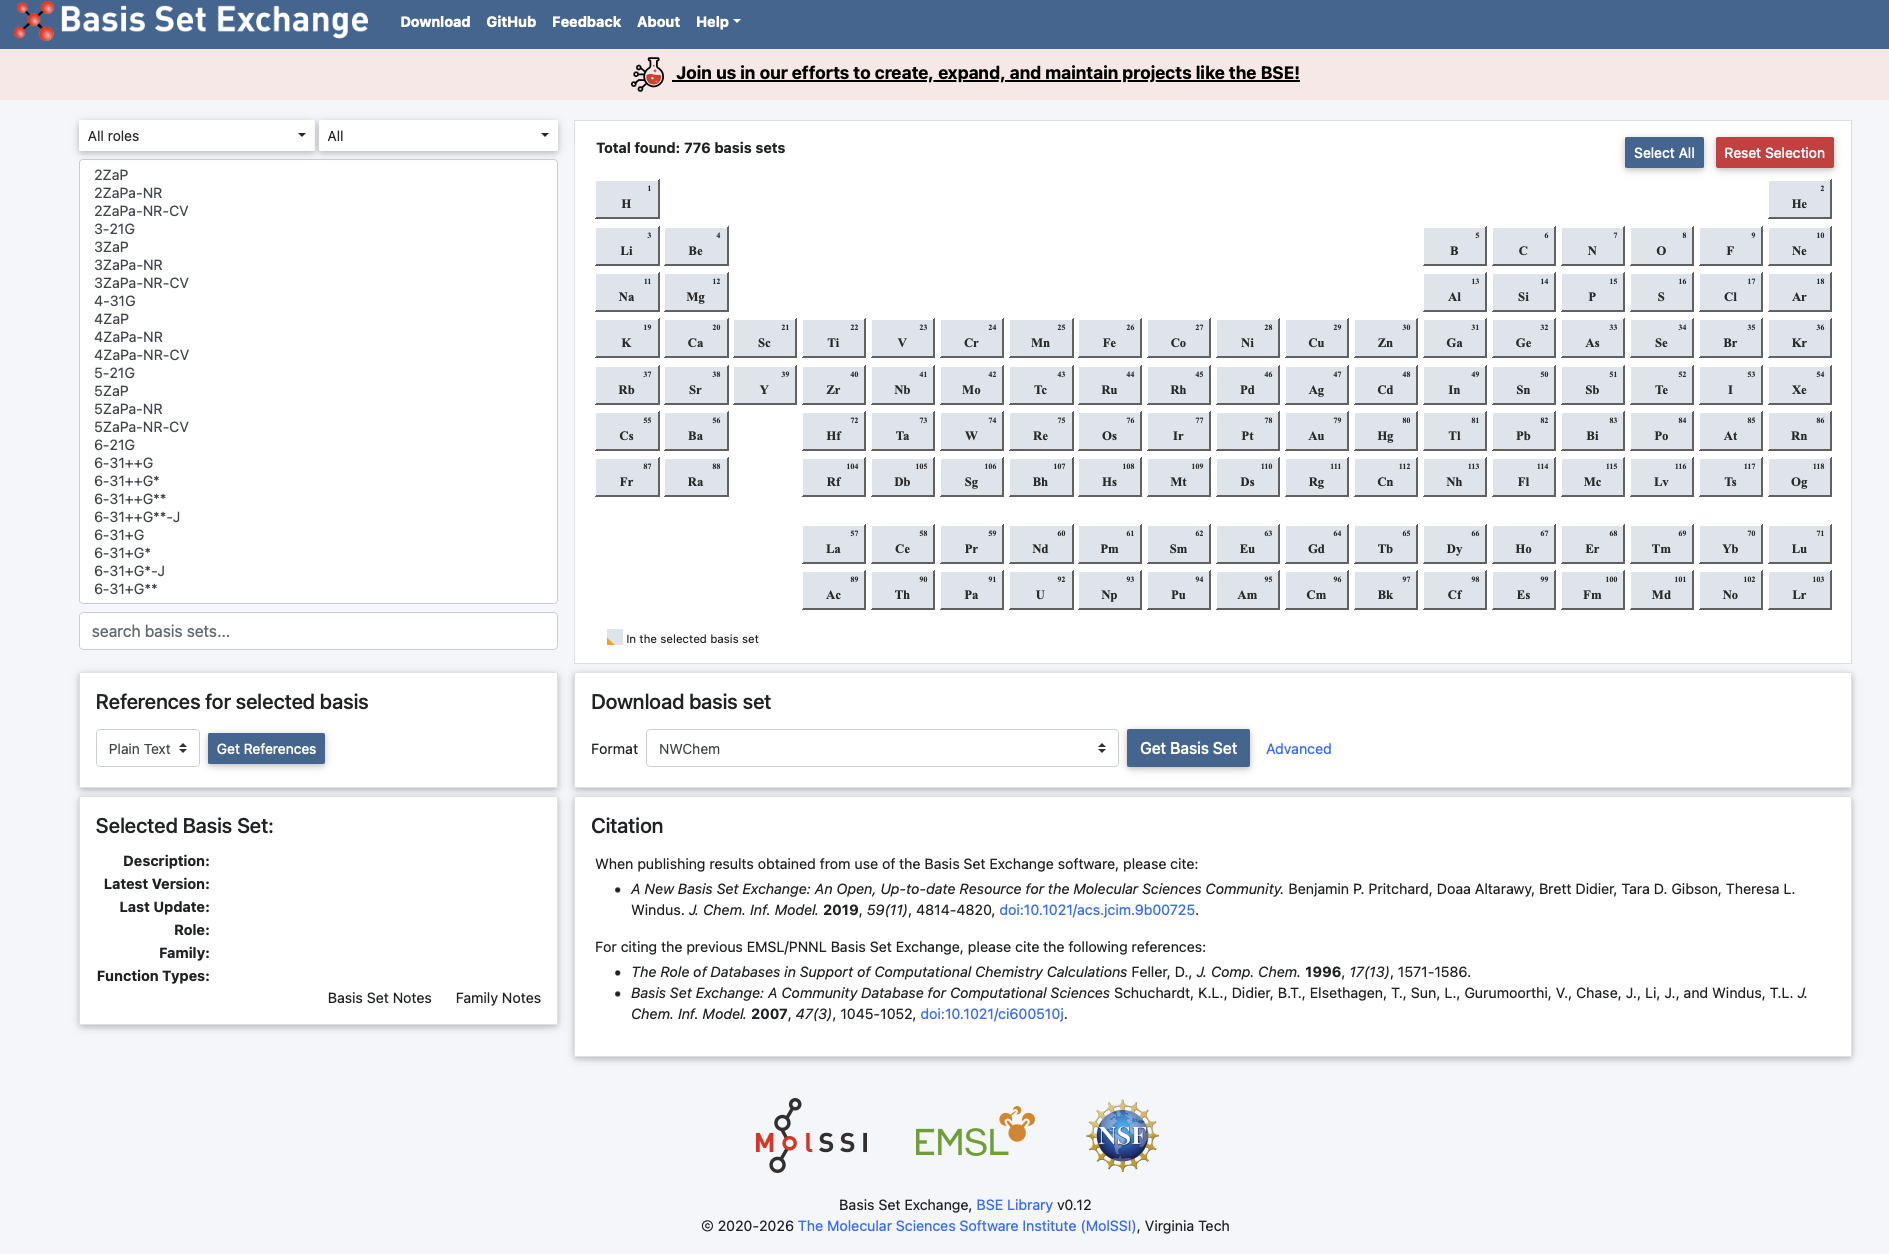
\includegraphics[width=0.72\textwidth]{BSE}
  \caption{The Basis Set Exchange provides standardized definitions for a
  large number of orbital and auxiliary basis sets.}
\end{figure}

\paragraph{STO-$n$G.}

In an STO-$n$G basis, there is one contracted basis function for every occupied
orbital in the minimal atomic description. Each contracted GTO contains $n$
primitive GTOs, whose contraction coefficients and exponents are selected so
that the contraction approximates an STO. STO-$n$G bases are therefore minimal,
single-$\zeta$ basis sets; STO-3G is the most familiar member.
\begin{center}
  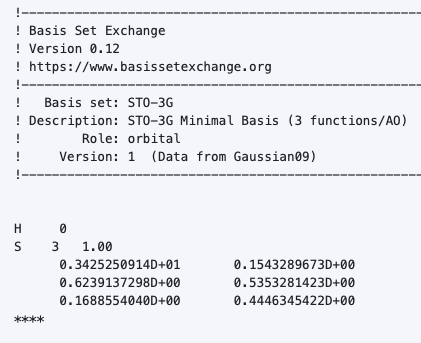
\includegraphics[width=0.42\textwidth]{STO-3G}\hspace{1em}
  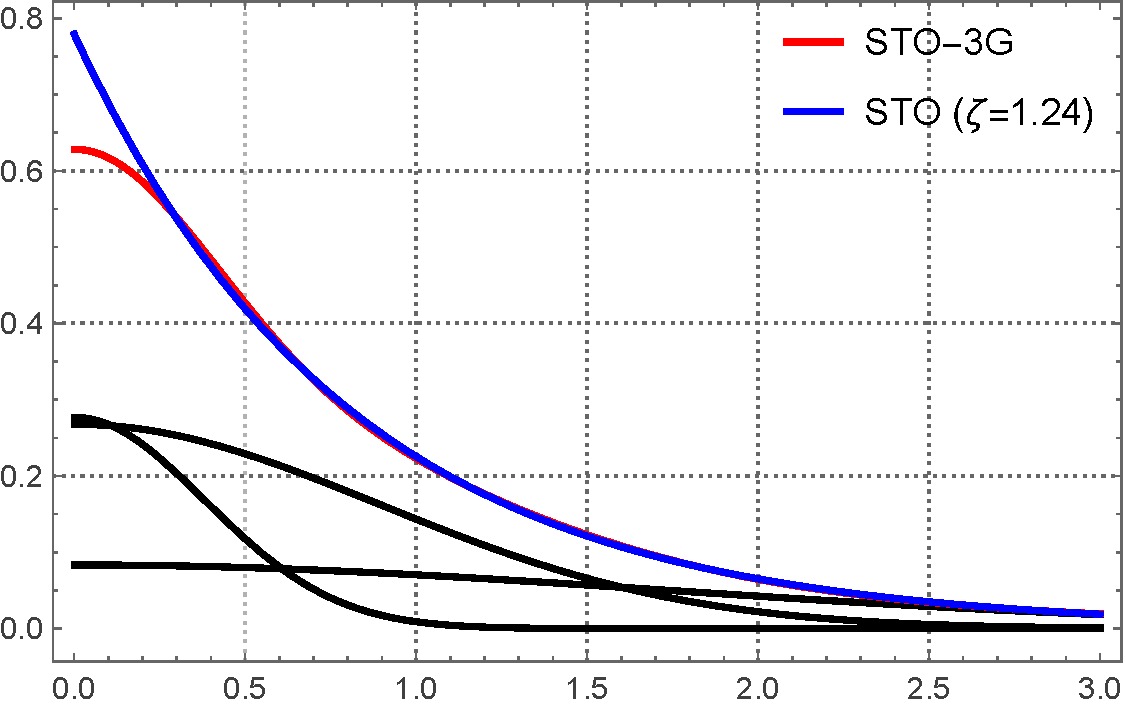
\includegraphics[width=0.42\textwidth]{STO}
\end{center}

\paragraph{Pople basis sets.}

The notation explicitly records the contractions and augmentations. In
6-31+G*, the core function is contracted from six primitives; the valence
space is double-$\zeta$, with contractions of three and one primitives; the
``+'' adds diffuse functions to non-hydrogen atoms; and ``*'' adds polarization
functions to non-hydrogen atoms, conventionally a $d$ shell. In 6-311++G**,
the valence space is triple-$\zeta$ with contractions $3,1,1$; the second
``+'' adds diffuse functions to hydrogen; and the second ``*'' adds
polarization functions to hydrogen. Finally, 6-311G(2df,2pd) adds two $d$ and
one $f$ polarization shells to non-hydrogen atoms, and two $p$ and one $d$
shell to hydrogen.

\paragraph{Dunning correlation-consistent basis sets.}

The main sequence is
\begin{equation}
  \boxed{\text{cc-pVXZ},\qquad X=\mathrm{D,T,Q,5,6}}.
\end{equation}
These bases were designed for correlated calculations, with balanced layers
of polarization functions and a systematically increasing valence space. A
standard correlation-energy extrapolation is
\begin{equation}
  \Ec(X)\approx\Ec^\text{CBS}+AX^{-3}.
\end{equation}
Diffuse augmentation gives aug-cc-pVXZ, d-aug-cc-pVXZ, and t-aug-cc-pVXZ.
Core correlation is described by cc-pCVXZ, optimized for core--core and
core--valence correlation, or by cc-pwCVXZ, which weights the core--valence
contribution.

For a second-row atom, the valence correlation-consistent sequence is
\begin{center}
\begin{tabular}{c@{\qquad}c}
\toprule
Basis & shell content\\
\midrule
cc-pVDZ & $3s2p1d$\\
cc-pVTZ & $4s3p2d1f$\\
cc-pVQZ & $5s4p3d2f1g$\\
aug-cc-pVDZ & $4s3p2d$\\
aug-cc-pVTZ & $5s4p3d2f$\\
aug-cc-pVQZ & $6s5p4d3f2g$\\
d-aug-cc-pVDZ & $5s4p3d$\\
d-aug-cc-pVTZ & $6s5p4d3f$\\
d-aug-cc-pVQZ & $7s6p5d4f3g$\\
\bottomrule
\end{tabular}
\end{center}
The successive entries make the layered construction explicit. For the
core--valence sequence, the corresponding decomposition is
\begin{align}
 \text{cc-pVDZ: }&3s2p1d=1s+2s2p1d,\\
 \text{cc-pVTZ: }&4s3p2d1f=1s+3s3p2s1f,\\
 \text{cc-pVQZ: }&5s4p3d2f1g=1s+4s4p3d2f1g,\\
 \text{cc-pCVDZ: }&4s3p1d=2s1p+2s2p1d,\\
 \text{cc-pCVTZ: }&6s5p3d1f=3s2p1d+3s3p2d1f,\\
 \text{cc-pCVQZ: }&8s7p5d3f1g=4s3p2d1f+4s4p3d2f1g.
\end{align}

\paragraph{Jensen polarization-consistent basis sets.}

The sequence has shell contents
\begin{equation}
  \text{pc-0}:3s2p,quad
  \text{pc-1}:3s2p1d,quad
  \text{pc-2}:4s3p2d1f,quad
  \text{pc-3}:6s5p4d2f1g.
\end{equation}
Thus pc-0 is unpolarized, pc-1 adds one polarization layer, and the later
members add systematically more radial and angular flexibility. These basis
sets were designed for HF and Kohn--Sham calculations, with higher angular
momenta selected according to their energetic importance. Diffuse variants
are denoted aug-pc-$n$. Their HF convergence is described by
\begin{equation}
  \boxed{E_\text{HF}(L)=E_\text{HF}^\text{CBS}
  +A(L+1)\exp(-B\sqrt L)}.
\end{equation}

Gaussian bases are compact, atom centered, chemically transferable, supported
by analytic integral technology, and available in systematic hierarchies.
Their principal limitations are the absent nuclear cusp, the incorrect
long-range Gaussian decay, basis-set superposition error, and possible linear
dependence when many diffuse functions are used. There is consequently no
single best Gaussian basis: the appropriate choice depends on the property,
the electronic-structure method, and the desired accuracy.

\subsubsection{Basis-set superposition error}

Let $E_X^Y$ denote the energy of system $X$ evaluated in basis $Y$. In a
dimer $AB$, each fragment can borrow the basis functions of the other fragment
as ghost functions. The variational principle therefore gives
\begin{equation}
  E_A^{AB}\leq E_A^A,qquad E_B^{AB}\leq E_B^B,
\end{equation}
which makes the uncorrected interaction energy
\begin{equation}
  \Delta E_\text{int}=E_{AB}^{AB}-E_A^A-E_B^B
\end{equation}
artificially too attractive. The Boys--Bernardi counterpoise correction uses
the full dimer basis for every term,
\begin{equation}
  \boxed{\Delta E_\text{int}^\text{CP}
  =E_{AB}^{AB}-E_A^{AB}-E_B^{AB}},
\end{equation}
and the basis-set superposition error is
\begin{equation}
  \boxed{\mathrm{BSSE}
  =\Delta E_\text{int}^\text{CP}-\Delta E_\text{int}
  =(E_A^A-E_A^{AB})+(E_B^B-E_B^{AB})\geq0}.
\end{equation}

\subsection{Effective core potentials}

The key idea of an effective core potential is to treat only the chemically
relevant electrons explicitly. It replaces the nuclear attraction and the
chemically inactive core electrons by an effective one-electron operator,
\begin{equation}
 \hh(\br)=-\frac{\nabla^2}{2}
 -\sum_A\frac{Z_A}{\abs{\br-\bR_A}}
 \longrightarrow
 \boxed{\hh^\text{ECP}(\br)=-\frac{\nabla^2}{2}
 -\sum_A\frac{\green{Q_A}}{\abs{\br-\bR_A}}
 +\sum_A\hat U_A^\text{ECP}(\br)},
 \qquad \green{Q_A}=Z_A-N_A^\text{core}.
\end{equation}
This lowers the cost by reducing the number of explicit electrons and removing
the basis functions needed for core orbitals. It can incorporate
scalar-relativistic effects and, with a suitable operator, spin--orbit
coupling, and it can be used in both molecular and periodic calculations with
Gaussian or plane-wave bases. The price is a new class of one-electron
integrals that can be difficult to evaluate; core properties are not described
explicitly, and the accuracy depends on the ECP quality.

A common semilocal form is
\begin{equation}
  U^\text{ECP}=U_L(r)+
  \sum_{\ell=0}^{L-1}\sum_{m=-\ell}^{\ell}
  \ket{Y_{\ell m}}U_\ell(r)\bra{Y_{\ell m}}.
\end{equation}
The first term is local, or unprojected; the remaining angular-momentum
channels are nonlocal, or projected. Their radial parts are generally expanded
as
\begin{equation}
  U_\ell(r)=\sum_kD_{\ell k}r^{n_{\ell k}}
  \exp(-\eta_{\ell k}r^2),
  \qquad n_{\ell k}\in\{-2,-1,0\}.
\end{equation}
The $D_{\ell k}$ and $\eta_{\ell k}$ are fitted parameters. Although these are
one-electron operators, their angular projectors make the integrals nontrivial.

For silver, a large-core ECP removes 36 electrons and treats explicitly the
$4d^{10}5s^1$ shells, leaving 11 electrons. A small-core ECP removes 28
electrons and retains $4s^24p^64d^{10}5s^1$, leaving 19 explicit electrons;
the semicore $4s$ and $4p$ shells are therefore retained, providing more
flexibility at higher cost. Common Gaussian-basis ECP families include:
\begin{itemize}
 \item LANL and SBK/SBKJC, established families in which LANL2DZ combines an
 ECP with a double-$\zeta$ valence basis;
 \item \href{https://www.tc.uni-koeln.de/PP/clickpse.en.html}
 {Stuttgart/Cologne energy-consistent pseudopotentials}, offered with different
 core sizes and dedicated bases;
 \item def2-ECPs, paired with the def2 bases of Weigend and Ahlrichs;
 \item Burkatzki--Filippi--Dolg (BFD) potentials, developed for quantum Monte
 Carlo calculations;
 \item \href{https://pseudopotentiallibrary.org}{correlation-consistent ECPs
 (ccECPs)}, developed for high-accuracy correlated many-body methods.
\end{itemize}
Most ECPs have dedicated basis sets.

\subsection{Properties of Gaussian functions}

The central algebraic fact behind Gaussian integral technology is the
\red{Gaussian product rule}: the product of two Gaussians is another Gaussian.
If
\begin{equation}
 G_{\red{\alpha},\red{\bA}}(\br)
 =\exp[-\red{\alpha}\abs{\br-\red{\bA}}^2],
 \qquad
 G_{\blue{\beta},\blue{\bB}}(\br)
 =\exp[-\blue{\beta}\abs{\br-\blue{\bB}}^2],
\end{equation}
then
\begin{equation}
 \boxed{G_{\red{\alpha},\red{\bA}}(\br)
 G_{\blue{\beta},\blue{\bB}}(\br)
 =K_{\violet{\zeta},\violet{\bP}}
 G_{\violet{\zeta},\violet{\bP}}(\br)},
\end{equation}
with
\begin{equation}
 \violet{\zeta}=\red{\alpha}+\blue{\beta},
 \qquad
 \violet{\bP}=\frac{\red{\alpha\bA}+\blue{\beta\bB}}
 {\red{\alpha}+\blue{\beta}},
\end{equation}
and
\begin{equation}
 K_{\violet{\zeta},\violet{\bP}}
 =\exp[-\frac{\red{\alpha}\blue{\beta}}
 {\red{\alpha}+\blue{\beta}}\abs{\red{\bA}-\blue{\bB}}^2].
\end{equation}
The prefactor therefore decays exponentially with the distance between the
two centers.

For two $s$ Gaussians, the overlap illustrates Cartesian factorization:
\begin{align}
 \int G_{\red{\alpha},\red{\bA}}(\br)
 G_{\blue{\beta},\blue{\bB}}(\br)\dd\br
 &=K_{\violet{\zeta},\violet{\bP}}
   \int G_{\violet{\zeta},\violet{\bP}}(\br)\dd\br\\
 &=K_{\violet{\zeta},\violet{\bP}}
 \qty(\int_{-\infty}^{+\infty}e^{-\violet{\zeta}x^2}\dd x)
 \qty(\int_{-\infty}^{+\infty}e^{-\violet{\zeta}y^2}\dd y)
 \qty(\int_{-\infty}^{+\infty}e^{-\violet{\zeta}z^2}\dd z)\\
 &=K_{\violet{\zeta},\violet{\bP}}
 \qty(\frac{\pi}{\violet{\zeta}})^{3/2}.
\end{align}

\subsubsection{One-electron Gaussian integrals}

The Laplacian of an $s$ Gaussian is
\begin{equation}
 -\frac12\laplacian G_{\blue{\beta},\blue{\bB}}(\br)
 =\qty[3\blue{\beta}-2\blue{\beta}^2
 \abs{\br-\blue{\bB}}^2]G_{\blue{\beta},\blue{\bB}}(\br).
\end{equation}
Consequently, its kinetic-energy integral is obtained without omitting the
intermediate step:
\begin{align}
 -\frac12\int G_{\red{\alpha},\red{\bA}}(\br)\laplacian
 G_{\blue{\beta},\blue{\bB}}(\br)\dd\br
 &=\int G_{\red{\alpha},\red{\bA}}(\br)
 \qty[3\blue{\beta}-2\blue{\beta}^2
 \abs{\br-\blue{\bB}}^2]
 G_{\blue{\beta},\blue{\bB}}(\br)\dd\br\\
 &=\frac{\red{\alpha}\blue{\beta}}{\violet{\zeta}}
 \qty[3-2\frac{\red{\alpha}\blue{\beta}}{\violet{\zeta}}
 \abs{\red{\bA}-\blue{\bB}}^2]
 K_{\violet{\zeta},\violet{\bP}}
 \qty(\frac{\pi}{\violet{\zeta}})^{3/2}.
\end{align}

For a nucleus of charge $Z_C$ located at $\bC$, the nuclear-attraction
integral is
\begin{align}
 -Z_C\int G_{\red{\alpha},\red{\bA}}(\br)
 \frac{1}{\abs{\br-\bC}}
 G_{\blue{\beta},\blue{\bB}}(\br)\dd\br
 &=-Z_CK_{\violet{\zeta},\violet{\bP}}
 \int\frac{e^{-\violet{\zeta}\abs{\br-\violet{\bP}}^2}}
 {\abs{\br-\bC}}\dd\br\\
 &=-\frac{2Z_C}{\sqrt\pi}K_{\violet{\zeta},\violet{\bP}}
 \int_0^\infty\dd t\int
 e^{-\violet{\zeta}\abs{\br-\violet{\bP}}^2}
 e^{-t^2\abs{\br-\bC}^2}\dd\br\\
 &=-\frac{2\pi Z_C}{\violet{\zeta}}
 K_{\violet{\zeta},\violet{\bP}}
 F_0\qty(\violet{\zeta}\abs{\violet{\bP}-\bC}^2).
\end{align}

\subsection{Four-center electron-repulsion integrals}

Applying the Gaussian product rule to both electron coordinates gives
\begin{align}
 \rbraket{\red{\ba}\blue{\bb}}{\orange{\bc}\green{\bd}}
 &=\iint G_{\red{\alpha},\red{\bA}}(\br_1)
 G_{\blue{\beta},\blue{\bB}}(\br_1)\frac{1}{r_{12}}
 G_{\orange{\gamma},\orange{\bC}}(\br_2)
 G_{\green{\delta},\green{\bD}}(\br_2)\dd\br_1\dd\br_2\\
 &=K_{\violet{\zeta},\violet{\bP}}
 K_{\purple{\eta},\purple{\bQ}}
 \iint G_{\violet{\zeta},\violet{\bP}}(\br_1)
 \frac{1}{r_{12}}G_{\purple{\eta},\purple{\bQ}}(\br_2)
 \dd\br_1\dd\br_2.
\end{align}
There are formally $\order{K^4}$ ERIs, although only $\order{K^2}$ are
significant in a sufficiently large, spatially extended system.

The notation distinguishes individual functions from shells and primitives
from contractions. Thus $\sbra{\red{\ba}\blue{\bb}}$ is one primitive bra,
whereas $\sbra{\red a\blue b}$ is a complete primitive shell pair;
$\sbraket{\red{\ba}\blue{\bb}}{\orange{\bc}\green{\bd}}$ is one primitive
integral, whereas $\sbraket{\red a\blue b}{\orange c\green d}$ is a primitive
shell quartet. Likewise, $\rbra{\red{\ba}\blue{\bb}}$ and
$\rbra{\red a\blue b}$ denote a contracted bra and contracted shell pair,
and $\rbraket{\red{\ba}\blue{\bb}}{\orange{\bc}\green{\bd}}$ and
$\rbraket{\red a\blue b}{\orange c\green d}$ denote a contracted integral
and a contracted shell quartet.

\subsubsection{The fundamental $ssss$ integral}

For four primitive $s$ functions,
\begin{align}
 \sbraket{\bs\bs}{\bs\bs}
 &=K_{\violet{\zeta},\violet{\bP}}
 K_{\purple{\eta},\purple{\bQ}}
 \iint G_{\violet{\zeta},\violet{\bP}}(\br_1)
 \frac{1}{r_{12}}G_{\purple{\eta},\purple{\bQ}}(\br_2)
 \dd\br_1\dd\br_2\\
 &=K_{\violet{\zeta},\violet{\bP}}
 K_{\purple{\eta},\purple{\bQ}}
 \iint e^{-\violet{\zeta}\abs{\br_1-\violet{\bP}}^2}
 \frac{1}{r_{12}}
 e^{-\purple{\eta}\abs{\br_2-\purple{\bQ}}^2}
 \dd\br_1\dd\br_2.
\end{align}
The Laplace transform
\begin{equation}
 \frac{1}{r_{12}}=\frac{2}{\sqrt\pi}\int_0^\infty
 e^{-t^2r_{12}^2}\dd t
 =\frac{2}{\sqrt\pi}\int_0^\infty
 e^{-t^2(x_1-x_2)^2}e^{-t^2(y_1-y_2)^2}
 e^{-t^2(z_1-z_2)^2}\dd t
\end{equation}
turns the six-dimensional integral into three Cartesian factors:
\begin{align}
 \sbraket{\bs\bs}{\bs\bs}
 ={}&\frac{2}{\sqrt\pi}K_{\violet{\zeta},\violet{\bP}}
 K_{\purple{\eta},\purple{\bQ}}\int_0^\infty\dd t
 \qty[\iint e^{-\violet{\zeta}(x_1-\violet P_x)^2}
 e^{-t^2(x_1-x_2)^2}e^{-\purple{\eta}(x_2-\purple Q_x)^2}
 \dd x_1\dd x_2]\\
 &\cdot\qty[\iint e^{-\violet{\zeta}(y_1-\violet P_y)^2}
 e^{-t^2(y_1-y_2)^2}e^{-\purple{\eta}(y_2-\purple Q_y)^2}
 \dd y_1\dd y_2]\\
 &\cdot\qty[\iint e^{-\violet{\zeta}(z_1-\violet P_z)^2}
 e^{-t^2(z_1-z_2)^2}e^{-\purple{\eta}(z_2-\purple Q_z)^2}
 \dd z_1\dd z_2].
\end{align}

Defining
\begin{equation}
 \vartheta=\frac{\violet{\zeta}\purple{\eta}}
 {\violet{\zeta}+\purple{\eta}},
\end{equation}
the Cartesian integrations yield, step by step,
\begin{align}
 \sbraket{\bs\bs}{\bs\bs}
 ={}&\frac{2}{\sqrt\pi}K_{\violet{\zeta},\violet{\bP}}
 K_{\purple{\eta},\purple{\bQ}}\int_0^\infty
 \prod_{i=x,y,z}\qty[
 \frac{\pi}{\sqrt{\violet{\zeta}\purple{\eta}}}
 \frac{\exp[-\vartheta(\violet P_i-\purple Q_i)^2
 t^2/(t^2+\vartheta)]}
 {\sqrt{1+t^2/\vartheta}}]\dd t\\
 ={}&\frac{2\pi^{5/2}}
 {(\violet{\zeta}\purple{\eta})^{3/2}}
 K_{\violet{\zeta},\violet{\bP}}K_{\purple{\eta},\purple{\bQ}}
 \int_0^\infty
 \frac{\exp[-\vartheta\abs{\violet{\bP}-\purple{\bQ}}^2
 t^2/(t^2+\vartheta)]}{(1+t^2/\vartheta)^{3/2}}\dd t.
\end{align}
With the substitution $t^2=\vartheta u^2/(1-u^2)$,
\begin{align}
 \sbraket{\bs\bs}{\bs\bs}
 ={}&\sqrt{\frac{4\vartheta}{\pi}}
 \qty(\frac{\pi}{\violet{\zeta}})^{3/2}
 K_{\violet{\zeta},\violet{\bP}}
 \qty(\frac{\pi}{\purple{\eta}})^{3/2}
 K_{\purple{\eta},\purple{\bQ}}
 \underbrace{\int_0^1e^{-\vartheta
 \abs{\violet{\bP}-\purple{\bQ}}^2u^2}\dd u}
 _{F_0(\vartheta\abs{\violet{\bP}-\purple{\bQ}}^2)}.
\end{align}
The fundamental auxiliary notation is therefore
\begin{equation}
 \boxed{
 \sbraket{\bO\bO}{\bO\bO}^{(0)}
 =\sqrt{\frac{4\vartheta}{\pi}}
 \qty(\frac{\pi}{\violet{\zeta}})^{3/2}K_{\violet{\zeta},\violet{\bP}}
 \qty(\frac{\pi}{\purple{\eta}})^{3/2}K_{\purple{\eta},\purple{\bQ}}
 F_0\qty(\vartheta\abs{\violet{\bP}-\purple{\bQ}}^2)}.
\end{equation}

\subsubsection{Boys functions and auxiliary integrals}

The generalized Boys function is
\begin{equation}
 F_m(x)=\int_0^1t^{2m}\exp(-xt^2)\dd t,
 \qquad
 F_0(x)=\sqrt{\frac{\pi}{4x}}\erf(\sqrt x).
\end{equation}
In implementations, $F_m(x)$ is evaluated from pretabulated grid values and
a Taylor expansion, often with a Chebyshev interpolation table. Lower orders
are then obtained by the downward recurrence
\begin{equation}
 F_m(x)=\frac{2xF_{m+1}(x)+\exp(-x)}{2m+1}.
\end{equation}
This downward recurrence is numerically stable, whereas upward recursion can
become unstable for small $x$. At large $x$,
\begin{equation}
 F_m(x)\sim\frac{(2m-1)!!}{2^{m+1}}
 \sqrt{\frac{\pi}{x^{2m+1}}}.
\end{equation}

The physical $ssss$ integral contains only $F_0$, but differentiation to
generate angular momentum produces higher Boys orders. It is therefore useful
to define the complete hierarchy
\begin{equation}
 \boxed{
 \sbraket{\bO\bO}{\bO\bO}^{(\red m)}
 =\sqrt{\frac{4\vartheta}{\pi}}
 \qty(\frac{\pi}{\violet{\zeta}})^{3/2}K_{\violet{\zeta},\violet{\bP}}
 \qty(\frac{\pi}{\purple{\eta}})^{3/2}K_{\purple{\eta},\purple{\bQ}}
 F_{\red m}\qty(\vartheta\abs{\violet{\bP}-\purple{\bQ}}^2)}.
\end{equation}
The $m=0$ member is the physical $ssss$ ERI; the $m>0$ members are auxiliary
intermediates. Angular-momentum recurrences couple orders $m$ and $m+1$.
For total angular momentum $L=a+b+c+d$, fundamental auxiliary integrals are
needed through $m=L$.

\subsubsection{Obara--Saika recurrences}

For a Cartesian Gaussian, the key identity is
\begin{equation}
 \pdv{\sket{\red{\ba}}}{A_i}
 =2\alpha\sket{\red{\ba}+\bI_i}
 -a_i\sket{\red{\ba}-\bI_i},
 \qquad
 \boxed{\sket{\red{\ba}+\bI_i}
 =\frac{1}{2\alpha}\qty[
 \pdv{\sket{\red{\ba}}}{A_i}
 +a_i\sket{\red{\ba}-\bI_i}]}.
\end{equation}
Applying this identity to auxiliary ERIs creates the Obara--Saika vertical
recurrence relations (VRRs), so that integrals are built recursively rather
than independently:
\begin{equation}
 \boxed{\sbraket{00}{00}^{(m)}\longrightarrow
 \sbraket{\red a0}{00}^{(m)}\longrightarrow
 \sbraket{\red a0}{\orange c0}^{(m)}}.
\end{equation}

On the bra pair, angular momentum is built on $\bA$ according to
\begin{align}
 \sbraket{(\red{\ba}+\bI_i)\bO}{\bO\bO}^{(m)}
 ={}&(P_i-A_i)\sbraket{\red{\ba}\bO}{\bO\bO}^{(m)}
 +\frac{\eta}{\zeta+\eta}(P_i-Q_i)
 \sbraket{\red{\ba}\bO}{\bO\bO}^{(m+1)}\notag\\
 &+\frac{a_i}{2\zeta}\qty[
 \sbraket{(\red{\ba}-\bI_i)\bO}{\bO\bO}^{(m)}
 -\frac{\eta}{\zeta+\eta}
 \sbraket{(\red{\ba}-\bI_i)\bO}{\bO\bO}^{(m+1)}].
\end{align}
On the ket pair, angular momentum is built on $\bC$ according to
\begin{align}
 \sbraket{\red{\ba}\bO}{(\orange{\bc}+\bI_i)\bO}^{(m)}
 ={}&(Q_i-C_i)\sbraket{\red{\ba}\bO}{\orange{\bc}\bO}^{(m)}
 +\frac{\zeta}{\zeta+\eta}(Q_i-P_i)
 \sbraket{\red{\ba}\bO}{\orange{\bc}\bO}^{(m+1)}\notag\\
 &+\frac{c_i}{2\eta}\qty[
 \sbraket{\red{\ba}\bO}{(\orange{\bc}-\bI_i)\bO}^{(m)}
 -\frac{\zeta}{\zeta+\eta}
 \sbraket{\red{\ba}\bO}{(\orange{\bc}-\bI_i)\bO}^{(m+1)}]\notag\\
 &+\frac{a_i}{2(\zeta+\eta)}
 \sbraket{(\red{\ba}-\bI_i)\bO}{\orange{\bc}\bO}^{(m+1)}.
\end{align}

The intended construction is
\begin{equation}
 \boxed{
 \sbraket{00}{00}^{(m)}
 \xrightarrow{\red{\mathrm{VRR}}}
 \sbraket{\red a0}{\orange c0}^{(m)}
 \xrightarrow{\orange{\mathrm{contraction}}}
 \rbraket{\red a0}{\orange c0}
 \xrightarrow{\blue{\mathrm{HRR}}}
 \rbraket{\red a\blue b}{\orange c\green d}}.
\end{equation}
The VRRs create angular momentum on one center of each Gaussian pair;
contraction combines primitive integrals; and the horizontal recurrence
relations (HRRs) redistribute angular momentum within each pair.

Once angular momentum has been generated on one center, it is shifted to the
other through
\begin{equation}
 \boxed{
 \sbraket{\red{\ba}(\blue{\bb}+\bI_i)}
 {\orange{\bc}\green{\bd}}
 =\sbraket{(\red{\ba}+\bI_i)\blue{\bb}}
 {\orange{\bc}\green{\bd}}
 +(A_i-B_i)\sbraket{\red{\ba}\blue{\bb}}
 {\orange{\bc}\green{\bd}}}.
\end{equation}
An analogous relation transfers angular momentum from $\bC$ to $\bD$.
Because the HRR depends only on $A_i-B_i$, it is independent of the Gaussian
exponents and applies directly to contracted integrals:
\begin{equation}
 \boxed{
 \rbraket{\red{\ba}(\blue{\bb}+\bI_i)}
 {\orange{\bc}\green{\bd}}
 =\rbraket{(\red{\ba}+\bI_i)\blue{\bb}}
 {\orange{\bc}\green{\bd}}
 +(A_i-B_i)\rbraket{\red{\ba}\blue{\bb}}
 {\orange{\bc}\green{\bd}}}.
\end{equation}

The resulting late-contraction algorithm retains every stage:
\begin{enumerate}
 \item compute the required Boys functions $F_m(T)$;
 \item form the fundamental auxiliary integrals
 $\sbraket{00}{00}^{(m)}$;
 \item use the VRRs to build angular momentum on $\bA$ and $\bC$;
 \item contract the primitive integrals;
 \item use exponent-independent HRRs to transfer angular momentum
 $\bA\rightarrow\bB$ and $\bC\rightarrow\bD$.
\end{enumerate}
Thus the expensive exponent-dependent recurrences are performed before
contraction, whereas the cheap exponent-independent HRRs are performed after
contraction.

\subsection{Bounds and screening}

A useful ERI upper bound must be simple and inexpensive, strong enough to be a
good estimate, and scaling consistent, meaning
$N_\text{sig}=\order{N_\text{upper}}$. The Cauchy--Schwarz inequality gives
\begin{equation}
 \abs{\rbraket{\red{\ba}\blue{\bb}}{\orange{\bc}\green{\bd}}}
 \leq
 \sqrt{\rbraket{\red{\ba}\blue{\bb}}{\red{\ba}\blue{\bb}}}
 \sqrt{\rbraket{\orange{\bc}\green{\bd}}{\orange{\bc}\green{\bd}}},
\end{equation}
or, in terms of the Gaussian product centers,
\begin{equation}
 \abs{\rbraket{\violet{\bP}}{\purple{\bQ}}}
 \leq\sqrt{\rbraket{\violet{\bP}}{\violet{\bP}}}
 \sqrt{\rbraket{\purple{\bQ}}{\purple{\bQ}}}.
\end{equation}
The integral $\rbraket{\violet{\bP}}{\purple{\bQ}}$ should decay as
$1/\abs{\violet{\bP}-\purple{\bQ}}$ or faster. The product on the right has
no information about the separation between the two charge distributions, so
the Cauchy--Schwarz bound is rigorous and cheap but not tight for well-separated
shell pairs. Even so, a cheap upper bound avoids evaluating negligible ERIs.

At the individual-integral level, only $\order{K^2}$ diagonal factors
$\rbraket{\red{\ba}\blue{\bb}}{\red{\ba}\blue{\bb}}$ are required to bound
$\order{K^4}$ four-center integrals. More efficiently, define a shell-pair
bound
\begin{equation}
 Q_{\red a\blue b}
 =\max_{\substack{\red{\ba}\in a\\\blue{\bb}\in b}}
 \sqrt{\rbraket{\red{\ba}\blue{\bb}}{\red{\ba}\blue{\bb}}}.
\end{equation}
Then an entire shell class obeys
\begin{equation}
 \abs{\rbraket{\red a\blue b}{\orange c\green d}}
 \leq Q_{\red a\blue b}Q_{\orange c\green d}.
\end{equation}
If
\begin{equation}
 Q_{\red a\blue b}Q_{\orange c\green d}<\tau,
\end{equation}
the entire shell quartet can be discarded. This is consequential: even the
simple $\rbraket{dd}{dd}$ class contains 1296 Cartesian integrals.

The number of significant integrals may be represented by
\begin{equation}
 \rbraket{\red{\ba}\blue{\bb}}{\orange{\bc}\green{\bd}}
 \equiv\rmel{\red{\ba}\blue{\bb}}{\chO_2}
 {\orange{\bc}\green{\bd}},
 \qquad N_\text{sig}=cN^\alpha.
\end{equation}
The numerical examples in the slides contrast the long-range Coulomb operator
with a short-range Gaussian operator:
\begin{center}
\small
\begin{tabular}{lrrrrr}
\toprule
& &\multicolumn{2}{c}{\red{$\chO=r_{12}^{-1}$}}
&\multicolumn{2}{c}{\orange{$\chO=e^{-r_{12}^2}$}}\\
\cmidrule(lr){3-4}\cmidrule(lr){5-6}
Molecule&$N$&$N_\text{sig}$&$\alpha$&$N_\text{sig}$&$\alpha$\\
\midrule
propene&12&1,625&---&1,650&---\\
butadiene&16&5,020&3.9&5,020&3.9\\
hexatriene&24&24,034&3.9&23,670&3.8\\
octatetraene&32&63,818&3.4&52,808&2.8\\
decapentaene&40&119,948&2.8&81,404&1.9\\
dodecaexaene&48&192,059&2.6&109,965&1.6\\
\bottomrule
\end{tabular}
\end{center}
The contrast shows the more rapid approach to low effective scaling for a
short-range operator.

The complete recipe has three ingredients. The ``cake'' is the set of target
two-electron integrals $\rbraket{\ba\bb}{\bc\bd}$. Ingredient 1 is the set of
fundamental integrals $\rbraket{\bO\bO}{\bO\bO}^{(m)}$; ingredient 2 is the
set of recurrence relations, schematically
$\rbraket{(\ba+\bI_i)\bO}{\bO\bO}
=\rbraket{\ba\bO}{\bO\bO}
+\rbraket{(\ba-\bI_i)\bO}{\bO\bO}$; and ingredient 3 is an upper bound
$\abs{\rbraket{\ba\bb}{\bc\bd}}\leq B$.

\subsubsection{Direct SCF}

The Coulomb and exchange matrices are
\begin{align}
 J_{\mu\nu}&=\sum_{\lambda\sigma}P_{\lambda\sigma}
 \rbraket{\mu\nu}{\lambda\sigma},
 &
 K_{\mu\nu}&=\sum_{\lambda\sigma}P_{\lambda\sigma}
 \rbraket{\mu\lambda}{\nu\sigma}.
\end{align}
Direct SCF trades disk storage for repeated integral evaluation. Instead of
storing all $\order{K^4}$ ERIs, it performs the following cycle:
\begin{enumerate}
 \item loop over shell quartets $\rbraket{\mu\nu}{\lambda\sigma}$;
 \item use an upper bound to discard negligible quartets;
 \item compute the significant ERIs;
 \item immediately accumulate their contributions to $\bJ$ and $\bK$;
 \item discard the ERIs.
\end{enumerate}
The density-matrix elements can themselves be included in the screening
criterion. In compact form, the algorithm is
\begin{equation}
 \boxed{\text{screen}\longrightarrow\text{compute}\longrightarrow
 \text{accumulate}\longrightarrow\text{discard}}.
\end{equation}

\subsection{Resolution of the identity}

An ERI is the Coulomb interaction between two pair densities,
\begin{equation}
 \rbraket{\mu\nu}{\lambda\sigma}
 =\iint
 \underbrace{\phi_\mu(\br_1)\phi_\nu(\br_1)}_{\rho_{\mu\nu}(\br_1)}
 \frac{1}{r_{12}}
 \underbrace{\phi_\lambda(\br_2)\phi_\sigma(\br_2)}
 _{\rho_{\lambda\sigma}(\br_2)}\dd\br_1\dd\br_2.
\end{equation}
With $K$ orbital basis functions, there are formally $\order{K^2}$ different
pair densities. Resolution of the identity, or density fitting, replaces this
large product space by a compact auxiliary basis
$\{\varphi_A^\text{aux}\}$:
\begin{equation}
 \boxed{\rho_{\mu\nu}(\br)\approx
 \widetilde\rho_{\mu\nu}(\br)
 =\sum_AC_{\mu\nu}^A\varphi_A^\text{aux}(\br)},
 \qquad K_\text{aux}=\order{K}.
\end{equation}

\subsubsection{The Coulomb metric}

Define the Coulomb inner product
\begin{equation}
 \rbraket{f}{g}=\iint f(\br_1)\frac{1}{r_{12}}g(\br_2)
 \dd\br_1\dd\br_2.
\end{equation}
The optimal fitting coefficients minimize the Coulomb norm of the error,
\begin{equation}
 \Delta_{\mu\nu}=\rbraket{
ho_{\mu\nu}-\widetilde\rho_{\mu\nu}}
 {\rho_{\mu\nu}-\widetilde\rho_{\mu\nu}}.
\end{equation}
Differentiation with respect to $C_{\mu\nu}^A$ yields the least-squares
equations
\begin{equation}
 \sum_B\underbrace{\rbraket{A}{B}}_{V_{AB}}C_{\mu\nu}^B
 =\underbrace{\rbraket{A}{\mu\nu}}_{\text{three-center integral}},
 \qquad
 \boxed{C_{\mu\nu}^A=\sum_B(\bV^{-1})_{AB}\rbraket{B}{\mu\nu}}.
\end{equation}
Thus the Coulomb metric determines the optimal auxiliary expansion.

Inserting the fitted pair densities converts the four-center ERI to
three-center quantities:
\begin{equation}
 \boxed{\rbraket{\mu\nu}{\lambda\sigma}
 \approx\sum_{AB}\rbraket{\mu\nu}{A}(\bV^{-1})_{AB}
 \rbraket{B}{\lambda\sigma}}.
\end{equation}
With the symmetrically orthonormalized quantities
\begin{equation}
 B_{\mu\nu}^P=\sum_A\rbraket{\mu\nu}{A}(\bV^{-1/2})_{AP},
\end{equation}
the factorization becomes
\begin{equation}
 \boxed{\rbraket{\mu\nu}{\lambda\sigma}
 \approx\sum_PB_{\mu\nu}^PB_{\lambda\sigma}^P}.
\end{equation}
The four-index tensor has thereby been replaced by products of three-index
tensors.

\subsubsection{Low-rank representations and RI in practice}

In RI/DF, the AO products are expanded in a predefined auxiliary basis,
\begin{equation}
 \chi_\mu(\br)\chi_\nu(\br)
 \approx\sum_AC_{\mu\nu}^A\chi_A^\text{aux}(\br)
 \quad\Longrightarrow\quad
 \boxed{\rbraket{\mu\nu}{\lambda\sigma}
 \approx\sum_PB_{\mu\nu}^PB_{\lambda\sigma}^P}.
\end{equation}
The quality of the approximation therefore depends on the auxiliary basis.
Alternatively, the ERI tensor
$\bV_{(\mu\nu),(\lambda\sigma)}=\rbraket{\mu\nu}{\lambda\sigma}$ is a
positive-semidefinite matrix in the compound indices. A pivoted Cholesky
decomposition constructs an auxiliary space adaptively,
\begin{equation}
 \boxed{\rbraket{\mu\nu}{\lambda\sigma}
 \approx\sum_{P=1}^{N_\text{CD}}L_{\mu\nu}^PL_{\lambda\sigma}^P},
\end{equation}
until the residual is below a prescribed threshold $\tau_\text{CD}$. RI/DF
therefore uses a predefined auxiliary space, whereas Cholesky decomposition
constructs one adaptively.

For the Coulomb matrix,
\begin{align}
 J_{\mu\nu}
 &=\sum_{\lambda\sigma}P_{\lambda\sigma}
 \rbraket{\mu\nu}{\lambda\sigma}\\
 &\approx\sum_{AB}\rbraket{\mu\nu}{A}(\bV^{-1})_{AB}
 \underbrace{\sum_{\lambda\sigma}P_{\lambda\sigma}
 \rbraket{B}{\lambda\sigma}}_{d_B}.
\end{align}
The practical sequence is
\begin{equation}
 \boxed{\bP\longrightarrow\{d_A\}\longrightarrow
 \{c_A\}=\bV^{-1}\cdot\{d_A\}\longrightarrow\bJ}.
\end{equation}
The full $\order{K^4}$ ERI tensor need not be stored; only two-center
$\rbraket{A}{B}$ and three-center $\rbraket{\mu\nu}{A}$ integrals are needed;
and optimized auxiliary bases make the fitting error very small. RI is thus
also commonly called density fitting (DF), and it greatly reduces the cost and
memory requirements of Coulomb contractions.


\end{document}
